\chapter{系統設計}
\label{ch:system-design}

本章說明系統各部分的設計與實作。\secref{sec:architecture}先介紹整體架構，包括各階段的相依關係、產物，以及讓各階段能單獨開發與重跑的管線約定。接著依功能分五節介紹各模組：

\begin{itemize}
  \item \textbf{影片前處理}：賽事影片分段與比分辨識，負責界定分析範圍。
  \item \textbf{場景與人體理解}：場地偵測與球員骨架追蹤。
  \item \textbf{球體分析}：球體追蹤與軌跡重建、擊球時刻偵測與球種分類。
  \item \textbf{音訊與精彩度分析}：歡呼音訊量測與精彩片段排序。
  \item \textbf{賽事理解}：球員身分對應、賽評生成。
\end{itemize}

最後一節介紹回看介面。

各模組大致可以獨立閱讀，開頭的概述依序說明該模組要解決的問題與目標、設計重點與處理流程總覽，之後再逐步說明各步驟的細節。各模組的實驗結果集中於\chapref{ch:experiments}。

\section{系統架構}
\label{sec:architecture}

管線共有十一個階段（\figref{fig:system-architecture}），每個階段讀取上游的產物，輸出一個 JSON 產物。除分段直接讀取原始影片外，其餘階段都以 \texttt{segments.json} 界定分析範圍。各階段的相依與產物如\tabref{tab:stages}。

\begin{figure}[H]
  \centering
  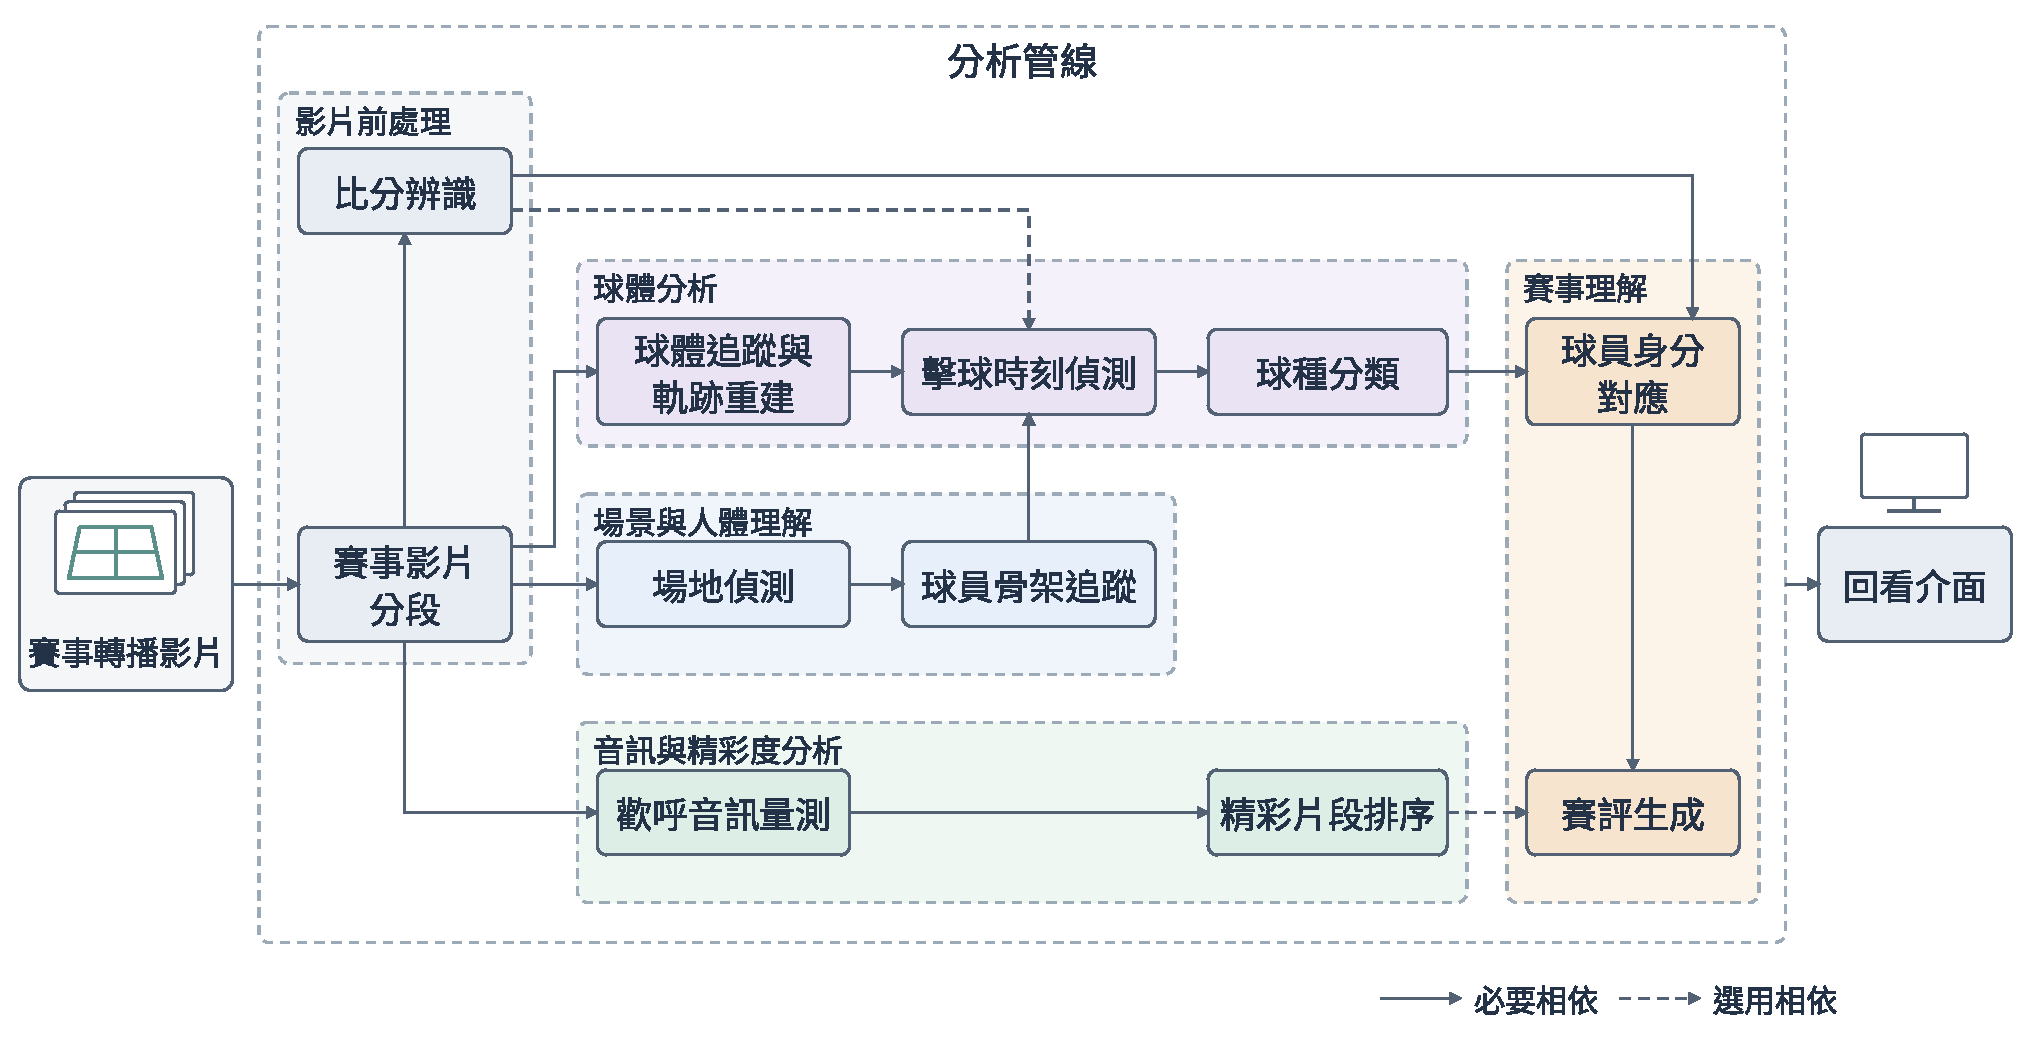
\includegraphics[scale=\flowscale]{system-architecture.pdf}
  \caption{系統架構}
  \label{fig:system-architecture}
\end{figure}

\subsection{管線約定}
\label{sec:pipeline-conventions}

以下四個約定讓各階段能各自開發、單獨執行與重跑。

\begin{enumerate}
  \item \textbf{單一產物、統一格式。}每個階段只寫一個 JSON 產物，外層固定是一個物件、內含一組記錄陣列，記錄欄位由程式中的資料類別統一定義。因為形狀一致，讀寫共用同一組函式，新增階段只需定義資料類別。
  \item \textbf{以完整比賽時間對齊。}所有產物都以原始影片的時間為準，視覺結果記錄絕對影格編號，音訊窗口記錄在整場比賽中的起訖秒數，片段層級的結果則以片段在 \texttt{segments.json} 中的索引對應。
  \item \textbf{產物與快取分離。}每場比賽的 \texttt{cache/} 放昂貴但可重建的中間結果（降解析度影片、TrackNet 熱圖、人體偵測結果、逐幀球種機率）。快取以內容命名並以片段為單位存放，因此中斷可續跑，重新分段時也只有內容改變的片段需要重算。
  \item \textbf{依內容判斷是否重跑。}使用者可只選取部分階段，執行器依相依關係排序後逐一執行，已完成的階段預設跳過。透過比對上游產物的內容雜湊判斷是否跳過。任一階段失敗即停止整條管線。
\end{enumerate}

\begin{table}[H]
  \centering
  \small
  \caption{管線各階段的相依與產物}
  \label{tab:stages}
  \begin{tabularx}{\linewidth}{|>{\raggedright\arraybackslash}p{6.2em}|>{\hsize=.85\hsize}L|>{\ttfamily\footnotesize}l|>{\hsize=1.15\hsize}L|}
    \hline
    階段 & 相依階段 & \normalfont 產物 & 每筆記錄的內容 \\ \hline
    賽事影片分段 & — & segments.json & 一個主機位比賽片段的起訖影格 \\ \hline
    比分辨識 & 分段 & scores.json & 一個片段的比分、發球方與局數；片段內含多個回合時，另記各回合比分與切點 \\ \hline
    場地偵測 & 分段 & court.json & 球場四個外角，以及球場平面與影像之間的單應矩陣 \\ \hline
    球體追蹤與軌跡重建 & 分段 & shuttle.json & 一幀中羽球的座標與可見性，兩種軌跡各一份 \\ \hline
    球員骨架追蹤 & 分段、場地偵測 & pose.json & 一幀中兩名球員的 17 個關節點與人體框 \\ \hline
    擊球時刻偵測 & 球體追蹤、骨架追蹤；選用：比分辨識 & events.json & 一次擊球的影格編號 \\ \hline
    球種分類 & 擊球時刻偵測、骨架追蹤、球體追蹤、場地偵測 & strokes.json & 一次擊球的球種（8 類）、擊球者（畫面上方或下方）與信心 \\ \hline
    歡呼音訊量測 & 分段 & audio\_signals.json & 一個片段的歡呼信心與強度，以及逐窗口的歡呼分數 \\ \hline
    精彩片段排序 & 歡呼音訊量測 & highlights.json & 一個片段的精彩度分數 \\ \hline
    球員身分對應 & 球種分類、比分辨識；選用：骨架追蹤 & identity.json & 兩次換邊之間，上下方球員各對應計分板上的哪位選手，以及判定依據 \\ \hline
    賽評生成 & 分段、擊球時刻偵測、球種分類、比分辨識、身分對應；選用：精彩片段排序、骨架追蹤、場地偵測、球體追蹤 & commentary.json & 一個片段的回合賽評與逐拍賽評 \\ \hline
  \end{tabularx}
\end{table}

\section{影片前處理}
\label{sec:preprocessing}

\subsection{賽事影片分段}
\label{sec:match-segmentation}

\subsubsection{概述}

\textbf{問題與目標：}一支羽球轉播影片中，適合進行球員、羽球軌跡分析的畫面，主要來自固定俯拍的機位。若系統直接分析整部影片，非固定機位比賽畫面會產生大量錯誤資料，也浪費運算資源。本模組從轉播影片中找出固定機位比賽畫面，作為後續模組的輸入。

\textbf{設計重點：}本模組不需額外訓練模型、標註資料，也不需針對每支影片逐片人工調整參數，依據影片的統計結構自適應於不同影片。核心設計是把「固定機位比賽畫面主要只有球員移動」這個先驗，轉化為影格差異訊號。固定機位比賽片段的相鄰影格差異小、運鏡與鏡頭切換差異大、靜止的計分板差異極小，因此只用一個廉價的差異指標（MAD）就能把固定機位比賽片段與其他畫面在數值上分開。另一個核心設計是利用「同一機位在不同片段間具有高度相似性」，排除計分板、重播及其他靜止畫面。在 9 場未參與開發的比賽上，片段偵測 F1 達 98.66\%（見\secref{sec:exp-segmentation}）。

\textbf{處理流程總覽：}如\figref{fig:match-segmentation-flow}。

\begin{figure}[H]
  \centering
  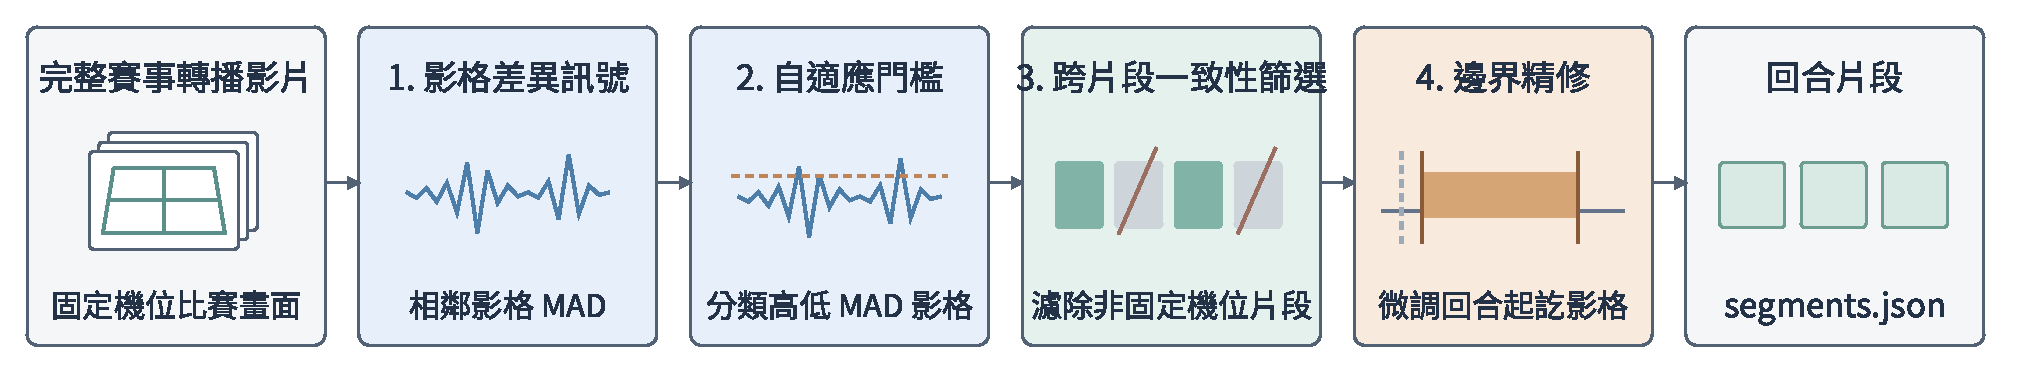
\includegraphics[scale=\flowscale]{match-segmentation.pdf}
  \caption{賽事影片分段處理流程}
  \label{fig:match-segmentation-flow}
\end{figure}

\subsubsection{影格差異訊號}

固定機位比賽片段畫面中只有兩名球員與球在動，兩影格間的差異小。其餘片段則落在兩個極端，鏡頭移動與切換使差異極大，靜止的計分板與定格畫面則差異極小。本模組以影格與影格之間的差異作為核心訊號。差異以 MAD（平均絕對差，Mean Absolute Difference）衡量：
\begin{equation}
  \mathrm{MAD} = \frac{1}{MN}\sum_{x=1}^{M}\sum_{y=1}^{N} \left| I_1(x,y) - I_2(x,y) \right|
  \label{eq:mad}
\end{equation}
其中 $M$、$N$ 為影像寬高，$I(x,y)$ 為座標 $(x,y)$ 的灰階值。選用 MAD 的理由是成本低廉、對離群值不敏感、且動態範圍足夠。計算前先將影片縮放至 480p 以減少計算量。MAD 不隨解析度改變，相對高低仍然成立。

取樣採每隔三個影格一次，並與前一個取樣影格計算 MAD。間隔取樣一方面縮短處理時間，一方面避免特寫片段和固定機位比賽片段混淆。特寫中球員動作緩慢、背景固定，MAD 偏低且接近固定機位比賽片段，間隔取樣把緩慢位移放大、拉高其 MAD。固定機位比賽片段中球員佔比小、動作劇烈，間隔取樣影響有限。兩類片段因此在 MAD 上分開。

\begin{figure}[H]
  \centering
  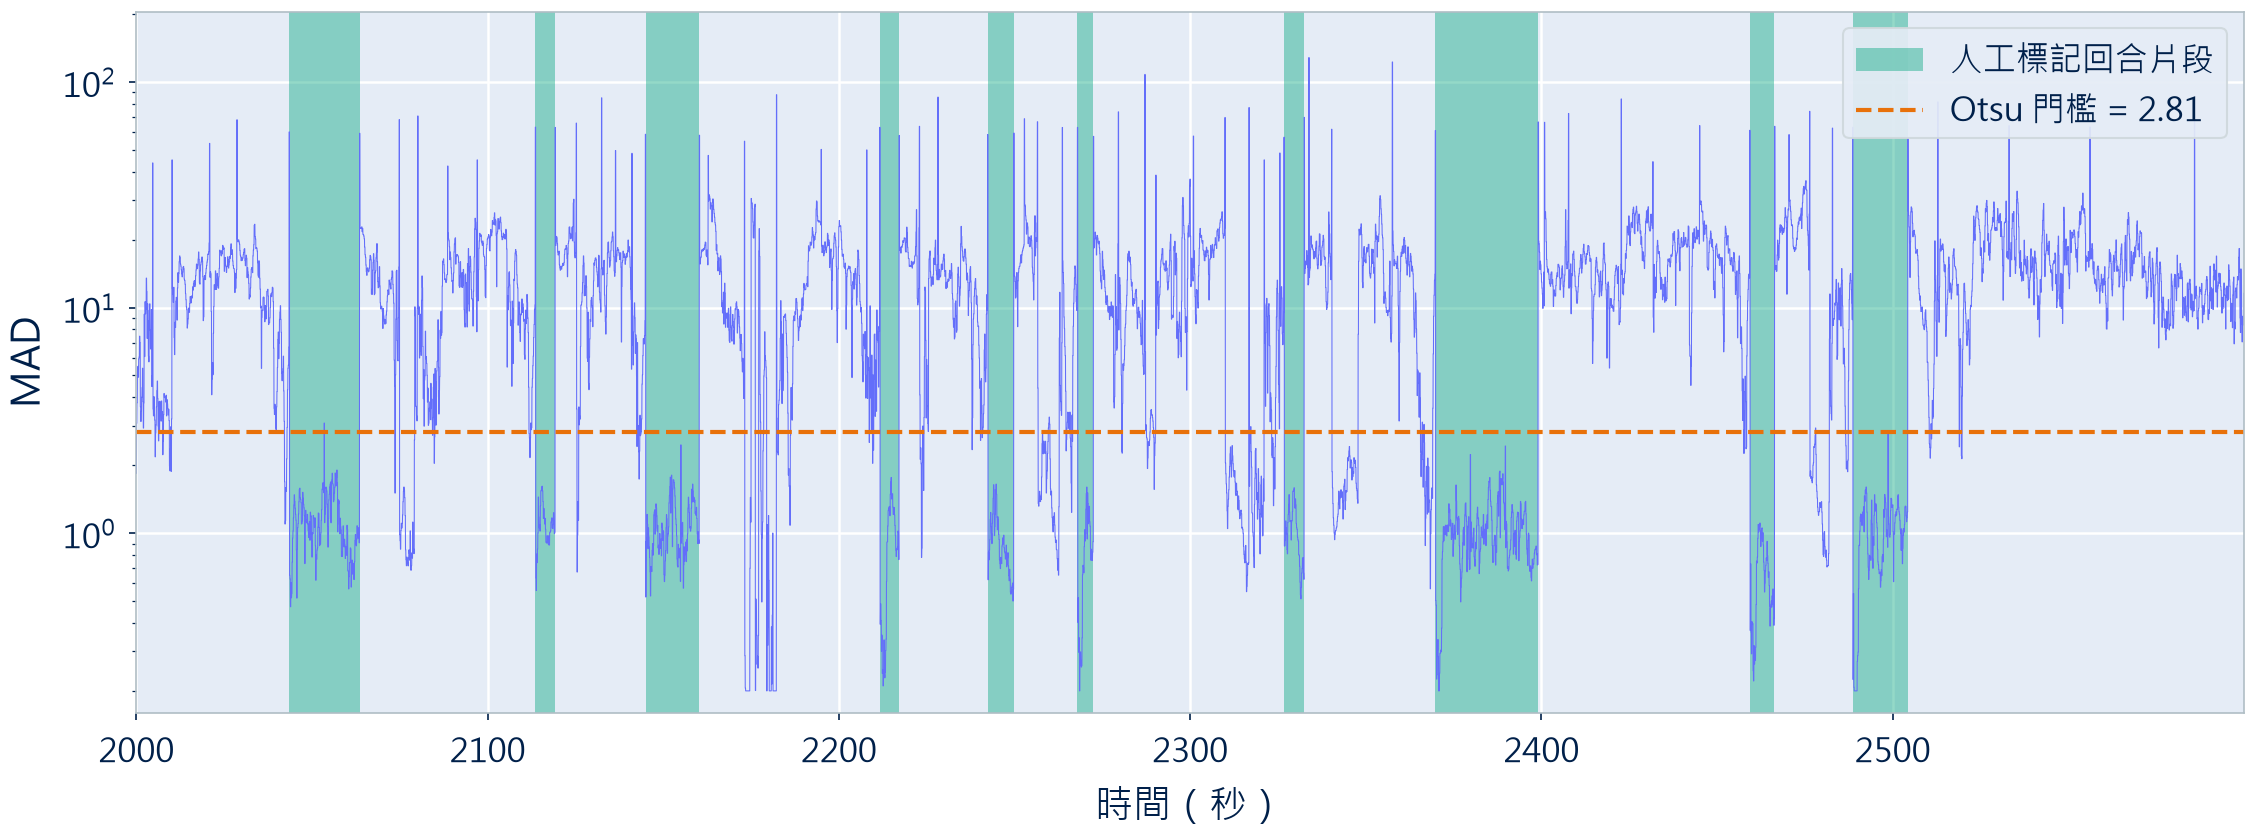
\includegraphics[width=\linewidth]{match_segmentation/mad_timeline.png}
  \caption{部分片段 MAD}
  \label{fig:mad-timeline}
\end{figure}

\figref{fig:mad-timeline}中綠色區塊為手動標記的固定機位比賽片段，虛線為系統算出的門檻，可見綠色區塊的 MAD 通常低於門檻。

\subsubsection{自適應門檻}

本階段統計全片的 MAD 分佈，設定一個門檻把影格分成低 MAD（固定機位比賽畫面、靜止畫面）與高 MAD（運鏡、鏡頭切換）。不同影片的分佈不同，門檻須隨影片自動調整。

分析前先對 MAD 取以 10 為底的對數。鏡頭切換到完全不同畫面時每個像素都不一樣，會產生極大 MAD，使分佈右側出現長尾。取對數可壓縮長尾，使高低兩側尺度相當。實作取 $\log_{10}(\max(\mathrm{MAD}, 1))$，因為 MAD 可能為 0，需要地板值 1。

\begin{figure}[H]
  \centering
  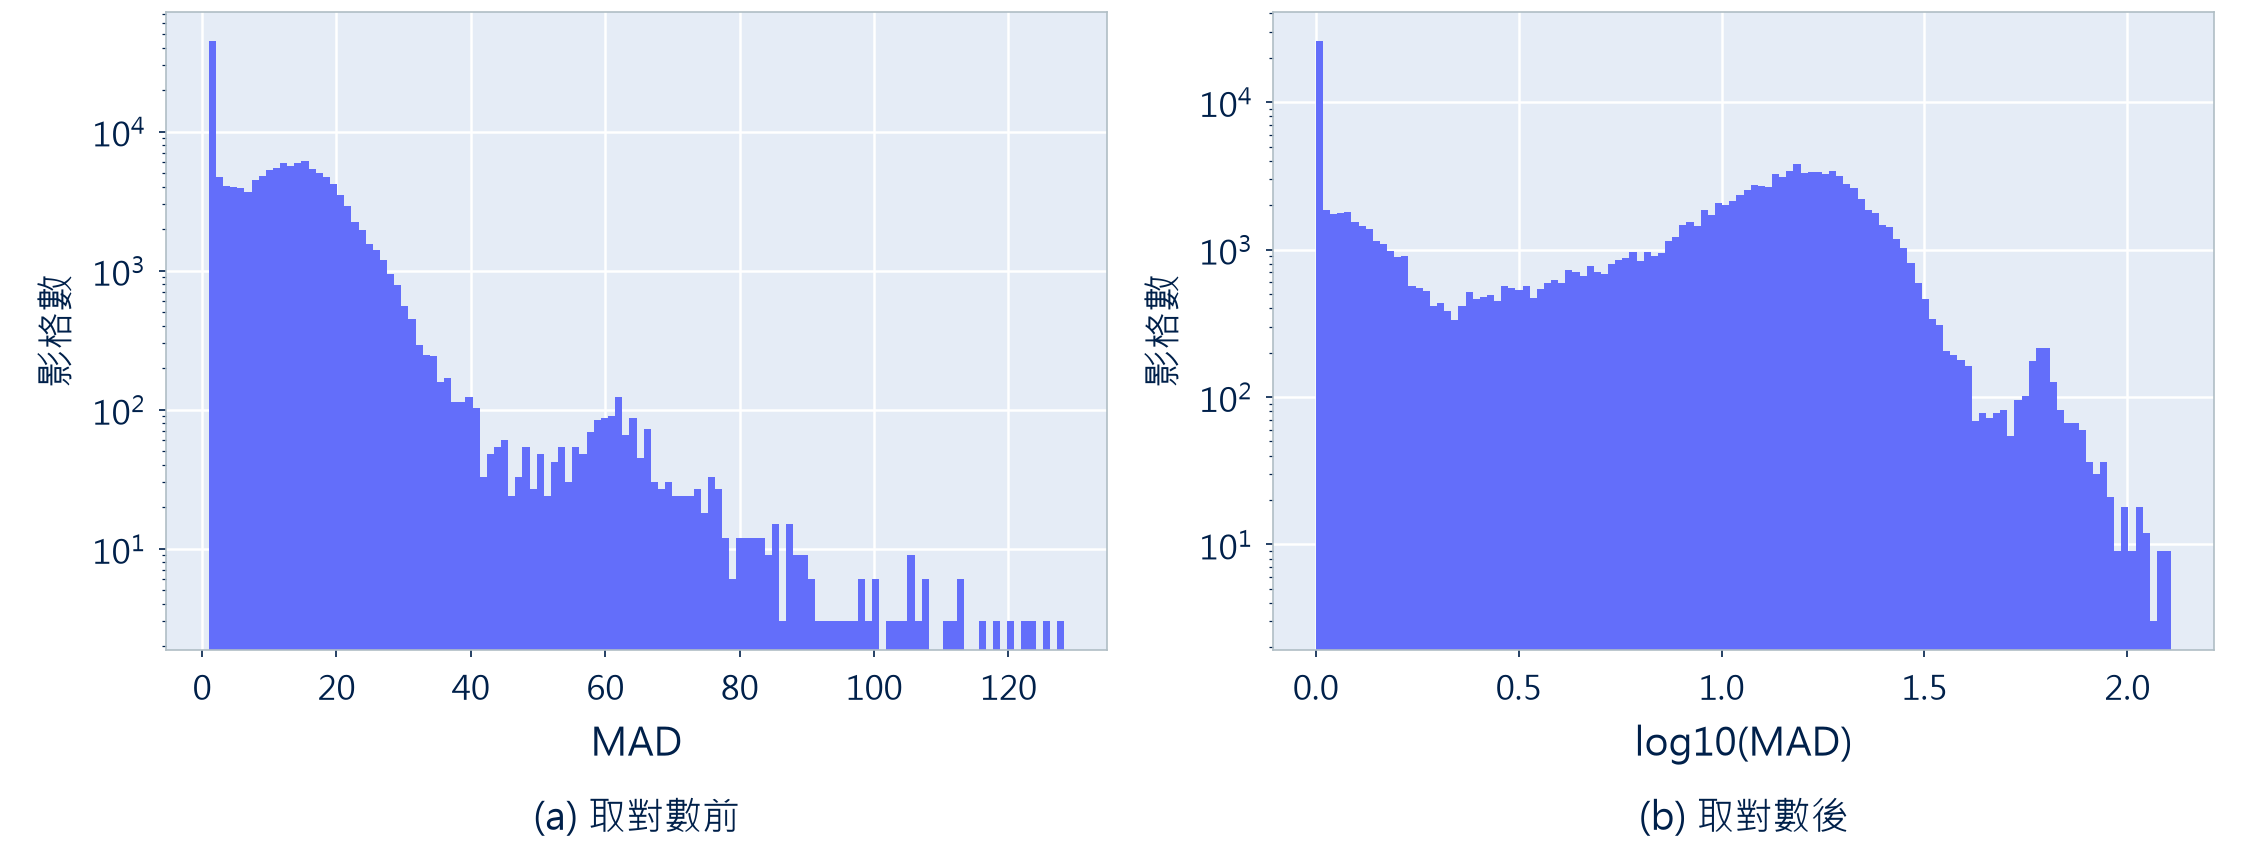
\includegraphics[width=\linewidth]{match_segmentation/log_transform.png}
  \caption{取對數}
  \label{fig:log-transform}
\end{figure}

\textbf{乾淨片段偵測：}若輸入本身無鏡頭切換，重尾程度會遠低於多鏡頭影片，據此判定乾淨固定機位片段，跳過後續步驟直接輸出。

\textbf{門檻方法：}設門檻的問題與影像二值化相似，二值化統計像素亮度並切成兩類，本階段統計影格 MAD 並切成兩類，故沿用二值化的門檻計算方法。本系統採 Otsu 法，它只要求兩類均值不同即可分離，不限制分佈形狀、不需調參，正好適用於本階段低 MAD 側有尖峰、高 MAD 側是不對稱長尾的情形。

\begin{figure}[H]
  \centering
  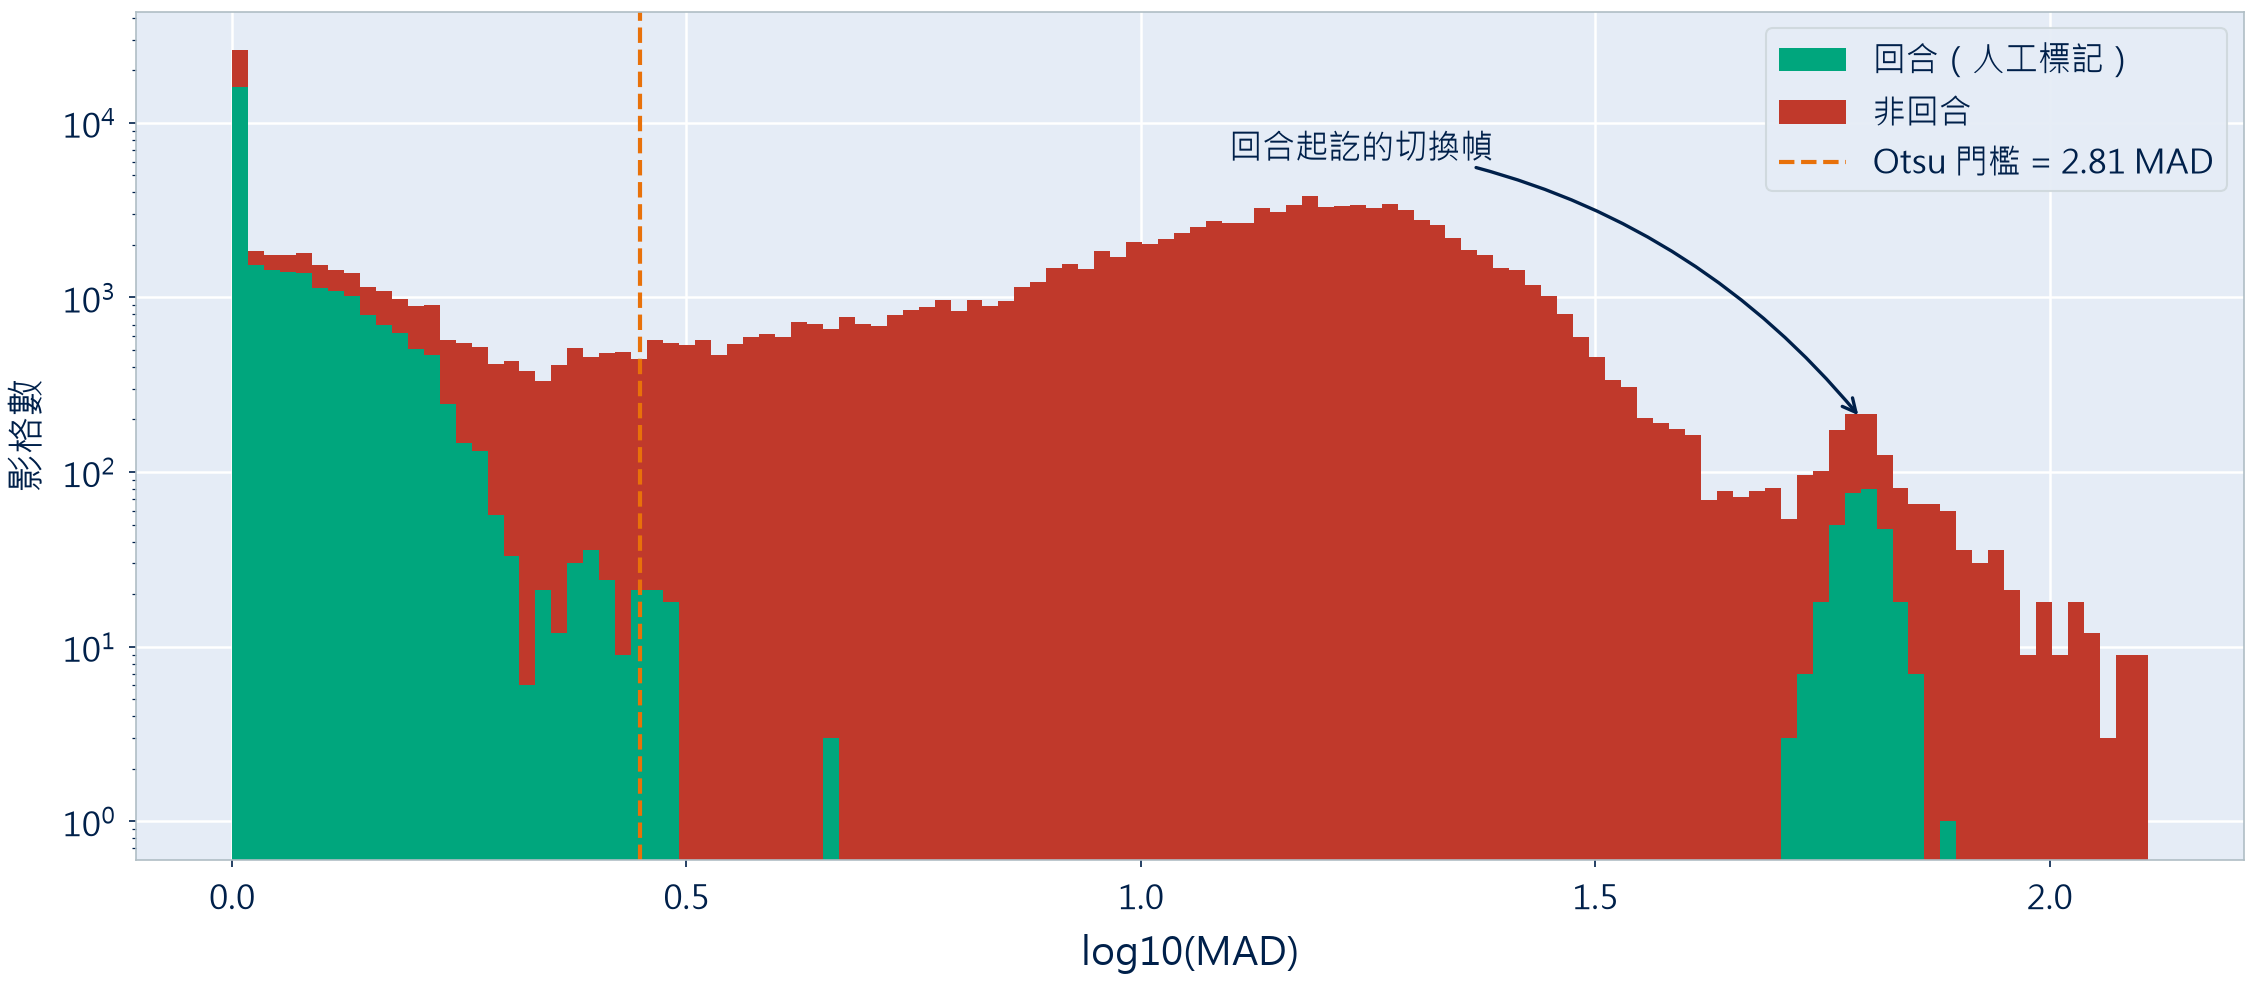
\includegraphics[width=\linewidth]{match_segmentation/rally_split_hist.png}
  \caption{固定機位比賽片段與其他片段的 MAD 分佈}
  \label{fig:rally-split-hist}
\end{figure}

\begin{table}[H]
  \centering
  \caption{$\log_{10}(\mathrm{MAD})$ 的分佈與組成}
  \label{tab:mad-composition}
  \begin{tabular}{|l|r|r|l|}
    \hline
    MAD 區間 & 佔全片比例 & 固定機位比賽比例 & 畫面性質 \\ \hline
    0--0.5 & 6.8\% & 28\% & 近乎靜止 \\ \hline
    0.5--2 & 23\% & 75\% & 固定機位比賽畫面 \\ \hline
    2--2.75 & 2.3\% & 5\% & 谷底，門檻落點 \\ \hline
    2.75--30 & 65\% & 約 0\% & 重播、運鏡 \\ \hline
    30 以上 & 2.8\% & 7\% & 快速轉場 \\ \hline
  \end{tabular}
\end{table}

\textbf{三類切分：}直接做兩類 Otsu 會產生系統性偏差，高 MAD 側佔全片 68\% 且橫跨 2.75 至 128，類內變異遠大於低 MAD 側，會把切點從谷底推進高 MAD 團內部，讓大量非固定機位比賽影格進入下一步。改用三類切分，上切點（10.80）吸收長尾壓力，下切點（2.81）回到谷底，取下切點為門檻（\figref{fig:otsu-3class}）。三類 Otsu 的效果等價於先移除長尾再做兩類 Otsu。

\begin{figure}[H]
  \centering
  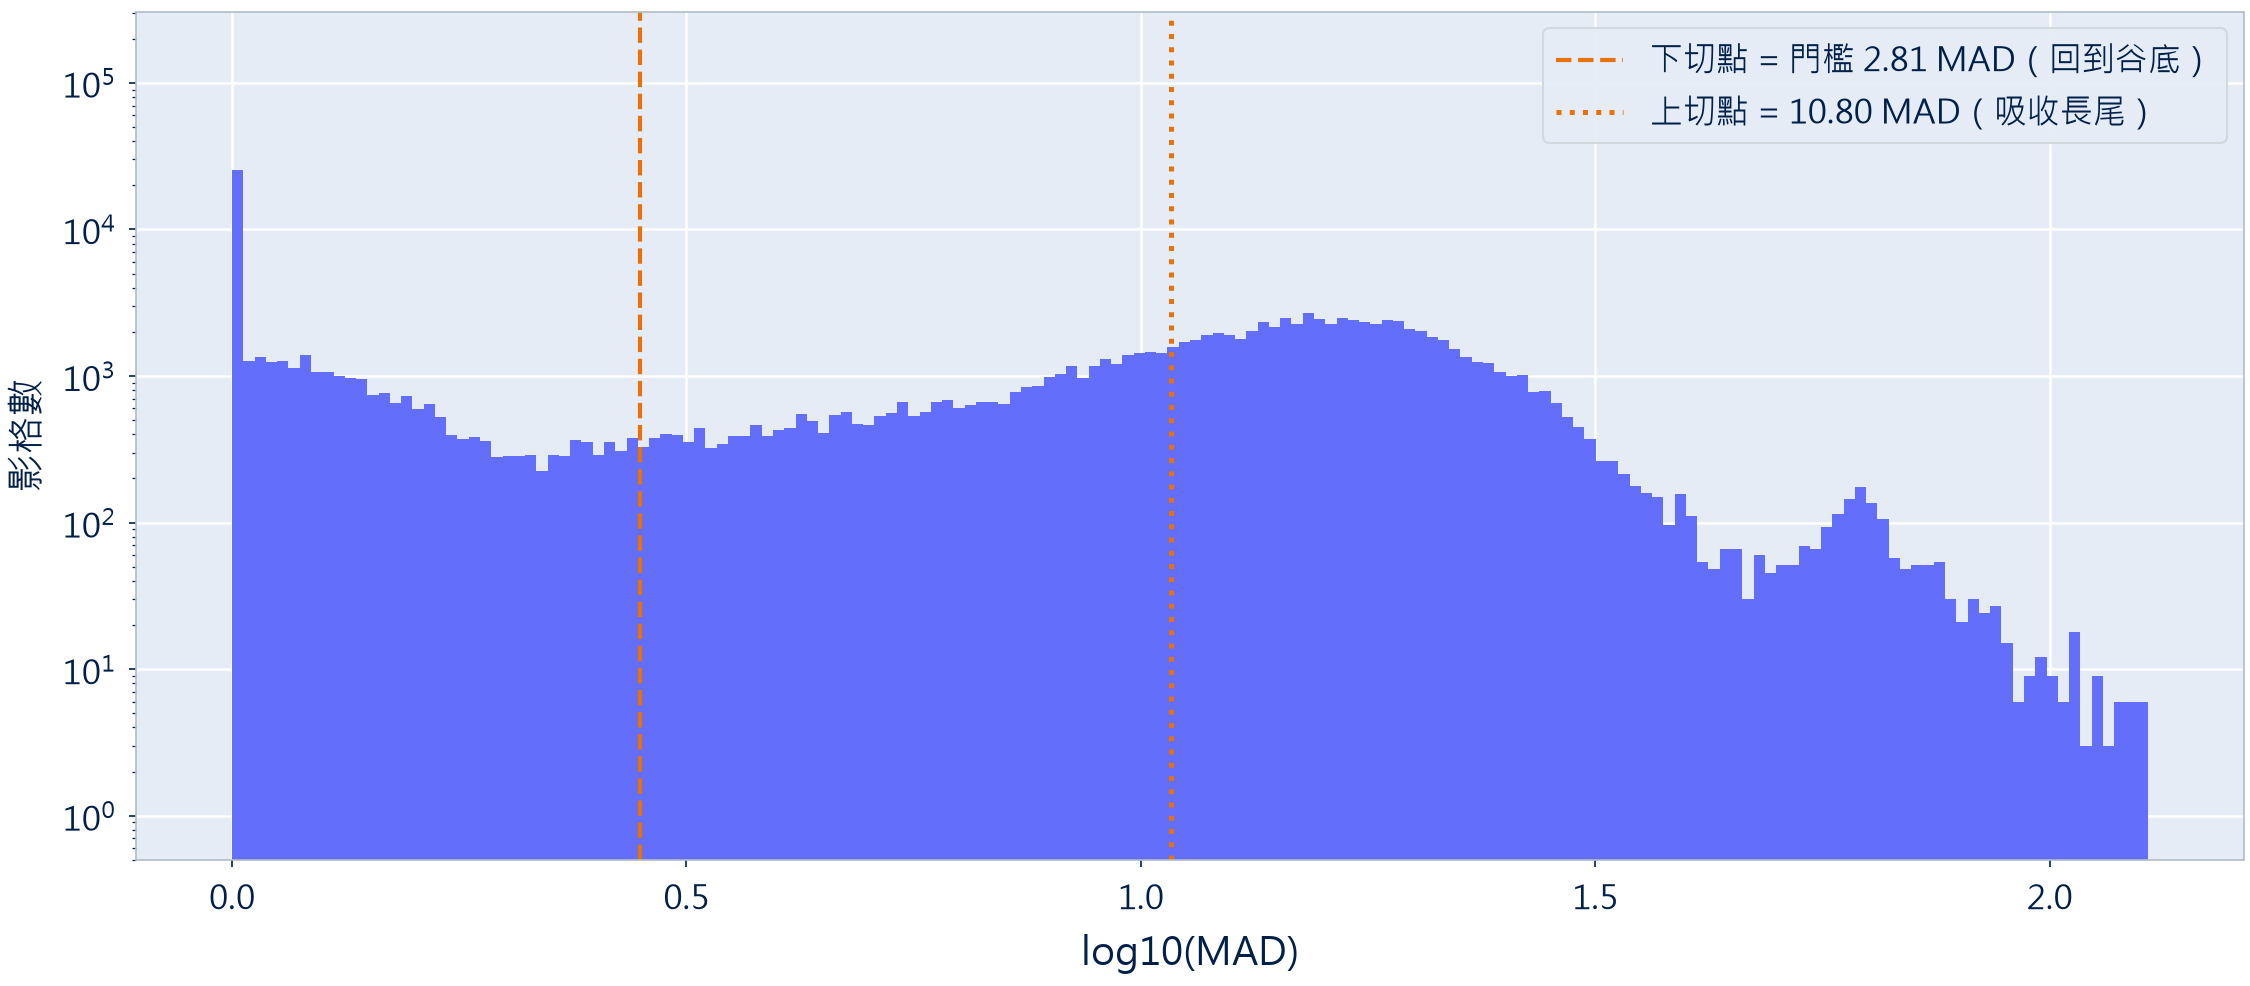
\includegraphics[width=\linewidth]{match_segmentation/otsu_3class.png}
  \caption{三類 Otsu 的兩個切點}
  \label{fig:otsu-3class}
\end{figure}

\subsubsection{跨片段一致性篩選}

將連續低 MAD 影格串接成片段，此時保留下來的片段中仍混有計分板、定格等靜止片段。關鍵觀察是，此時剩餘的固定機位比賽片段數量多，且全部來自同一個固定機位、彼此在畫面上高度相似。其他片段則各自不同，與任何片段都不像。因此可以透過片段之間相互比較，判斷一個片段是否屬於佔多數的固定機位比賽片段。

設共有 $N$ 個片段，片段 $i$ 取其中央兩張影格，各自縮放至 $128\times72$ 並展開為特徵向量 $v_i^{(1)}, v_i^{(2)}$。兩片段的差異 $d(i,j)$ 取四組跨影格 MAD 的平均，跨片段平均差異 $\bar{d}(i)$ 則是片段 $i$ 對其餘 $N-1$ 段的平均：
\begin{equation}
  d(i,j) = \frac{1}{4}\sum_{a=1}^{2}\sum_{b=1}^{2} \mathrm{MAD}\!\left(v_i^{(a)},\, v_j^{(b)}\right),
  \qquad
  \bar{d}(i) = \frac{1}{N-1} \sum_{j \neq i} d(i,\, j)
  \label{eq:cross-mad}
\end{equation}

\begin{figure}[H]
  \centering
  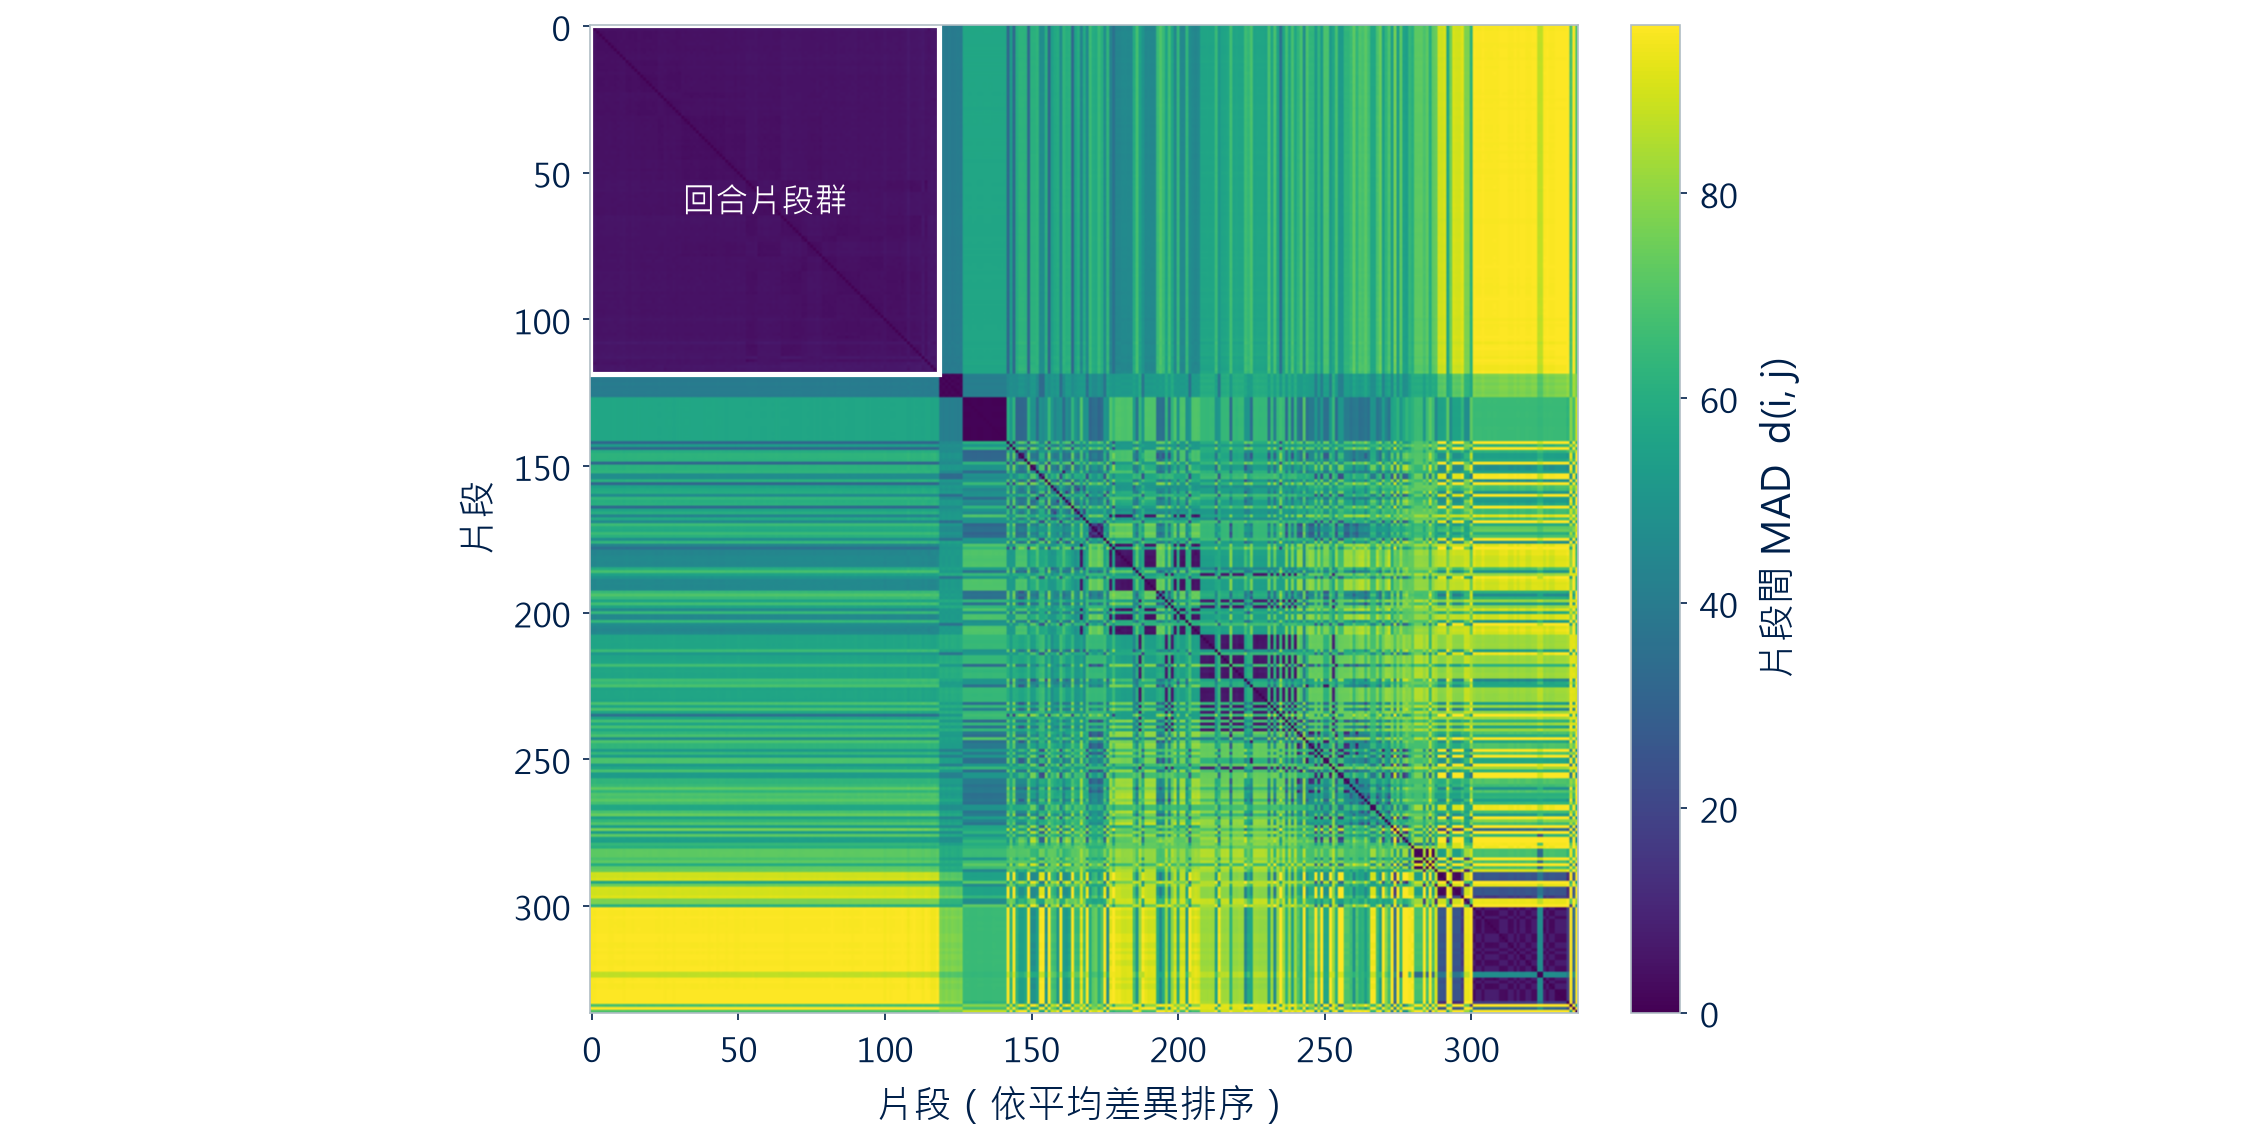
\includegraphics[width=\linewidth]{match_segmentation/cross_matrix.png}
  \caption{跨片段兩兩 MAD 矩陣（依平均差異排序）}
  \label{fig:cross-matrix}
\end{figure}

因為所有固定機位比賽片段高度相似，它的 $\bar{d}(i)$ 幾乎只由少數幾個非固定機位比賽片段貢獻，數值因而偏低。又因固定機位比賽片段彼此相像，算出的 $\bar{d}(i)$ 也幾乎相等，於是它們在直方圖最左側聚成一個緊密的群。其他片段畫面各異，$\bar{d}(i)$ 偏高且分散。\figref{fig:cross-matrix}將片段依 $\bar{d}(i)$ 排序，左上角的紫色密集區即這群固定機位比賽片段。

實測固定機位比賽片段間 $\bar{d}(i)$ 的極差在 5\% 以內，最小的非固定機位比賽片段比全體最小值大 13\%，門檻取全體最小值的 1.07 倍（\figref{fig:cross-avg}）。此門檻成立的前提是固定機位比賽片段屬於最緊密的群，若影片含大量彼此相似的畫面，會形成新的低 $\bar{d}(i)$ 群使門檻失效。

\begin{figure}[H]
  \centering
  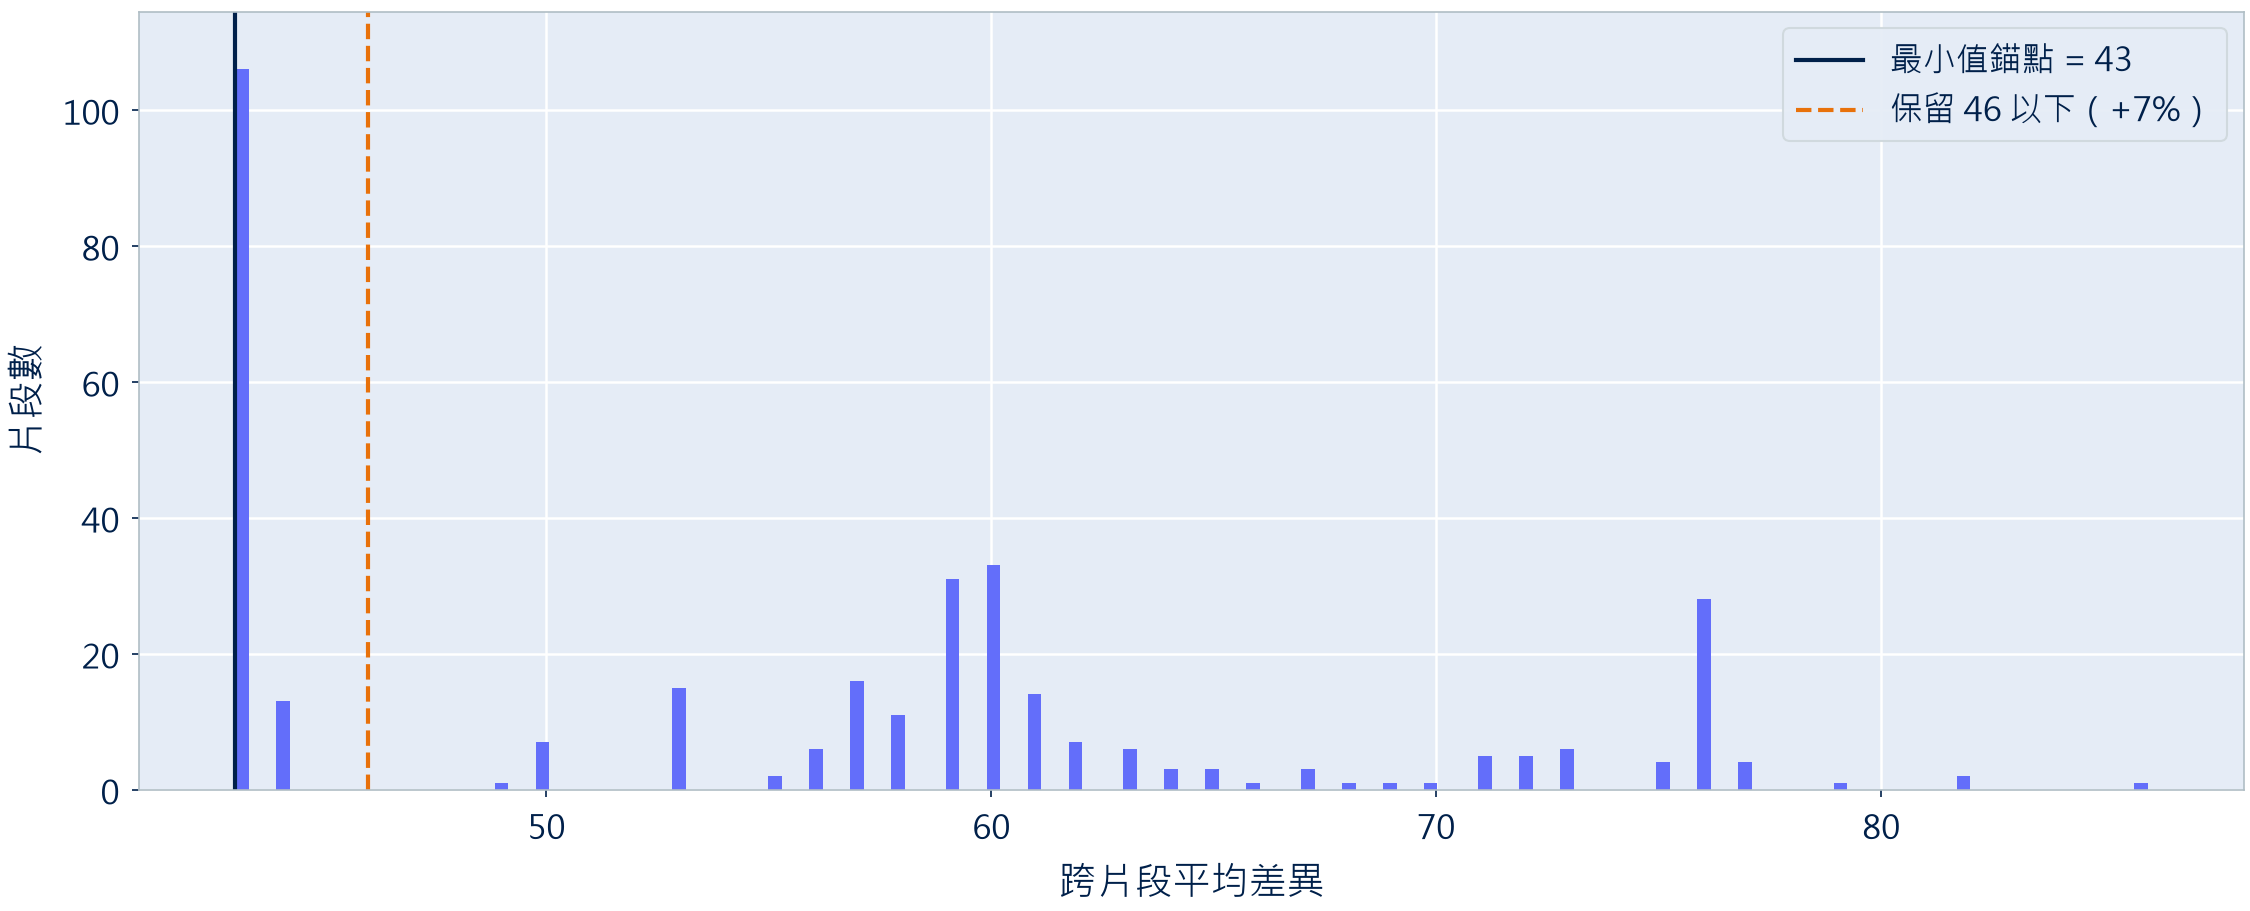
\includegraphics[width=\linewidth]{match_segmentation/cross_avg.png}
  \caption{跨片段平均差異的分佈與門檻}
  \label{fig:cross-avg}
\end{figure}

通過篩選的片段中偶爾仍殘留鷹眼判定、官方重播等電腦合成畫面，其構圖與固定機位比賽畫面接近。因此對剩餘片段再算一次跨片段平均差異，採較嚴格的門檻，捨棄超過中位數三倍者。

\subsubsection{邊界精修}

此階段把被少數高 MAD 影格（分數卡片動畫）切碎的片段接回。同時第一階段的跳幀取樣使邊界存在系統性偏差，需還原到影格層級。

\textbf{做兩次片段連接：}第一次只看距離，間距小於 5 張影格的相鄰片段直接接合。第二次針對 12 張影格以內的間隙逐影格重新掃描，僅當間隙內最大相鄰 MAD 低於 25（即不存在尖峰）時才接合。

\textbf{做邊界對齊：}在每個邊界附近逐影格計算相鄰 MAD，尋找同時滿足絕對值門檻與區域中位數倍率的尖峰，此尖峰對應剪接點，起點設為切入尖峰所在的影格，終點設為切出尖峰的前一張影格。

\begin{figure}[H]
  \centering
  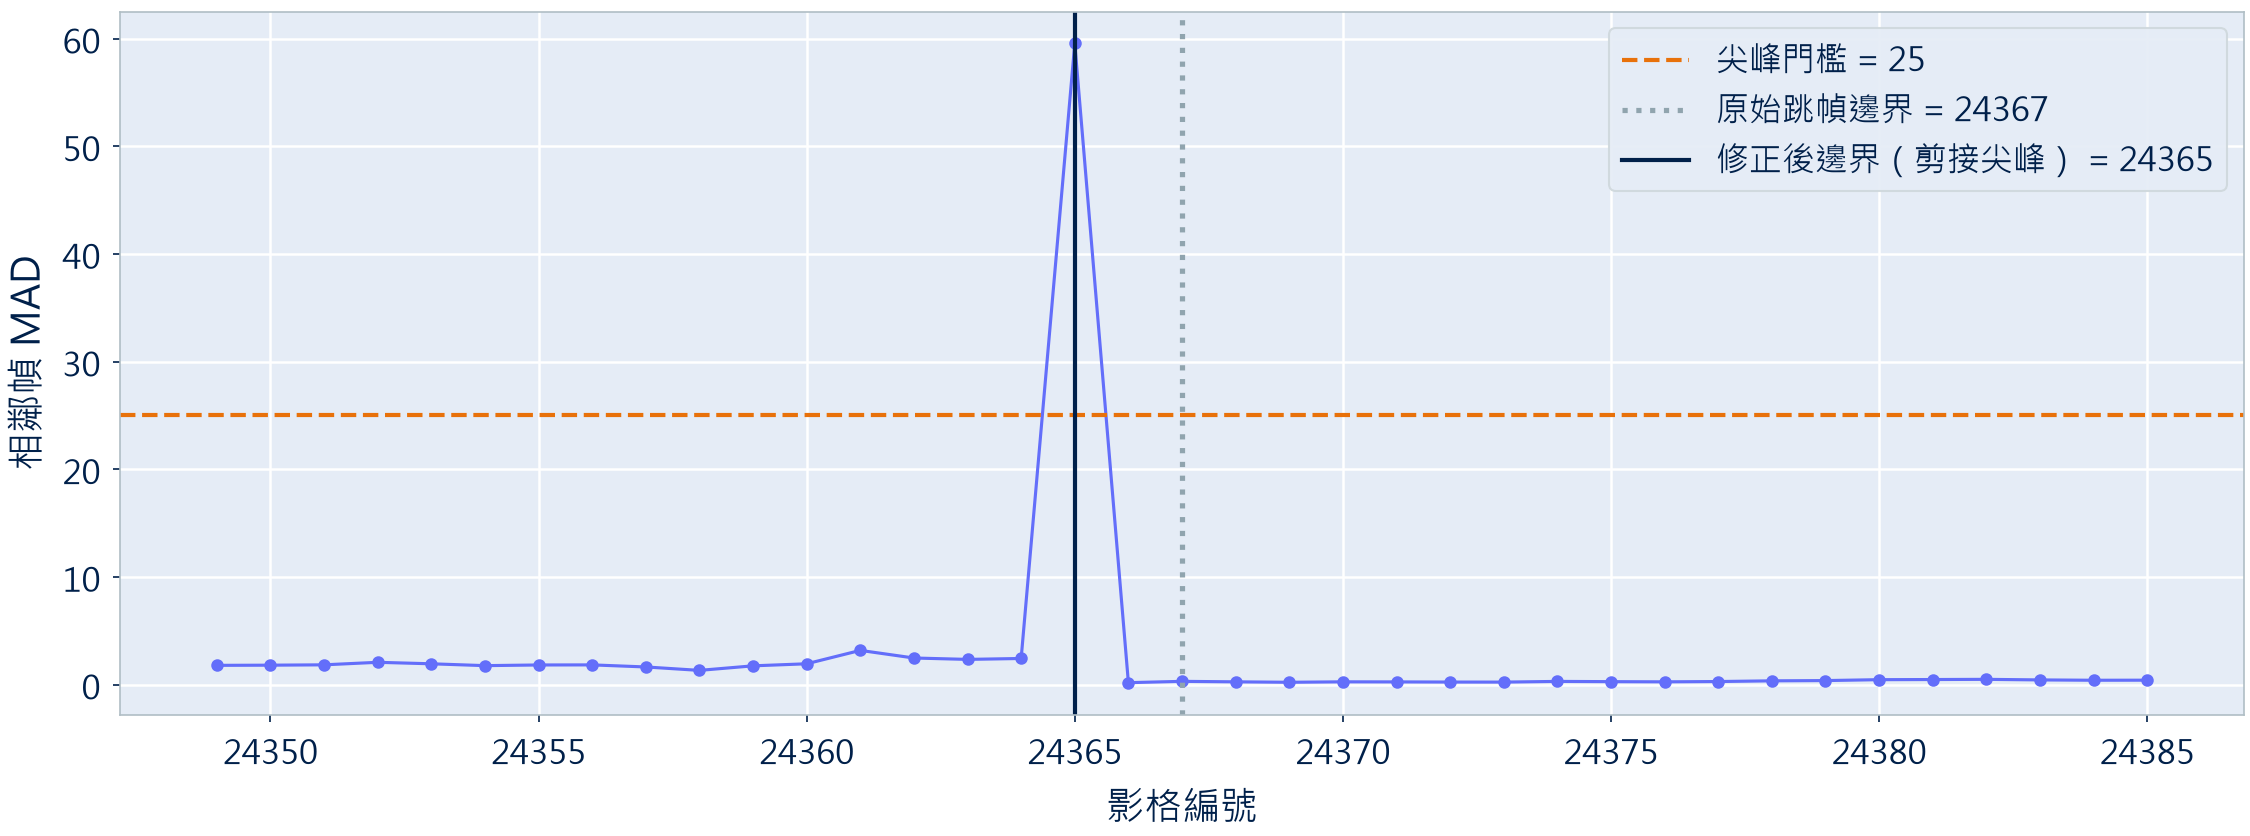
\includegraphics[width=\linewidth]{match_segmentation/cut_spike.png}
  \caption{邊界尖峰偵測與修正}
  \label{fig:cut-spike}
\end{figure}

\figref{fig:cut-spike}中灰色點線為原始跳幀取樣邊界，深藍實線為修正後的邊界，橘色虛線為尖峰門檻。

\subsection{比分辨識}
\label{sec:score-recognition}

\subsubsection{概述}

\textbf{問題與目標：}賽事影片分段模組切出的片段中，同一回合可能因中間插入重播、特寫而被切成數段，一個片段也可能因為沒有鏡頭切換而包含多個回合。本模組為每個片段讀出畫面上的計分板比分，判斷片段所屬的回合，該比分同時供下游精彩片段分析使用。

\textbf{設計重點：}讀計分板天生受三個困難制約：泛化性（各賽事的計分板設計、位置不固定，且須避開干擾文字）、可讀性（計分板小又模糊）、多局制（三局制計分板易讀錯局）。本模組不需訓練模型或逐賽事調參，以「把難題拆成模型擅長的小任務、再用程式補上模型不擅長的部分」為核心，有三點做法：

\begin{enumerate}
  \item \textbf{使用視覺語言模型（VLM）：}目前使用傳統 OCR 的開源專案都需要手動標記計分板的位置。VLM 直接理解畫面結構，依視覺上下文自行分辨比分。不用為每種計分板寫過濾規則或手動標記，提升跨賽事的泛化能力。
  \item \textbf{多幀合成：}利用逐像素合成，強化計分板、糊化背景和球員。在 overlay 只出現於三成影格時仍能完整還原。
  \item \textbf{提示詞設計：}轉錄取代挑選，令模型由左到右完整抄寫計分板上所有數字（模型擅長），把當前局比分的挑選（模型易錯）移到程式端，讓較便宜的模型也能快速、正確的完成任務。
\end{enumerate}

\textbf{處理流程總覽：}如\figref{fig:score-recognition-flow}。

\begin{figure}[H]
  \centering
  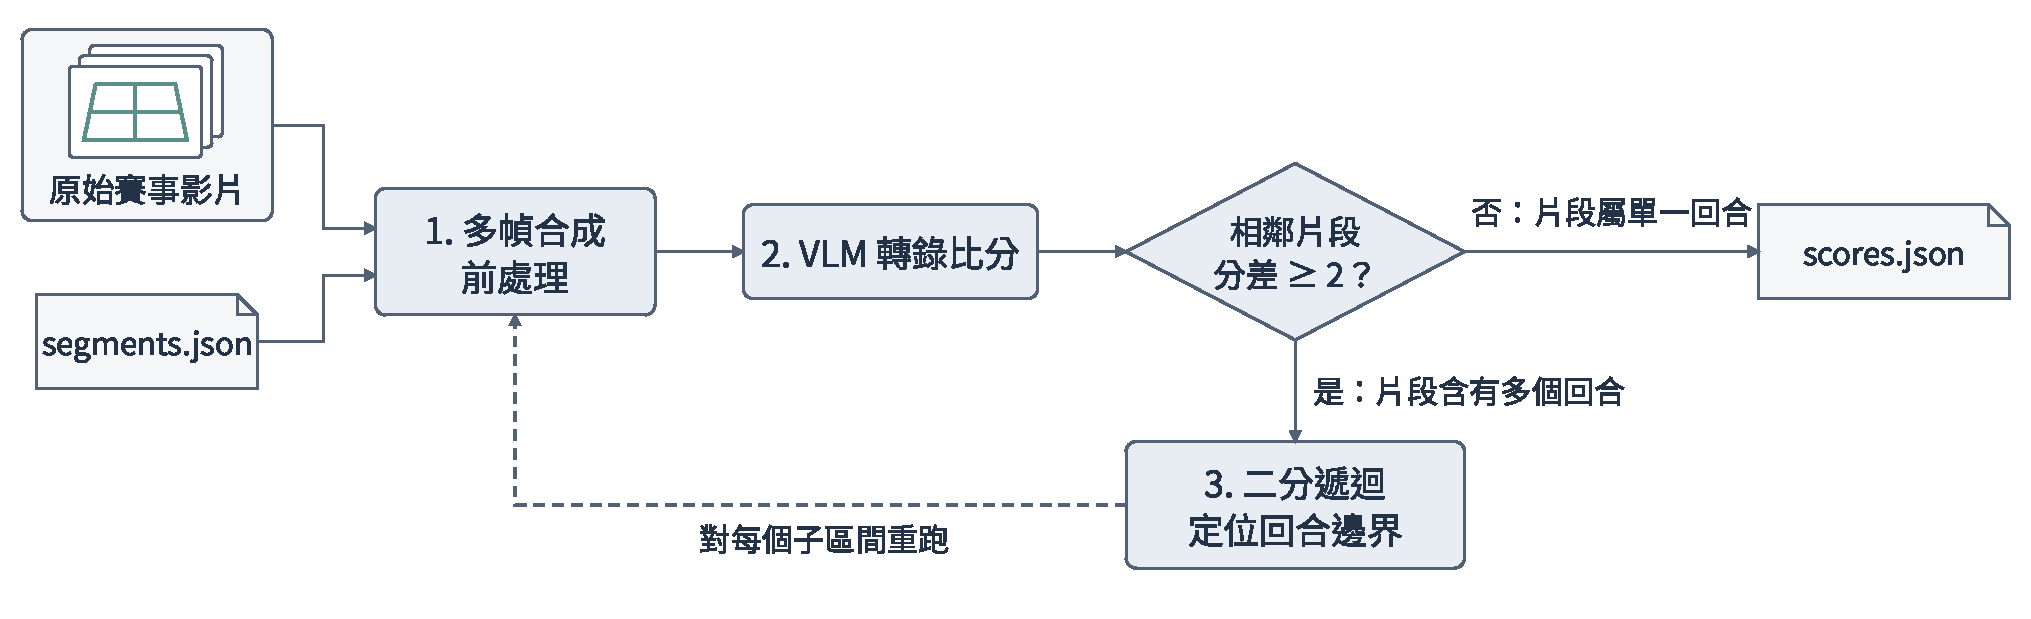
\includegraphics[scale=\flowscale]{score-recognition.pdf}
  \caption{比分辨識處理流程}
  \label{fig:score-recognition-flow}
\end{figure}

\subsubsection{多幀合成前處理}

本步驟為每個片段產生一張合成圖，讓 VLM 讀一張圖就拿到比分。轉播的計分板 overlay 只在片段的部分影格出現，若逐張送 VLM 去找，每個片段都得呼叫多次。一個片段通常同屬一回合，比分不變、計分板靜態，因此把片段取樣的多張影格逐像素合成，間歇出現的計分板被疊加強化、穩定呈現在合成圖上，一個片段只需一次 API 呼叫。不斷移動的球員與觀眾被平均糊化，順帶為 VLM 濾去干擾。

合成採 \texttt{dominant\_cluster}（主群集平均）：對每個像素的亮度值分箱，只平均落入最多值的那一箱。overlay 出現時亮度幾乎固定，會全擠進同一箱。背景每幀不同而分散各箱。因此最密集的一簇即為計分板（\figref{fig:overlay-recovery}）。這個方法不預設目標信號在時間上佔多數，即使轉播 overlay 只間歇出現仍能保留。

\begin{figure}[H]
  \centering
  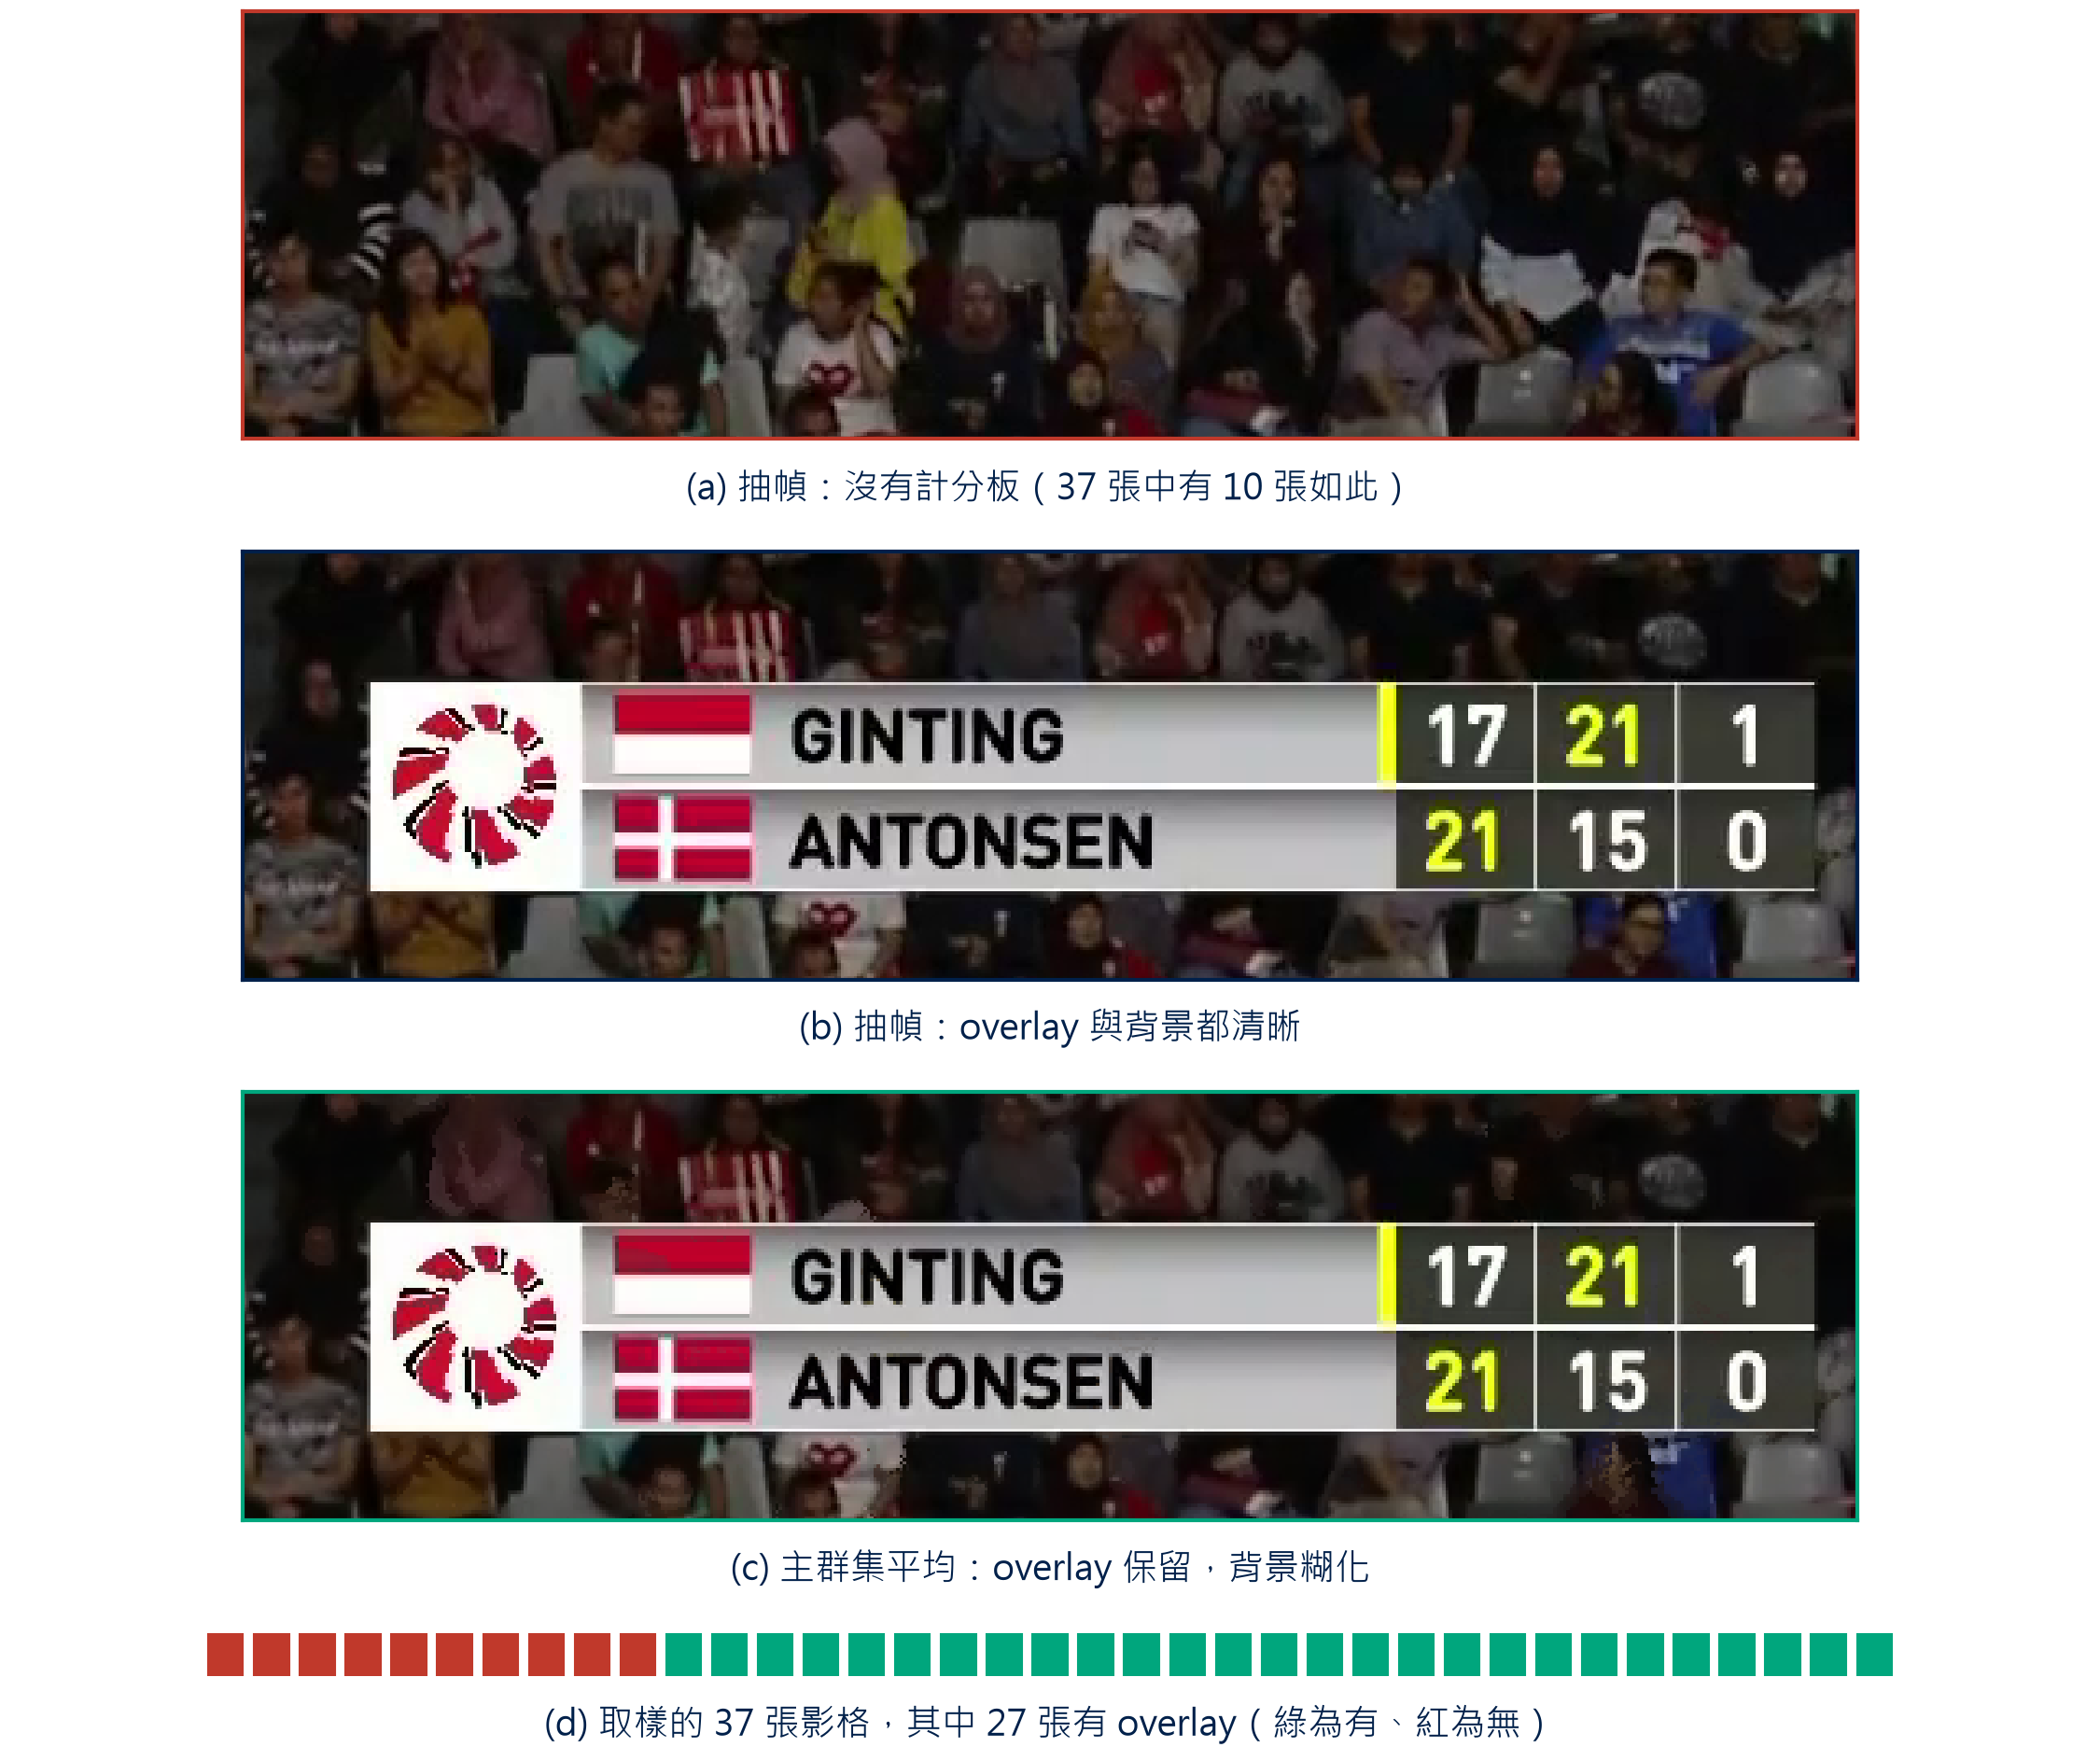
\includegraphics[width=\linewidth]{score_recognition/overlay_recovery.png}
  \caption{overlay 只出現在部分影格時，主群集平均的還原結果}
  \label{fig:overlay-recovery}
\end{figure}

\subsubsection{VLM 轉錄比分}

本步驟從合成圖讀出雙方當前比分。多局制計分板每隊並列多局數字，要模型直接判斷「哪個是當前局」容易錯，完整抄寫數字對模型來說不需要推理，比較簡單。因此只要求模型逐隊由左到右抄下所有數字，挑選交給程式，固定取每隊陣列最右一個為當前比分，從根源消除模型讀錯局的可能（\figref{fig:transcription-pick}）。

實作上使用 Gemini 2.5 Flash，將 temperature 設為 0，並且關閉 thinking，減少結果變化的同時避免模型進行不必要的推理，多餘的推理浪費 token、時間又容易出錯。

\begin{figure}[H]
  \centering
  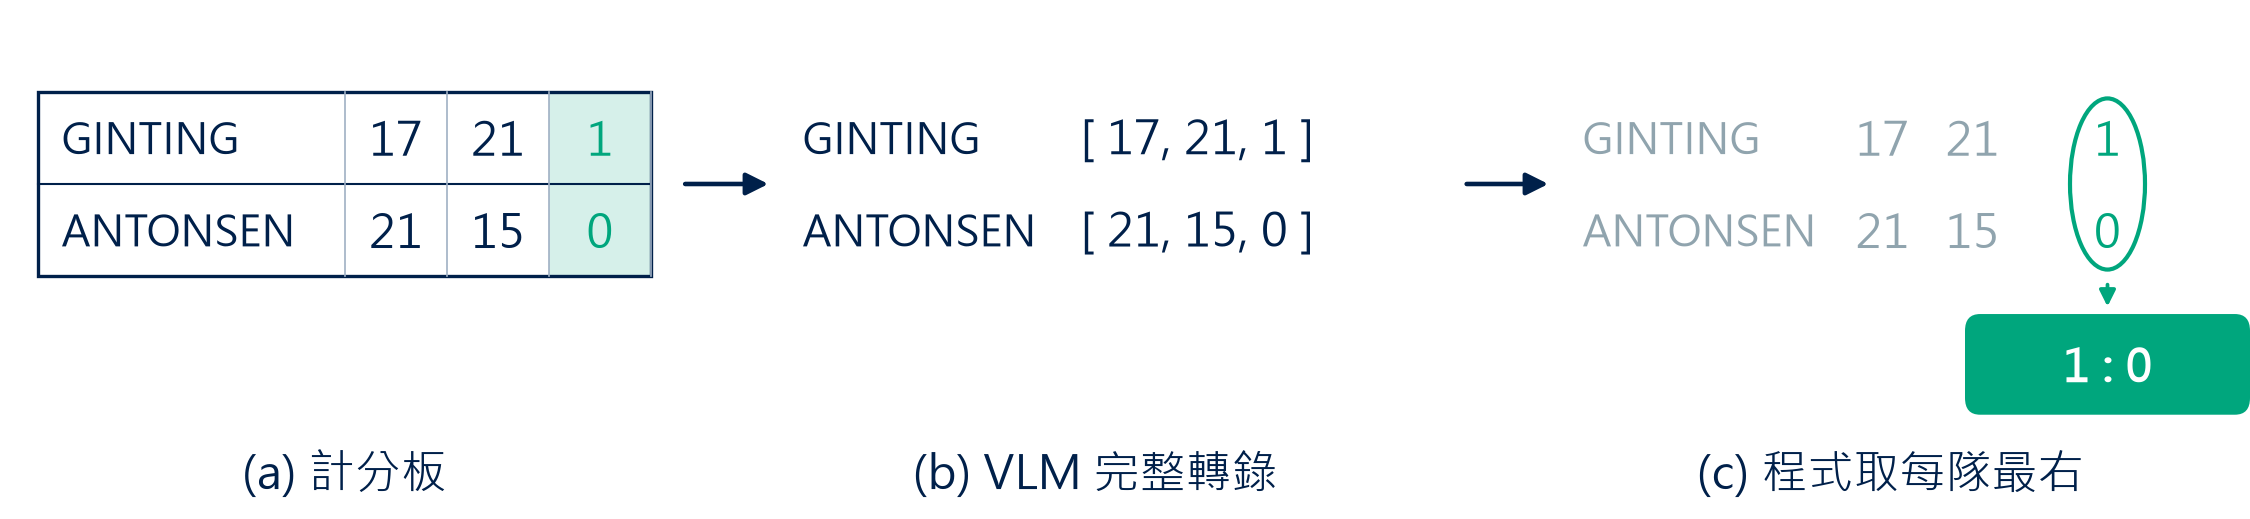
\includegraphics[width=\linewidth]{score_recognition/transcription_pick.png}
  \caption{轉錄取代挑選，VLM 完整抄寫每隊數字，程式取最右一個為當前比分}
  \label{fig:transcription-pick}
\end{figure}

\subsubsection{還原被合併的回合}

分段以鏡頭切換為訊號，兩回合間若沒有切換就會被併進同一片段，此時計分板在片段中途變動，單張合成只讀得到其中一個回合。本步驟負責找出並拆開這類片段。

判斷靠比分本身，正常一回合雙方總分只加一分，因此若某片段雙方比分總和一次增加兩分以上，就代表中間有回合沒被單獨切出，標記為合併片段。

標記後以二分搜尋定出回合交界，在候選區間中點重新合成、辨識比分，與兩端比較，往比分仍有跳變的一側收斂，逼近比分改變的影格。由於一個片段可能併入不只兩回合，每定出一個切點就對兩側子區間各自遞迴、繼續二分，直到每個子區間都只差一回合。

\section{場景與人體理解}
\label{sec:scene-understanding}

\subsection{場地偵測}
\label{sec:court-detection}

\subsubsection{概述}

\textbf{問題與目標：}後續所有球員與球體分析需要以球場座標來解讀位置與距離。本模組從固定俯拍的轉播畫面中定出球場，建立影像平面與球場平面投影的座標基準，供後續步驟使用。

\textbf{設計重點：}本模組不需訓練模型、不需標註，核心是把球場偵測化約為「在畫面中找四個外角」的問題，球場是平面、尺寸由競賽規則規定，定出四角即可解出單應性，其餘 12 條線與 16 個交點全由它投影得出。本模組的初始版本參考了一份以 OpenCV 實作的開源羽球場地偵測程式~\cite{badmintoncv}，現行版本在其基礎上重新設計，將顏色寫死的處理改為顏色無關的表面分割，並以消失點過濾與網格枚舉取代原本 $O(n^4)$ 的四邊線窮舉。在此基礎上有三點做法：

\begin{enumerate}
  \item \textbf{零先驗的顏色自適應：}球場顏色因場館而異，系統不預設任何色彩範圍，參考色與門檻全從畫面即時估計。相較多數開源方案需固定顏色範圍或手動標記，本法無需逐場調參。
  \item \textbf{多來源並聯、統一吻合度評分裁決：}不押注單一路徑，兩種遮罩、三種外角來源並行推導，最後由同一個「場線像素吻合度」的評分選出最佳者。遮罩斷裂這類錯誤不可逆，並聯確保唯一的路不會走死。
  \item \textbf{以最可靠的內部線反推最不可靠的外角：}球場外緣線透視壓縮最重、最常被遮斷，最難完整偵測。網格枚舉改由遮擋少的內部發球線與中線一起投票決定四角，把證據取用的方向倒轉過來。
\end{enumerate}

在 9 場未參與開發的比賽上，角點定位誤差中位數為 2.79 像素（見\secref{sec:exp-court}）。

\textbf{處理流程總覽：}如\figref{fig:court-detection-flow}。

\begin{figure}[H]
  \centering
  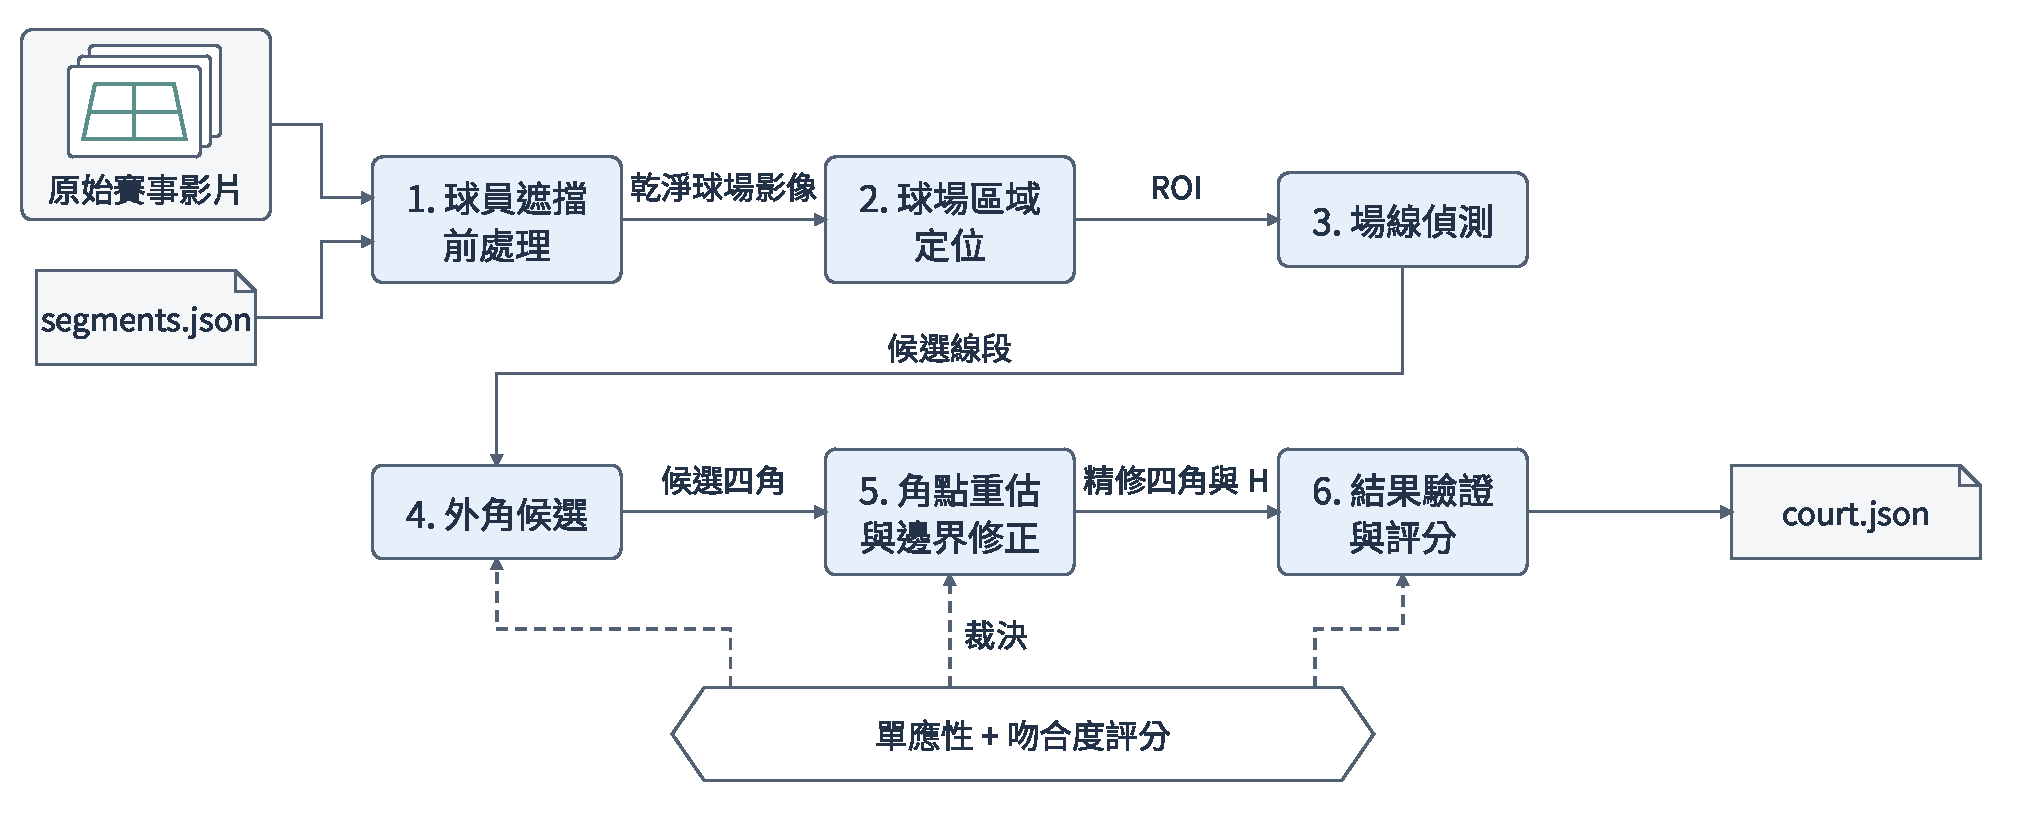
\includegraphics[scale=\flowscale]{court-detection.pdf}
  \caption{場地偵測處理流程}
  \label{fig:court-detection-flow}
\end{figure}

\subsubsection{球員遮擋前處理}

後續定位球場的主要訊號是顏色與場線，但轉播畫面中球員持續移動遮住場線與色塊，單張影格會使線條斷裂。本步驟要產生一張不含球員與短時雜訊的乾淨球場影像。機位固定時，球場在每張影格的同一座標都呈現相同顏色，唯有球員經過的少數影格例外，故對每個座標取多影格像素值的中位數，佔多數的球場顏色留下、屬於少數的球員與雜訊被濾除（\figref{fig:composite-median}）：
\begin{equation}
  M(x,y) = \mathrm{median}\{I_1(x,y),\dots,I_K(x,y)\}
\end{equation}

\begin{figure}[H]
  \centering
  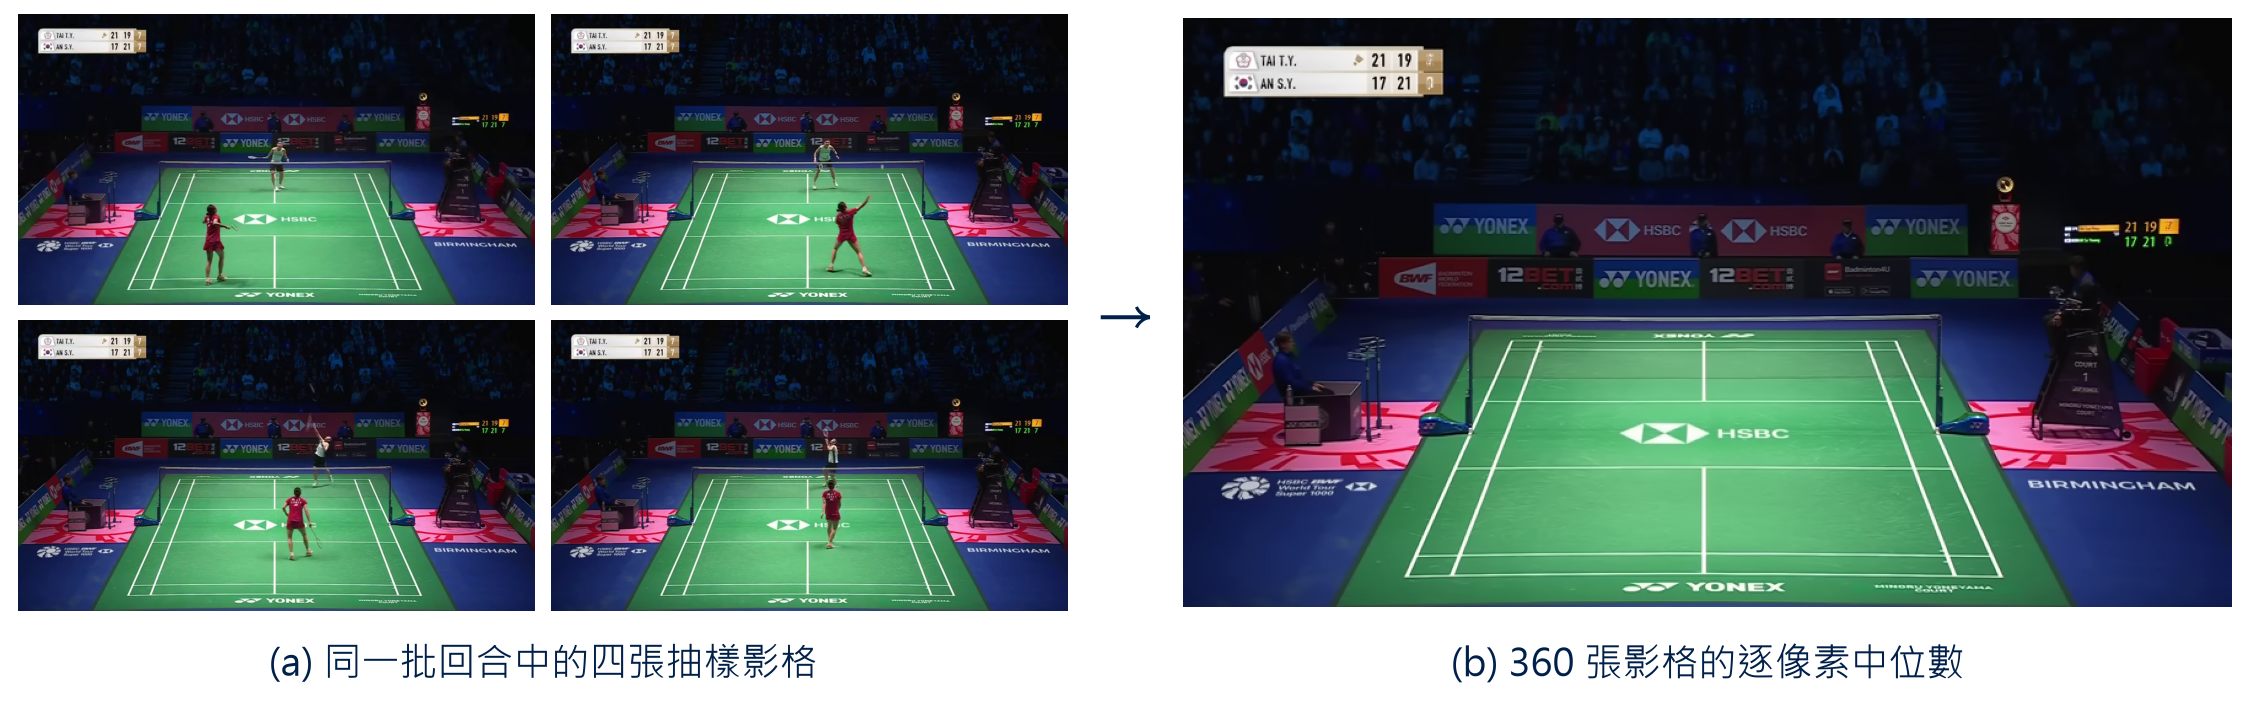
\includegraphics[width=\linewidth]{court_detection/composite_median.png}
  \caption{四張取樣影格與合成圖}
  \label{fig:composite-median}
\end{figure}

\subsubsection{球場區域定位}

本步驟要圈出球場在畫面中的大概範圍，好把範圍外的線段擋在後續場線偵測之外。實測對整張畫面掃描會得到近 200 條線段，真正屬於球場的只有 12 條（\figref{fig:mask-scope}）。

\begin{figure}[H]
  \centering
  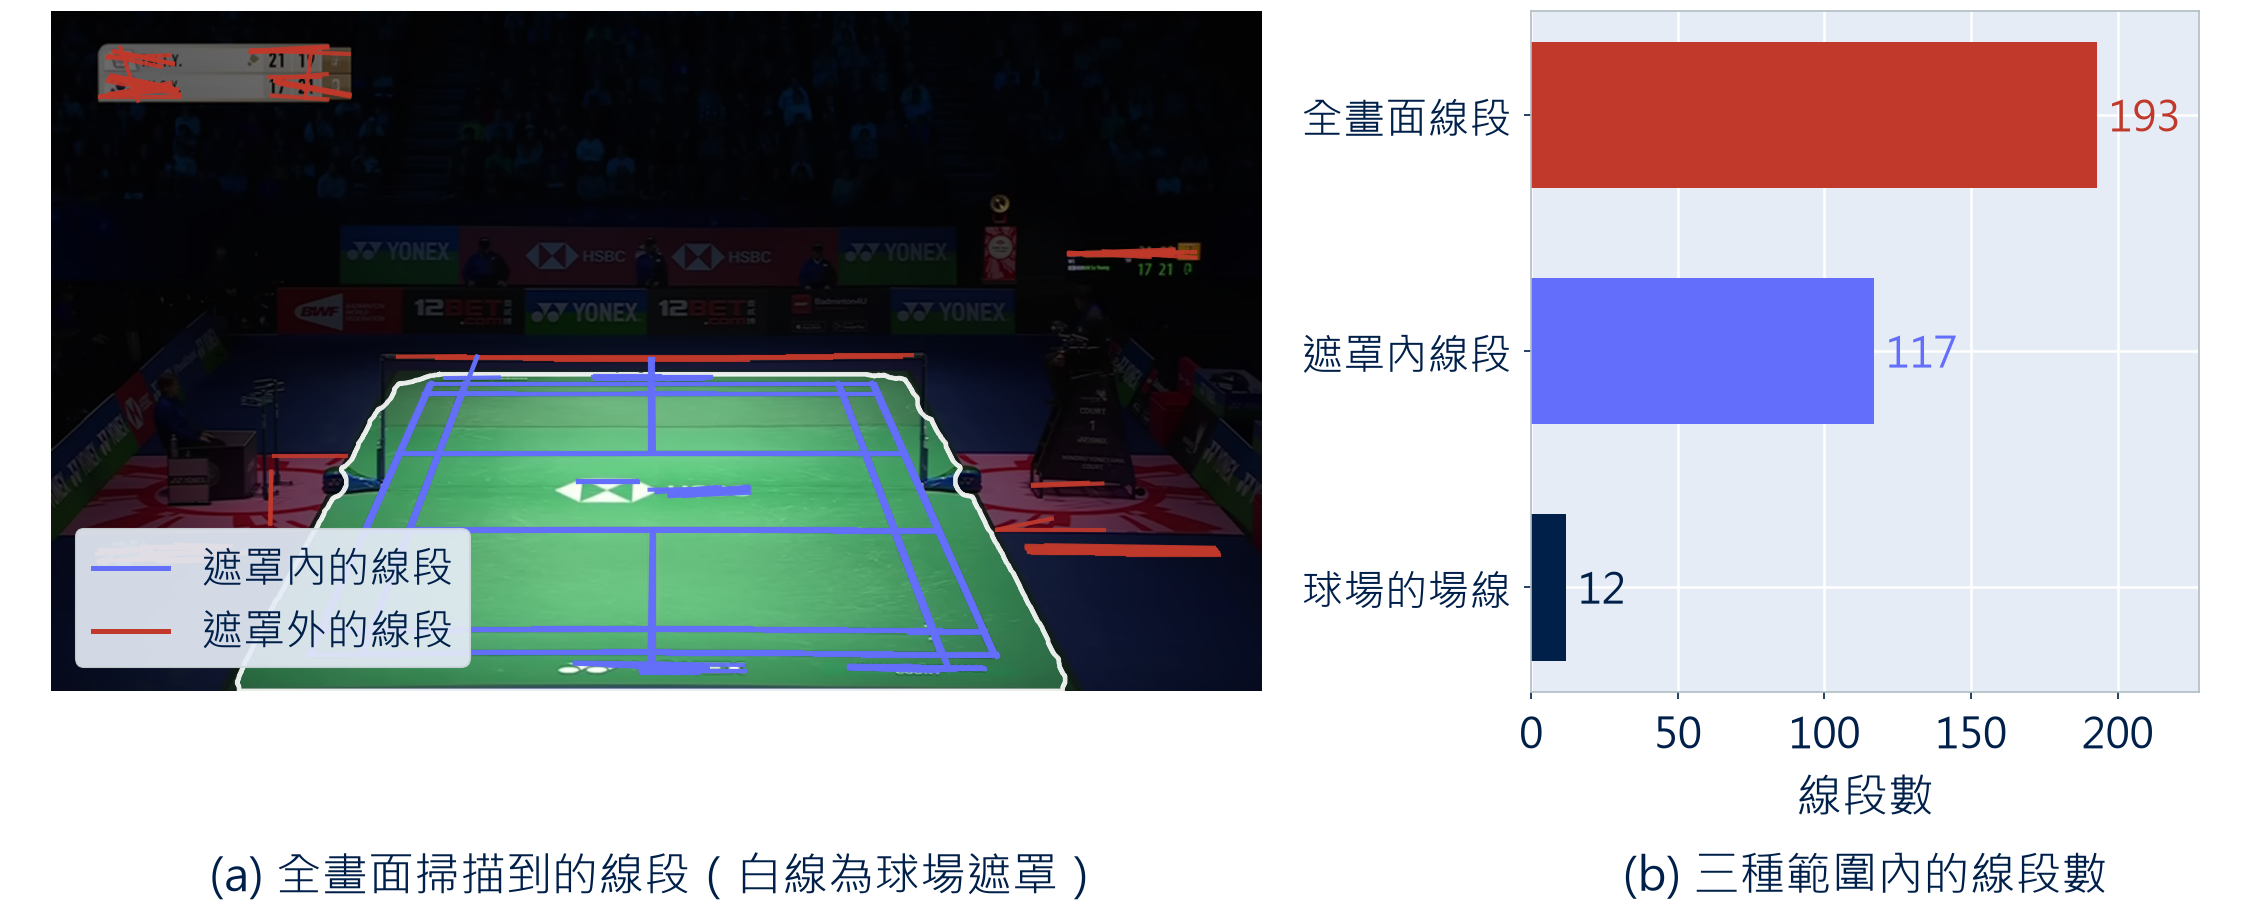
\includegraphics[width=\linewidth]{court_detection/mask_scope.png}
  \caption{全畫面掃描到的線段，與落在球場遮罩內的部分}
  \label{fig:mask-scope}
\end{figure}

分離球場與周邊地板的明顯特徵是顏色，但球場顏色本身未知。做法是在畫面中央偏下取一塊由機位假設保證落在場內的區域 $S$，取其像素在 Lab 色度（a、b）通道的中位數作為球場參考色 $\mathbf{c}$，任一像素的色度與 $\mathbf{c}$ 的距離小於門檻 $\tau_c$ 即判為球場：
\begin{gather}
  \mathbf{c} = \big(\mathrm{median}_{S}\,a,\ \mathrm{median}_{S}\,b\big), \qquad \tau_c = \max\!\Big(18,\ 3 \cdot \tfrac{\sigma_a + \sigma_b}{2}\Big) \\
  C(x,y) = \big[\,\lVert\,(a(x,y),\,b(x,y)) - \mathbf{c}\,\rVert < \tau_c\,\big]
\end{gather}
其中 $\sigma_a,\sigma_b$ 為 $S$ 在兩色度通道的標準差。捨棄亮度通道使光照與陰影不進入判斷。用中位數以避免取樣區塊內的像素影響門檻。門檻取 $3\sigma$ 使其隨取樣塊自身的顏色離散程度放寬，下限 18 則用以容忍過於平滑的場地（\figref{fig:lab-chroma}）。

\begin{figure}[H]
  \centering
  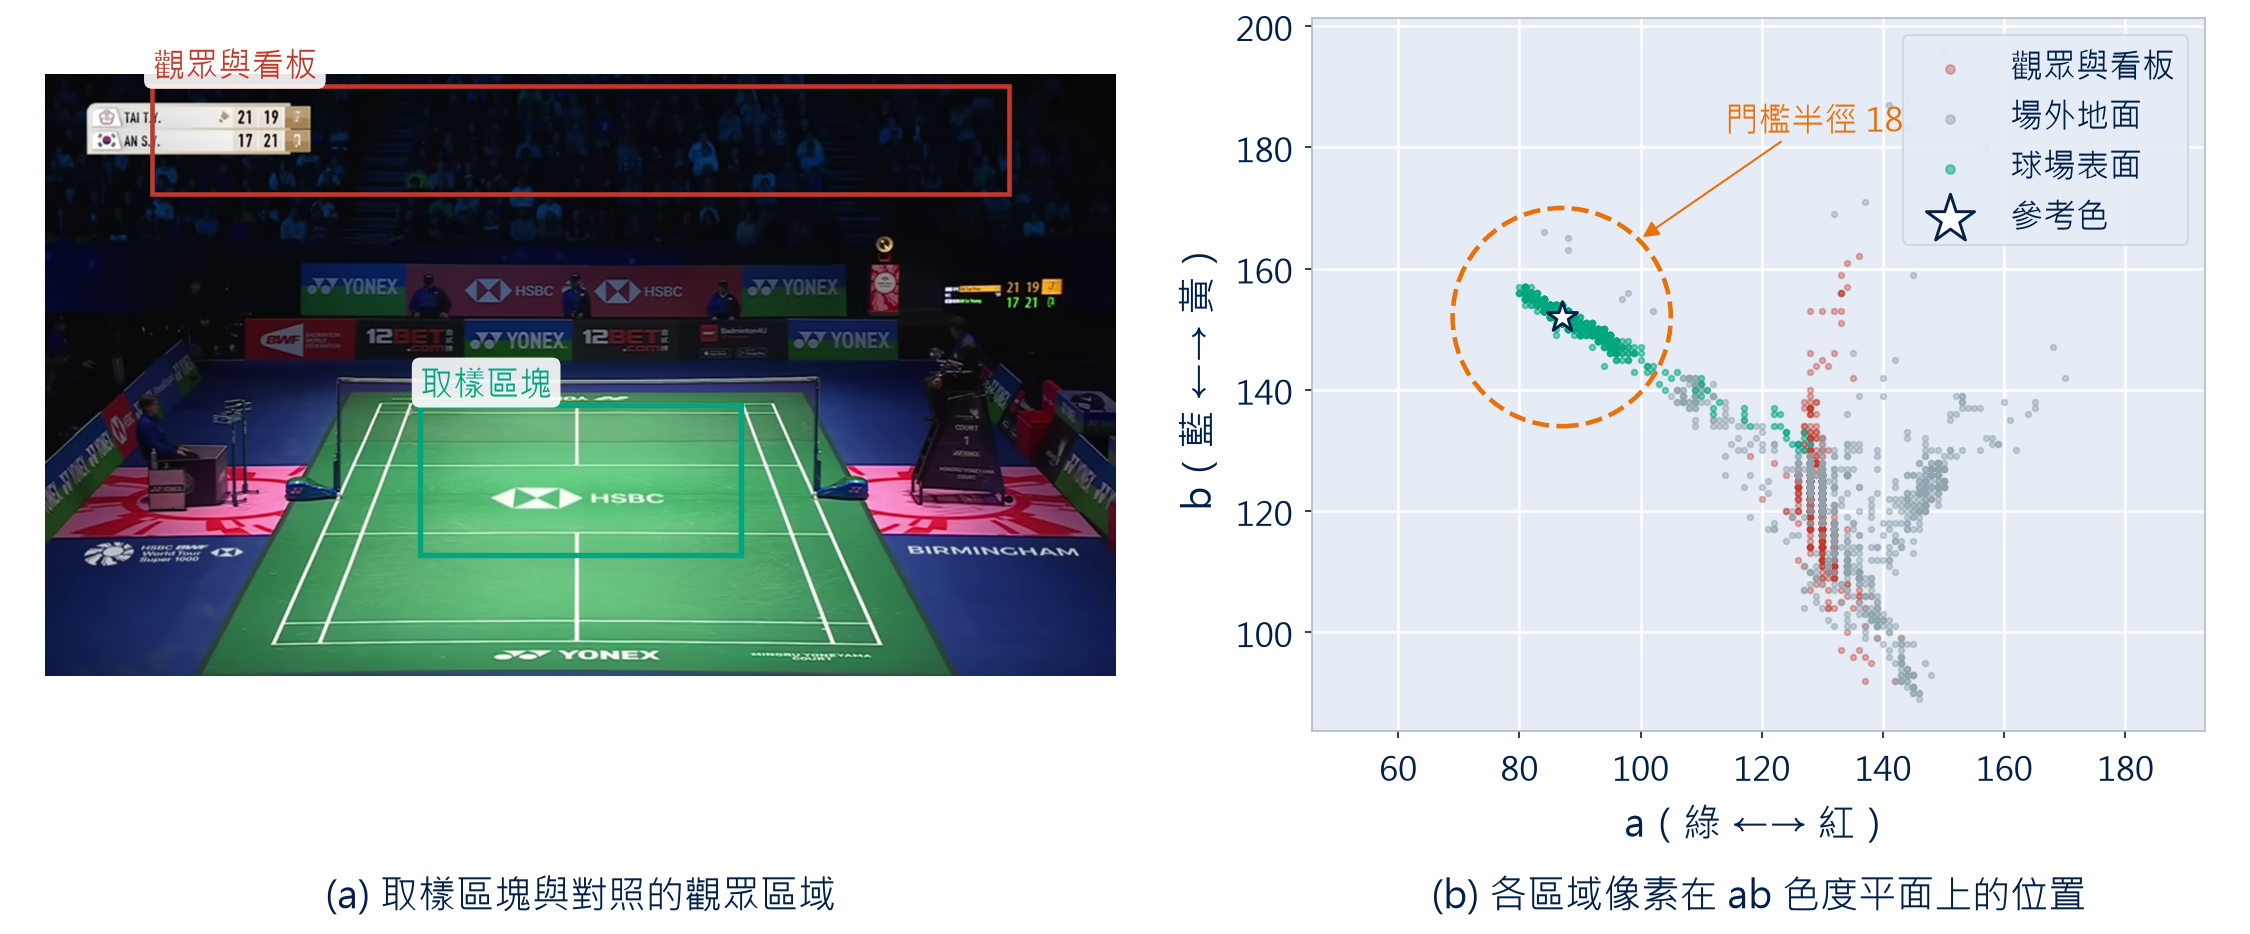
\includegraphics[width=\linewidth]{court_detection/lab_chroma.png}
  \caption{取樣區塊、參考色與門檻的判定}
  \label{fig:lab-chroma}
\end{figure}

上述門檻得到的是逐像素獨立的判斷，還不是一塊完整區域。白色場線把場地切成數塊，雜訊與反光留下零星破洞。模組以形態學運算補洞去雜點、取面積最大的連通區域、再自畫面左上角向內填充背景，把內部空洞併回球場（\figref{fig:morphology}）。

\begin{figure}[H]
  \centering
  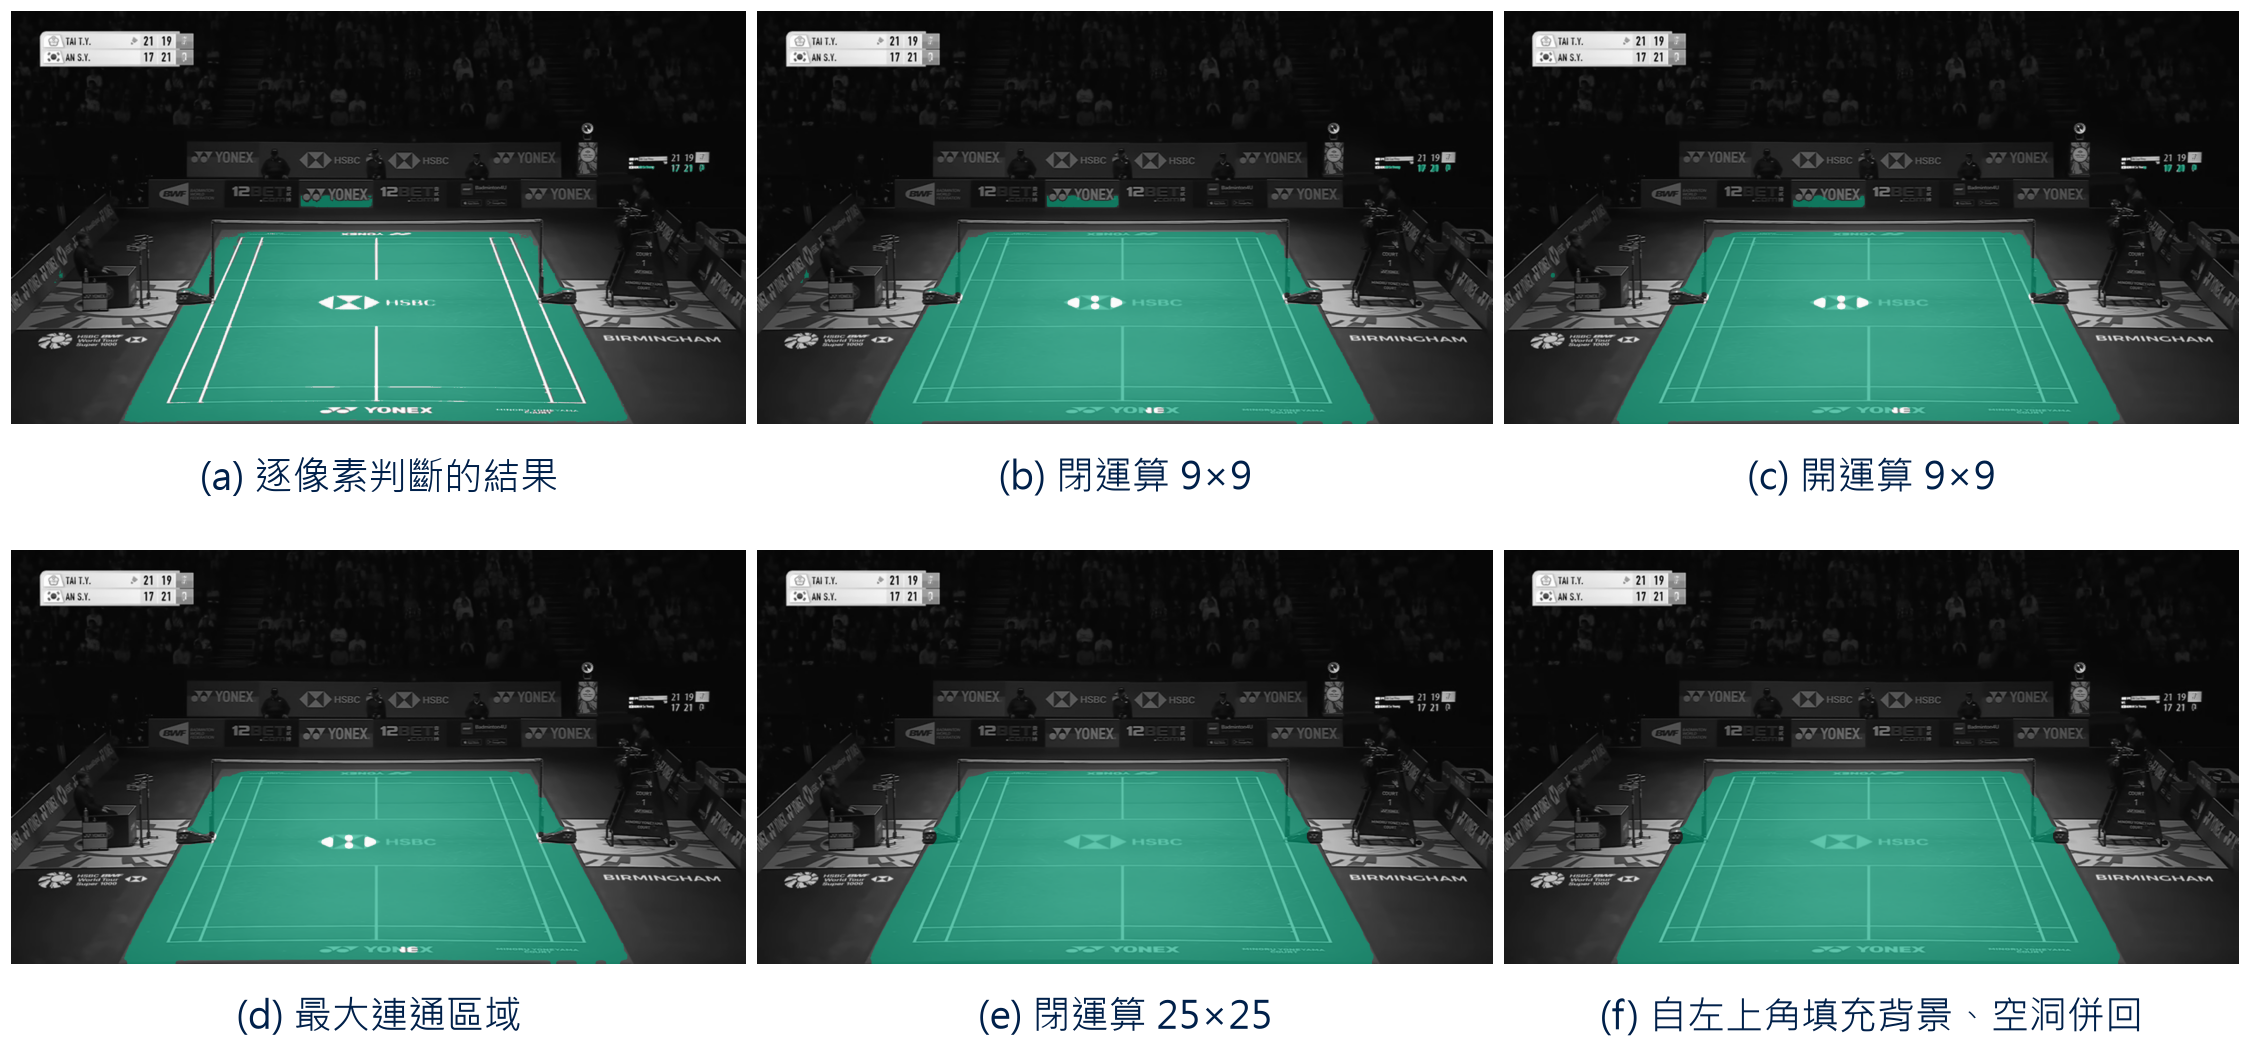
\includegraphics[width=\linewidth]{court_detection/morphology.png}
  \caption{形態學清理、最大連通區域與空洞填補各階段的遮罩變化}
  \label{fig:morphology}
\end{figure}

本步驟實際產生的不只一張遮罩。除上述色度版本外，另備一個紋理版本，在色度條件之外再加一道局部亮度標準差門檻，只留下平滑區域，用以濾掉與場地同色卻花紋雜亂的地面贊助商圖樣（\figref{fig:texture-gate}）。另有一個低色度版本，在整體畫面色度過低、色度判準失效時改以亮度相似度取代色度。這些版本不互相取代，而是一併往下送，構成後續多假設並行的二至三組遮罩。

\begin{figure}[H]
  \centering
  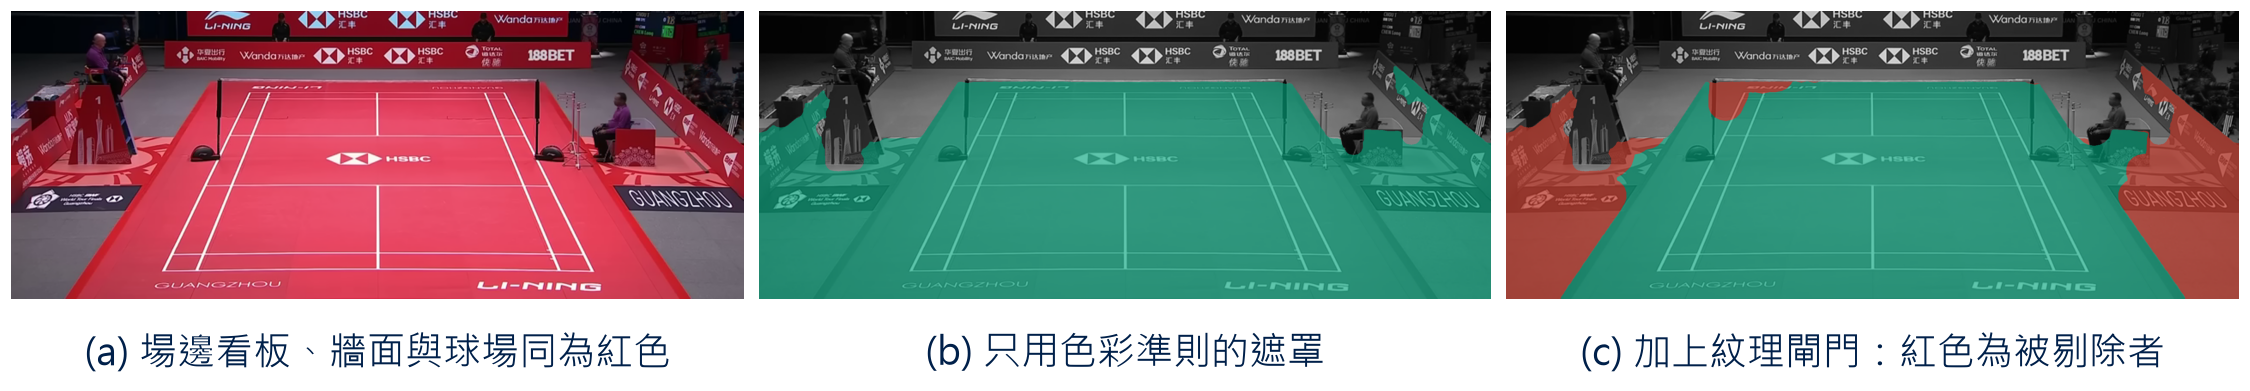
\includegraphics[width=\linewidth]{court_detection/texture_gate.png}
  \caption{場邊看板與球場同色時，紋理版本剔除色度版本誤納的區域}
  \label{fig:texture-gate}
\end{figure}

\subsubsection{場線偵測}

本步驟要在前一步的遮罩範圍內找出球場線，過程分四段，取出屬於線的像素、把像素組織成線段、濾除不屬於球場的線段、合併接近的線段。

取線像素不靠色彩，轉播素材的曝光與白平衡各異、場線的絕對色值並不固定。使用局部亮度突起，一個像素若比水平（或垂直）方向兩側都亮出門檻 $\tau$，即屬近垂直（或近水平）的線像素，$P_h$、$P_v$ 取聯集，比較距離 $d$ 須大於線寬（\figref{fig:line-pixels}）：
\begin{gather}
  P_h(x,y) = \big[\,G(x,y)-G(x-d,y) > \tau\,\big] \wedge \big[\,G(x,y)-G(x+d,y) > \tau\,\big] \\
  P_v(x,y) = \big[\,G(x,y)-G(x,y-d) > \tau\,\big] \wedge \big[\,G(x,y)-G(x,y+d) > \tau\,\big]
\end{gather}

\begin{figure}[H]
  \centering
  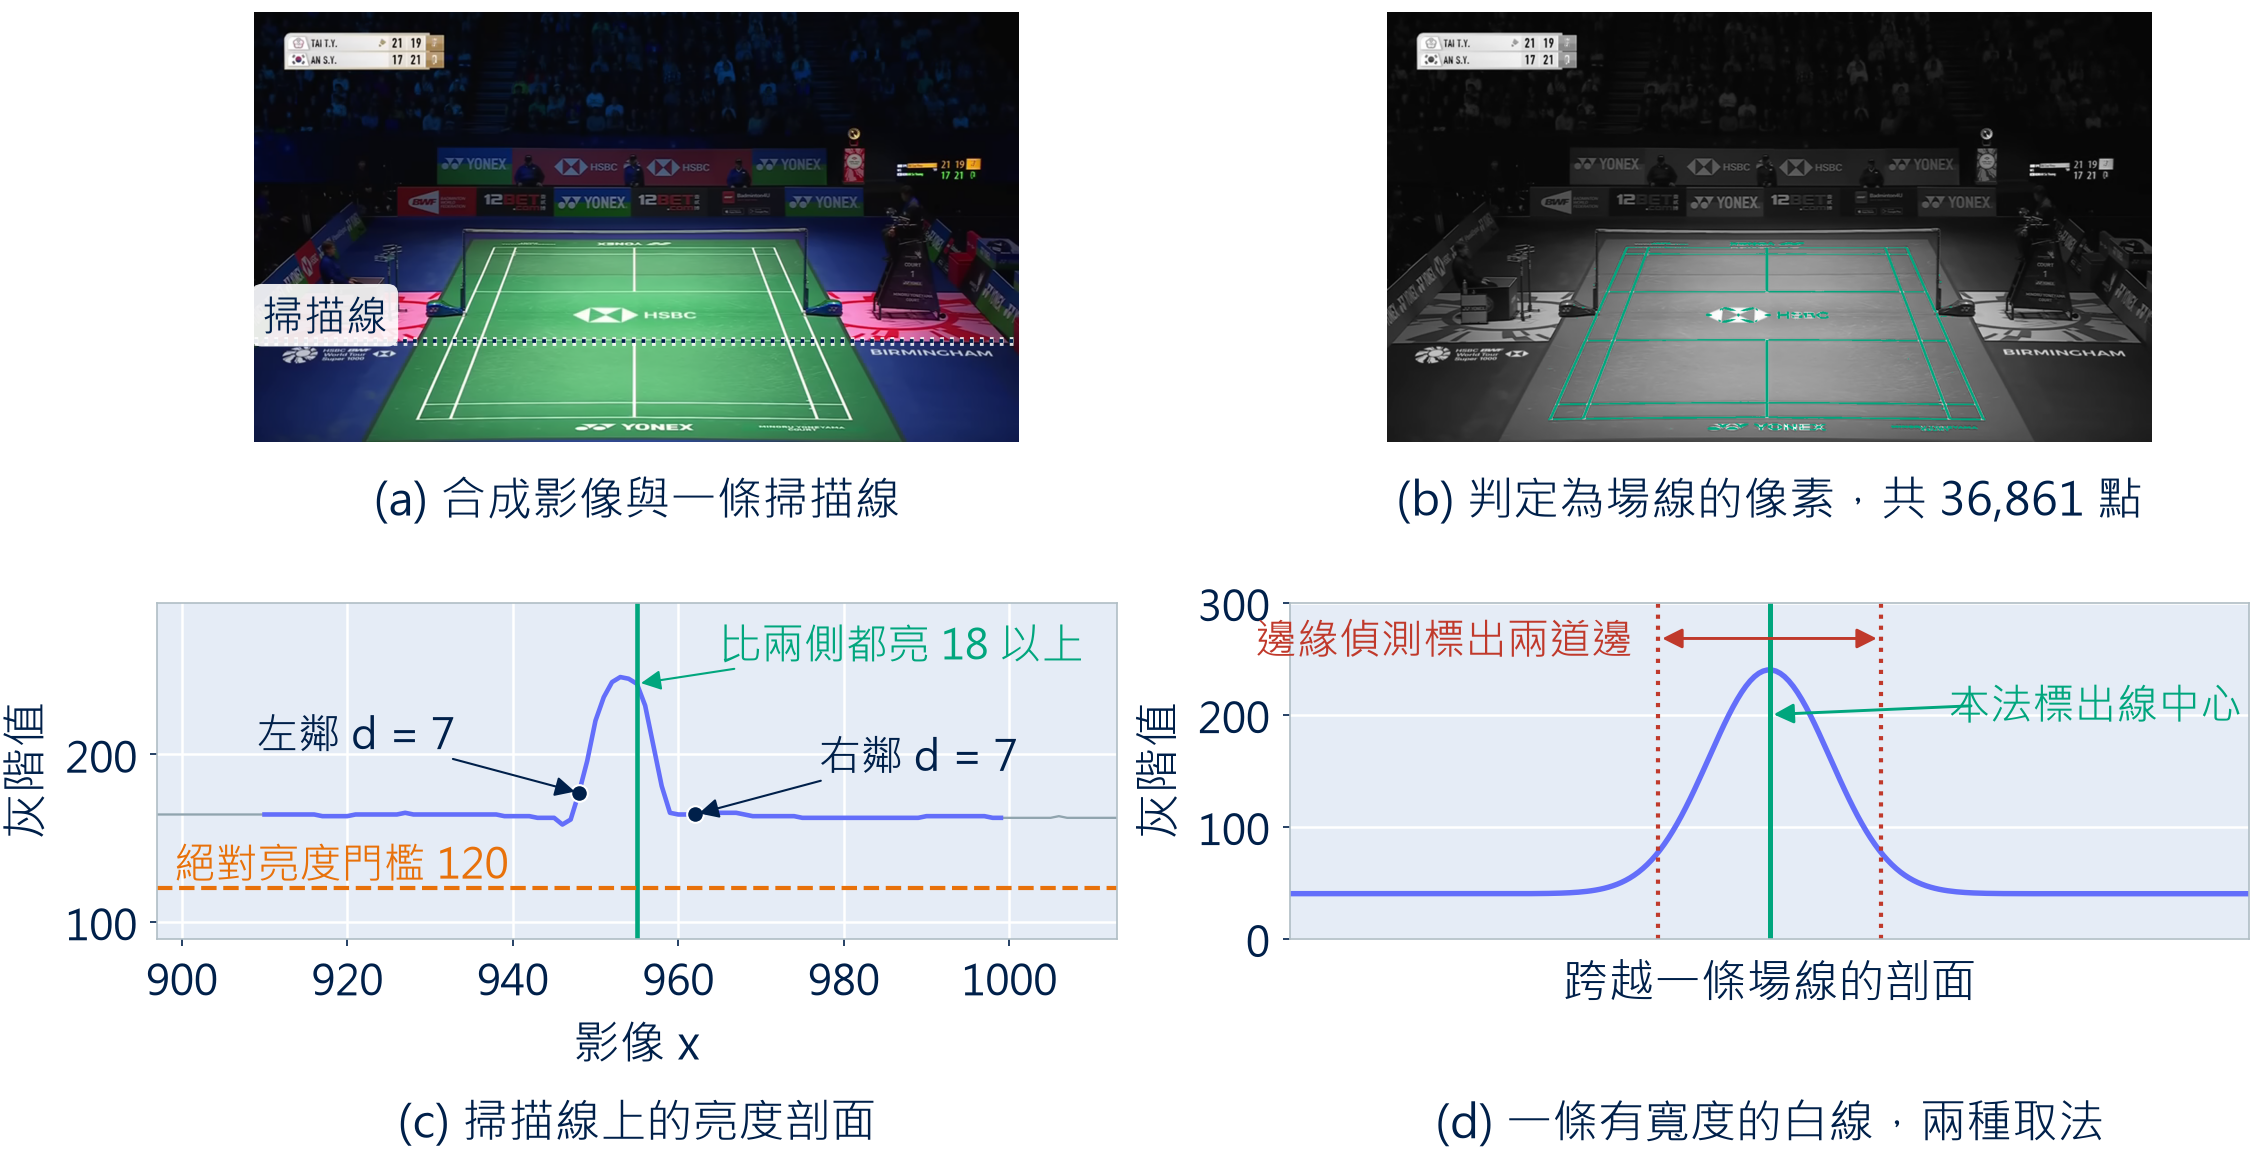
\includegraphics[width=\linewidth]{court_detection/line_pixels.png}
  \caption{局部亮度突起與場線像素的萃取結果}
  \label{fig:line-pixels}
\end{figure}

上一步的輸出是散落的像素，以機率霍夫轉換（PPHT，\texttt{cv2.HoughLinesP}）把共線者組織成線段（\figref{fig:hough-families}）。場線常因球員殘影、地面反光與遮罩侵蝕而斷開，霍夫轉換靠投票決定共線性、不依賴像素連通，能跨越這些缺口。

\begin{figure}[H]
  \centering
  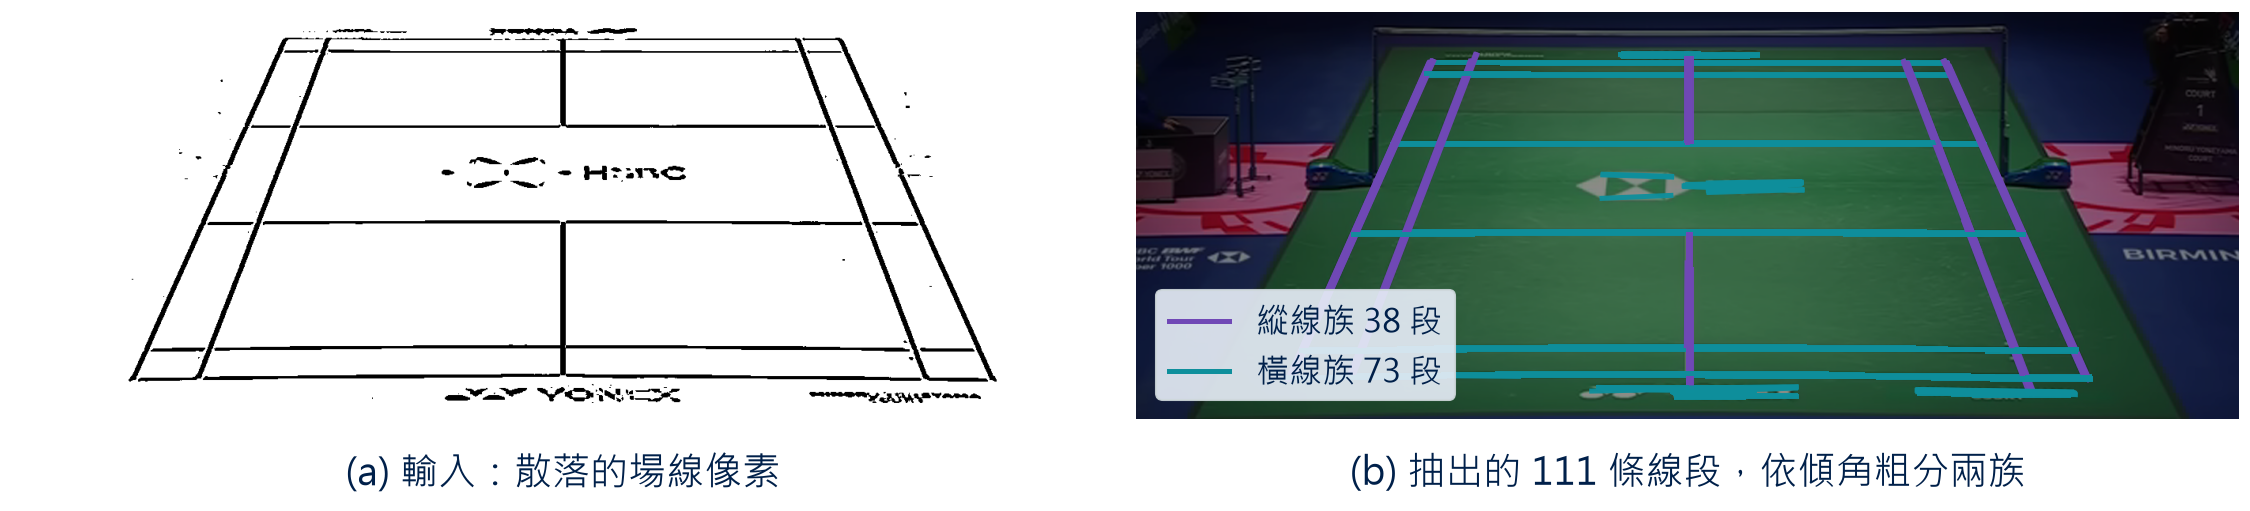
\includegraphics[width=\linewidth]{court_detection/hough_families.png}
  \caption{霍夫線段與兩族的角度粗分}
  \label{fig:hough-families}
\end{figure}

粗分後仍混有地面贊助商圖樣等非球場線段，以透視幾何篩選。球場的 12 條線分屬兩組平行線，在畫面上各自通過一個消失點。找消失點是離群比例可能很高的穩健估計問題，採 RANSAC，隨機取兩條線段、以交點為候選消失點，統計族內有多少線段方向指向它（以線段長度加權），重複數百次取支持度最高者（\figref{fig:vp-ransac}）。

\begin{figure}[H]
  \centering
  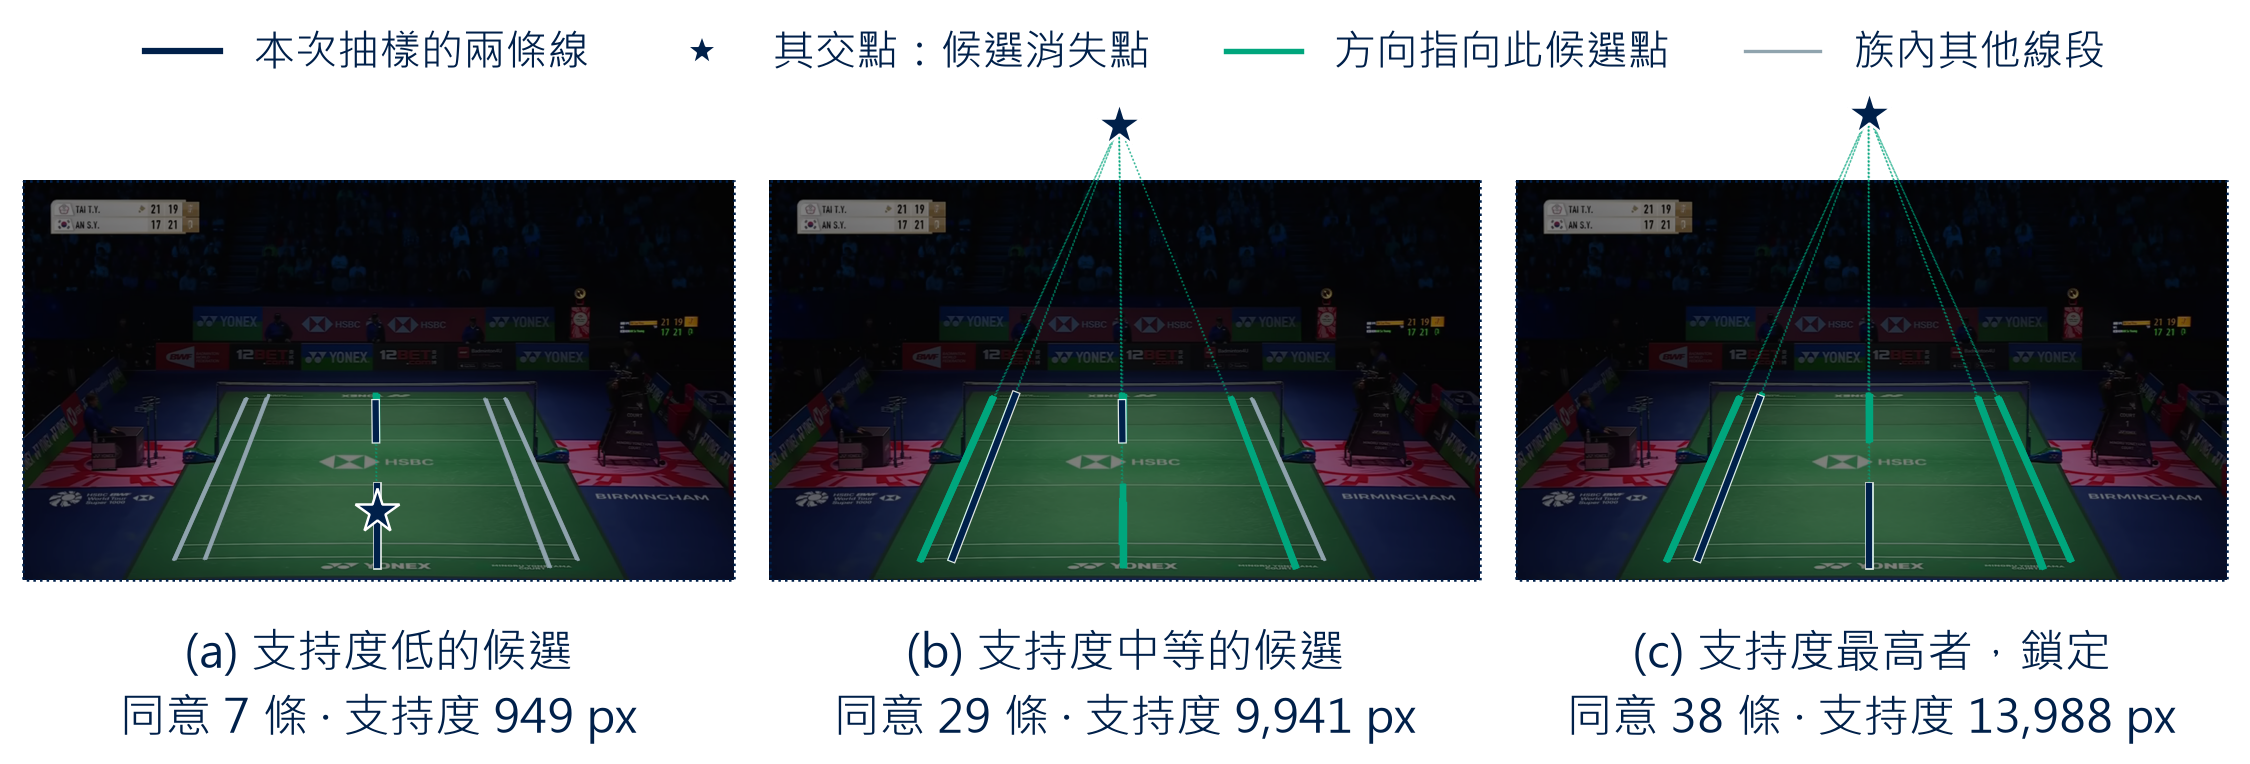
\includegraphics[width=\linewidth]{court_detection/vp_ransac.png}
  \caption{消失點 RANSAC 三次抽樣的候選點與其支持度}
  \label{fig:vp-ransac}
\end{figure}

球網遮擋常把一條球場線拆成方向略有出入的數段，同一條物理線會以不同位置重複參與運算，故先合併。同族線段方向相近、只在垂直於該方向的位置上分開，取一條參考線把每條線段化為一維位置，位置相近者歸為一簇，每簇以最小平方擬合出一條代表線。數百條線段因此收斂成十餘條物理線，既去除重複，也把後續窮舉的組合數壓到可行範圍（\figref{fig:line-merge}）。

\begin{figure}[H]
  \centering
  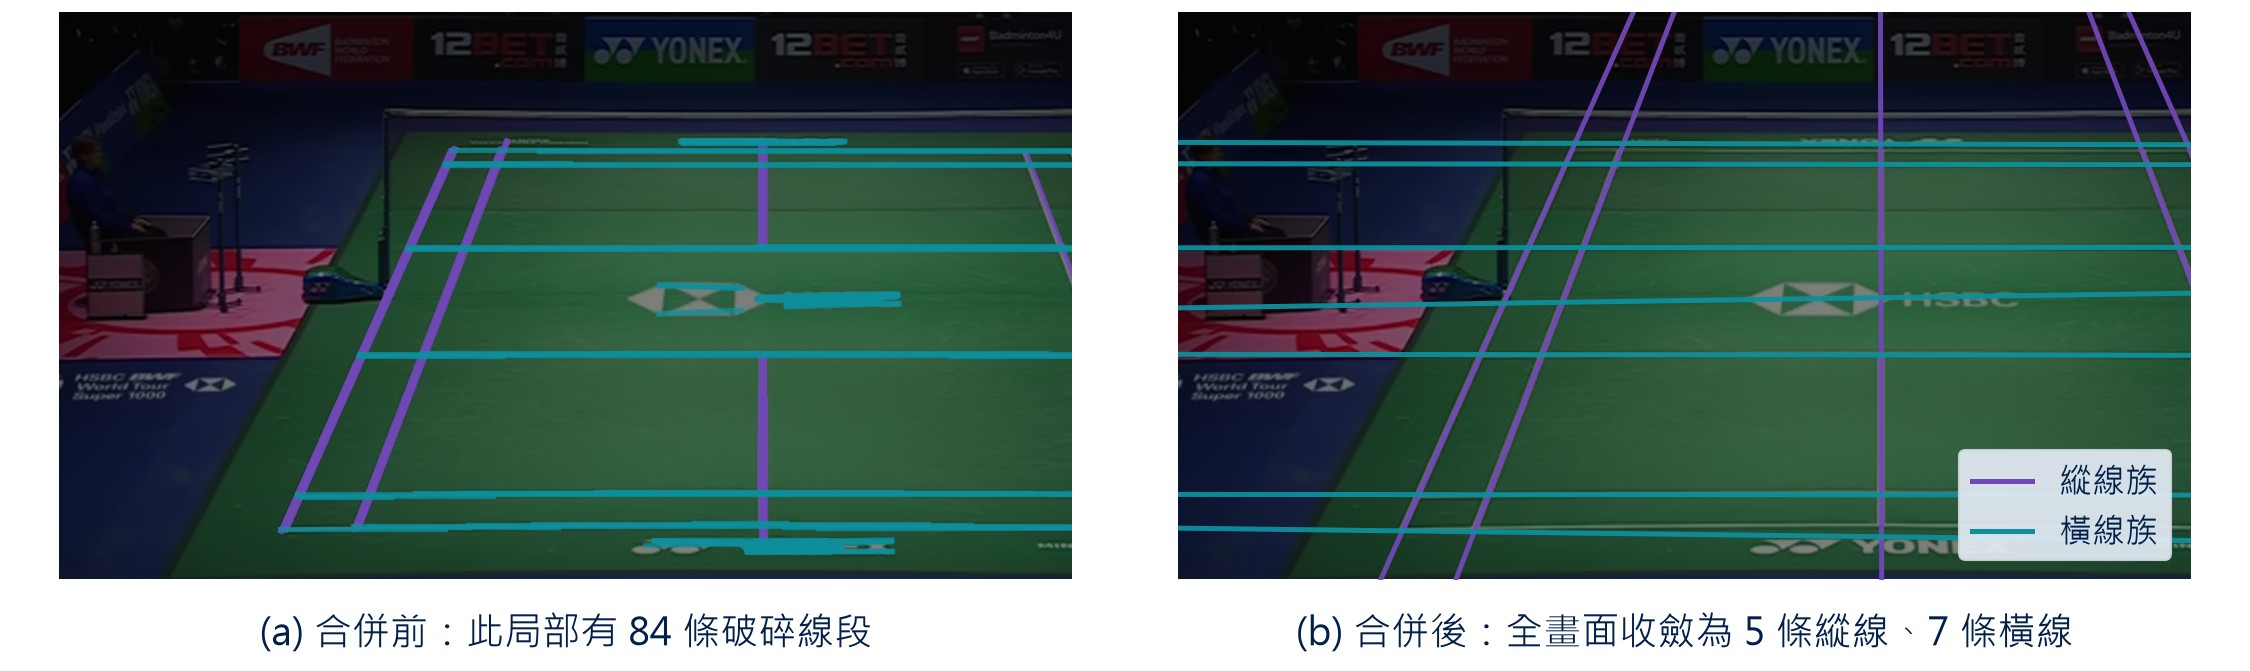
\includegraphics[width=\linewidth]{court_detection/line_merge.png}
  \caption{同族線段合併的前後對比}
  \label{fig:line-merge}
\end{figure}

\subsubsection{單應性與吻合度評分}

本步驟解決「如何由四角解出單應性、如何量化一組四角的好壞」的問題。

羽球場的尺寸與 12 條場線位置皆為已知常數，因此可預先建立球場模型座標：5 條縱線對應固定的 $x$ 值，7 條橫線對應固定的 $y$ 值。將模型四角與影像中偵測到的四角建立對應後，即可用 DLT 解出單應性 $\mathrm{H}$，再由 $\mathrm{H}$ 將模型中的 12 條場線與 16 個交點一併投影至影像。

DLT 對趨近退化的輸入不會報錯，仍會得出病態的 $\mathrm{H}$，故對每個 $\mathrm{H}$ 加設合法性檢查：四角須為有限值、不超出畫面、不退化成細條、近端底線不短於遠端（\figref{fig:valid-h}）。此檢查貫穿後續所有產生 $\mathrm{H}$ 的階段。

\begin{figure}[H]
  \centering
  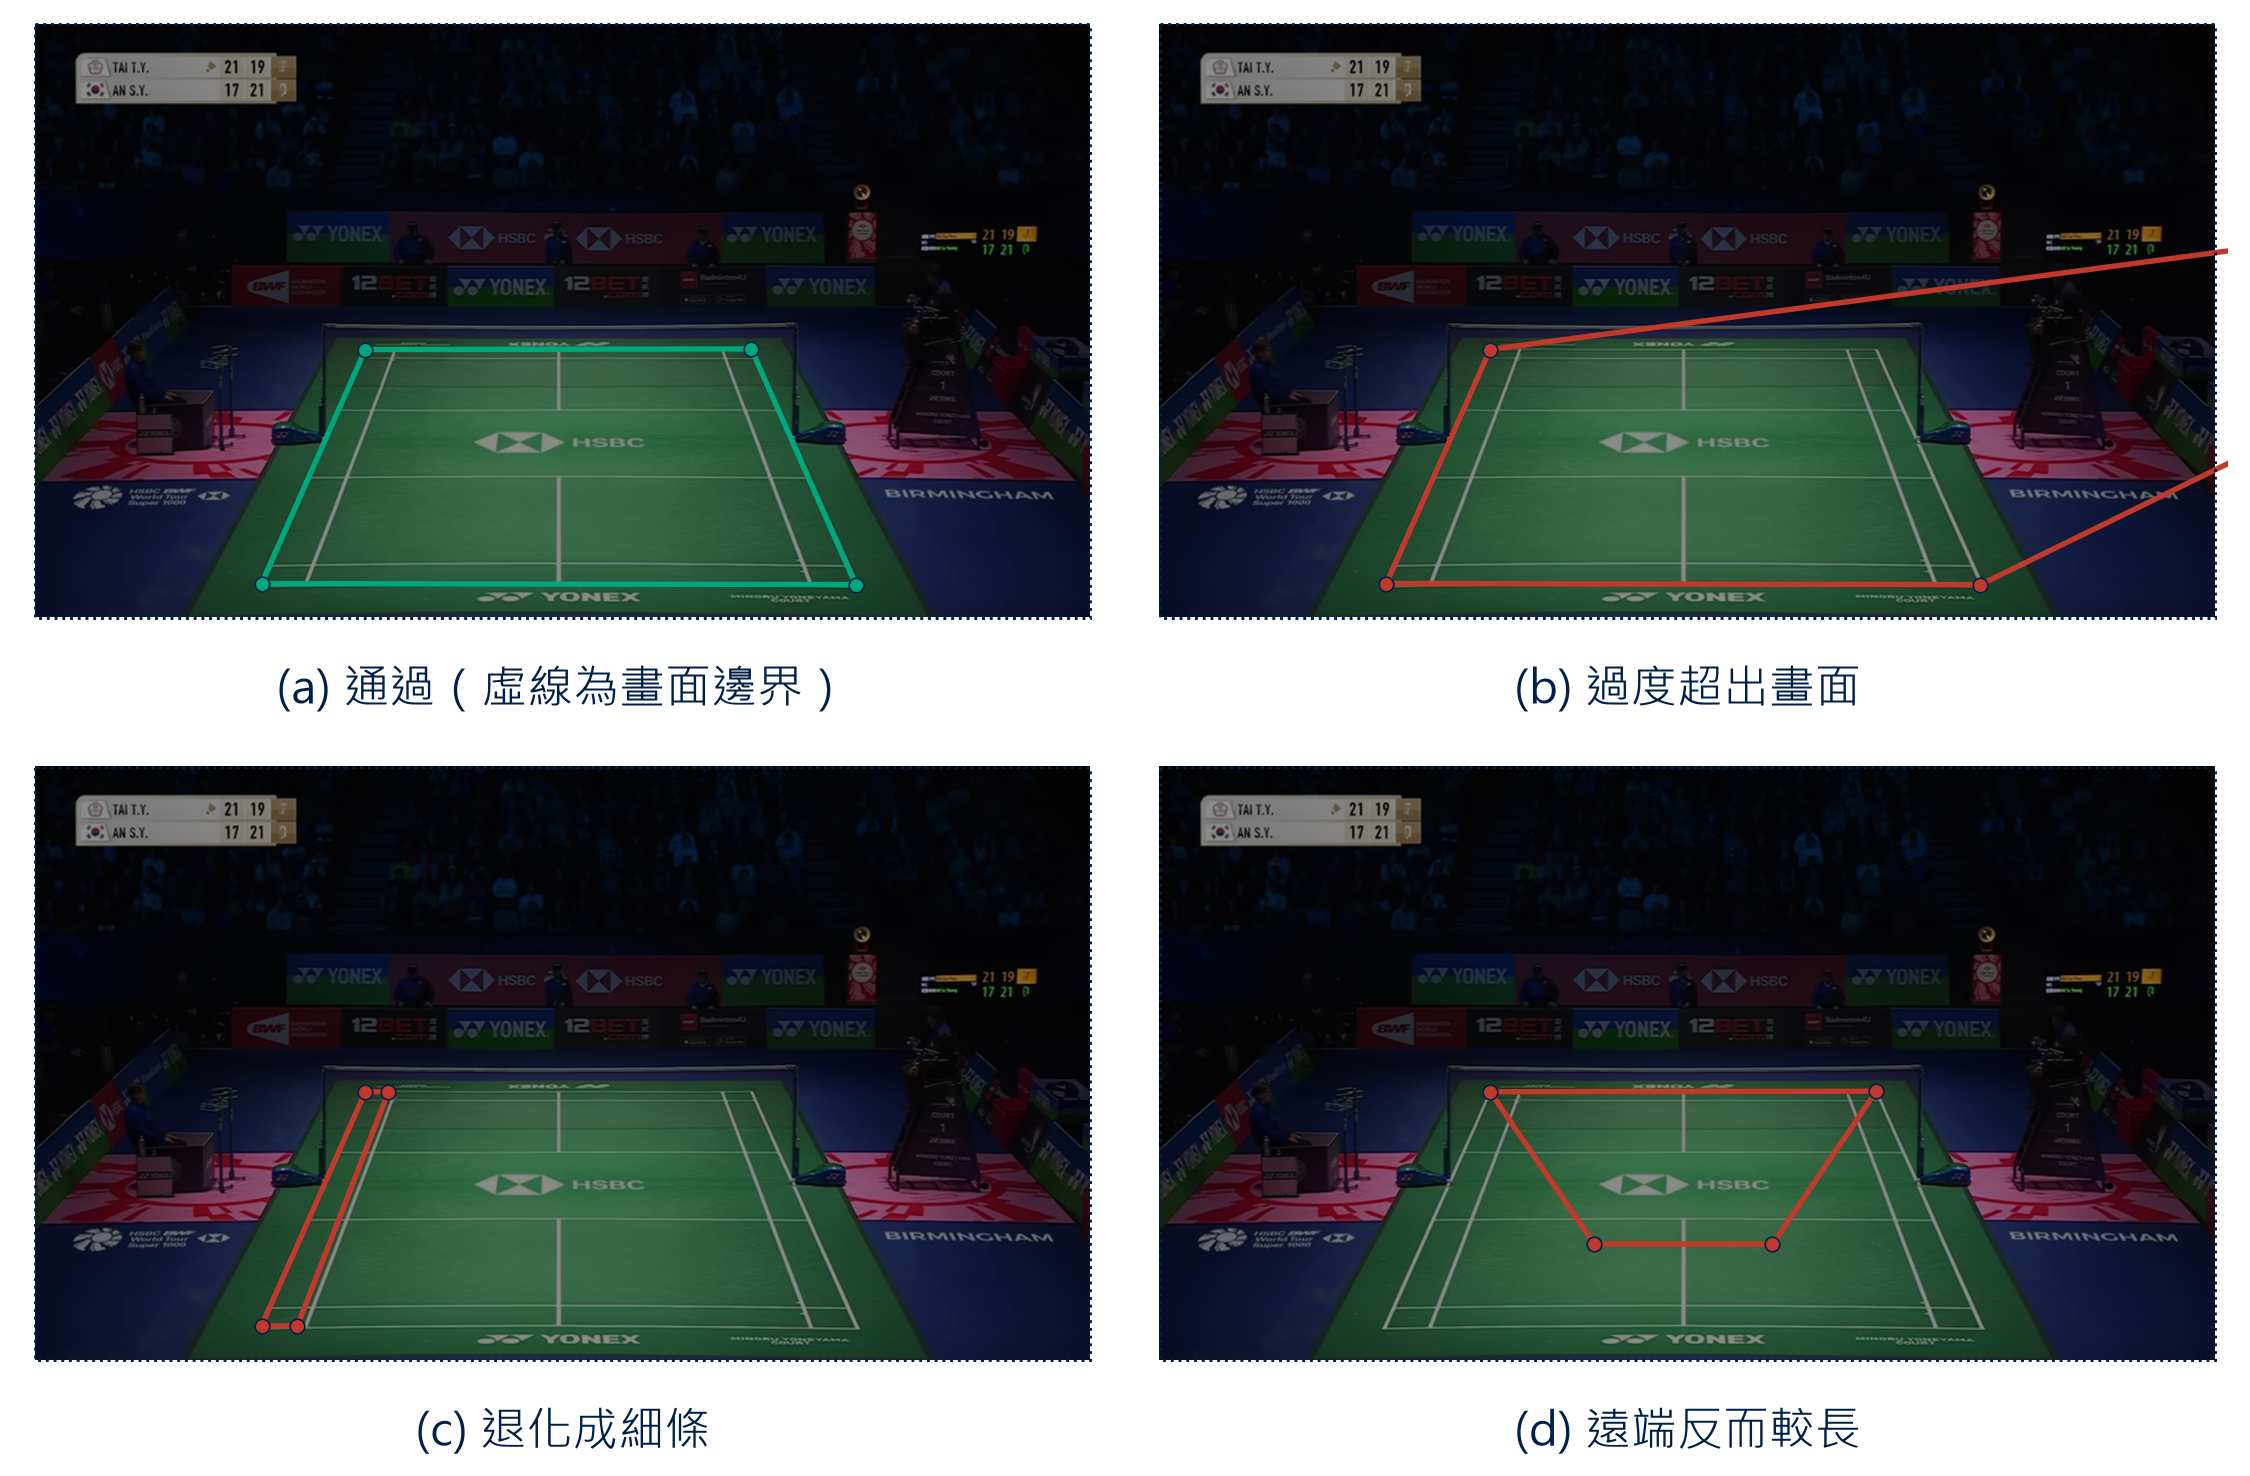
\includegraphics[width=\linewidth]{court_detection/valid_h.png}
  \caption{合法性檢查}
  \label{fig:valid-h}
\end{figure}

吻合度評分衡量 $\mathrm{H}$ 推出的網格與畫面上實際偵測到的場線像素有多吻合。單條線的覆蓋率定義為：沿線等距取若干點、投影到影像，落在最近場線像素容差（4 像素）內的比例（\figref{fig:distance-transform}）。總評分取「貼合度」與「廣度」兩項相乘：
\begin{equation}
  S = \underbrace{\frac{1}{12}\sum_{k=1}^{12}\mathrm{cov}_k}_{\text{貼合度}} \times \underbrace{\frac{1}{12}\big\lvert\{\,k : \mathrm{cov}_k > 0.3\,\}\big\rvert}_{\text{廣度}}
  \label{eq:court-score}
\end{equation}
此評分是整個場地偵測判斷好壞的統一依據，後續的候選選擇與邊界修正都以它裁決。

\begin{figure}[H]
  \centering
  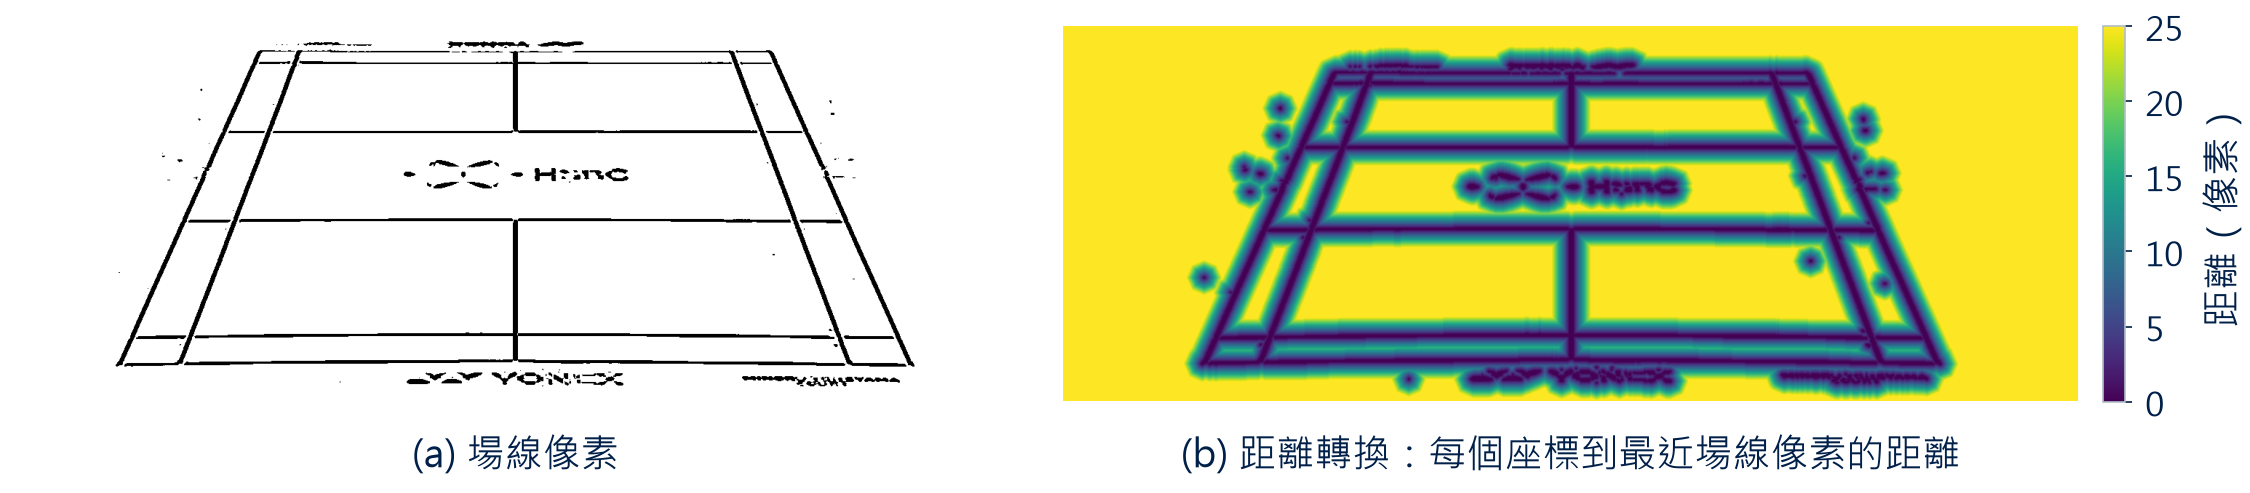
\includegraphics[width=\linewidth]{court_detection/distance_transform.png}
  \caption{場線像素與其距離轉換圖}
  \label{fig:distance-transform}
\end{figure}

\subsubsection{外角候選}

四角須由偵測到的線或遮罩推導，任一種推導都有其失效條件，故本模組並行三種來源、各給一組候選，三者的失效條件互不重疊。

\textbf{網格枚舉（主要方法）：}從候選縱線任取兩條作左右邊界、橫線任取兩條作上下邊界，四線相交得一組四角，枚舉所有 $\binom{10}{2}\times\binom{12}{2}=2970$ 組合，取 12 線網格吻合度最高者（\figref{fig:grid-search}）。穩健的關鍵在於以最可靠的內部線反推最不可靠的外角，等於讓發球線與中線一起投票決定四角。

\begin{figure}[H]
  \centering
  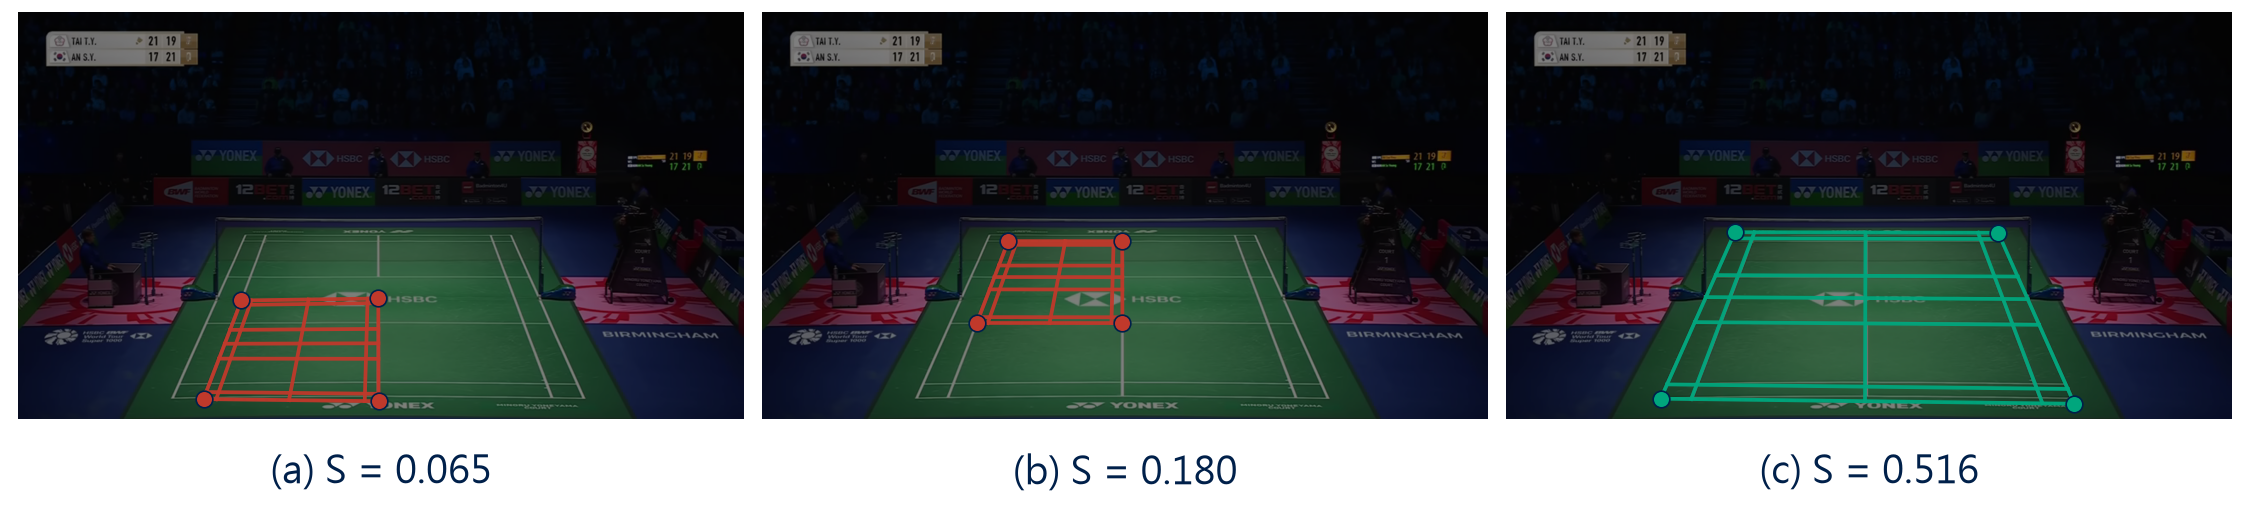
\includegraphics[width=\linewidth]{court_detection/grid_search.png}
  \caption{網格枚舉的候選與其吻合度評分}
  \label{fig:grid-search}
\end{figure}

\textbf{極端線相交：}在兩族中各取最外側的兩條線相交得四角，最直接，但要求那四條極端線全部正確，而外緣線最難偵測，故僅作第二來源。它的失效條件與網格枚舉不同，能在枚舉搜尋空間無正解時補位。

\textbf{遮罩凸包：}改用遮罩形狀，取面積最大的外輪廓、求凸包並簡化為多邊形，再由頂點座標的極值取出四角。它不需任何場線，但遮罩邊界經形態學處理與空洞填補、未必等於球場外緣，精度最低，僅在前兩者都產生不出合法 $\mathrm{H}$ 時作為備援。

\subsubsection{角點重估與邊界修正}

前一步的四角只由少數代表線相交而得，影像中大量場線像素尚未參與，本步驟用上全部線像素把結果調準，分兩階段。

\textbf{以 ICP 重估單應性：}難點在建立線像素與球場模型的對應，影像中場線因透視而方向各異，難以直接配對。利用前一步的近似 $\mathrm{H}$，把每個線像素反投影回球場座標，那裡的縱線是 $x$ 為定值、橫線是 $y$ 為定值的直線，量出該像素離哪條最近即建立對應。再用全部點對重解 $\mathrm{H}$、以新 $\mathrm{H}$ 更新對應，反覆逼近。點對數以千計，採 RANSAC 版本把配錯到相鄰線的像素當離群值排除，對應的距離門檻隨迭代由寬到窄（\figref{fig:icp}）。

\begin{figure}[H]
  \centering
  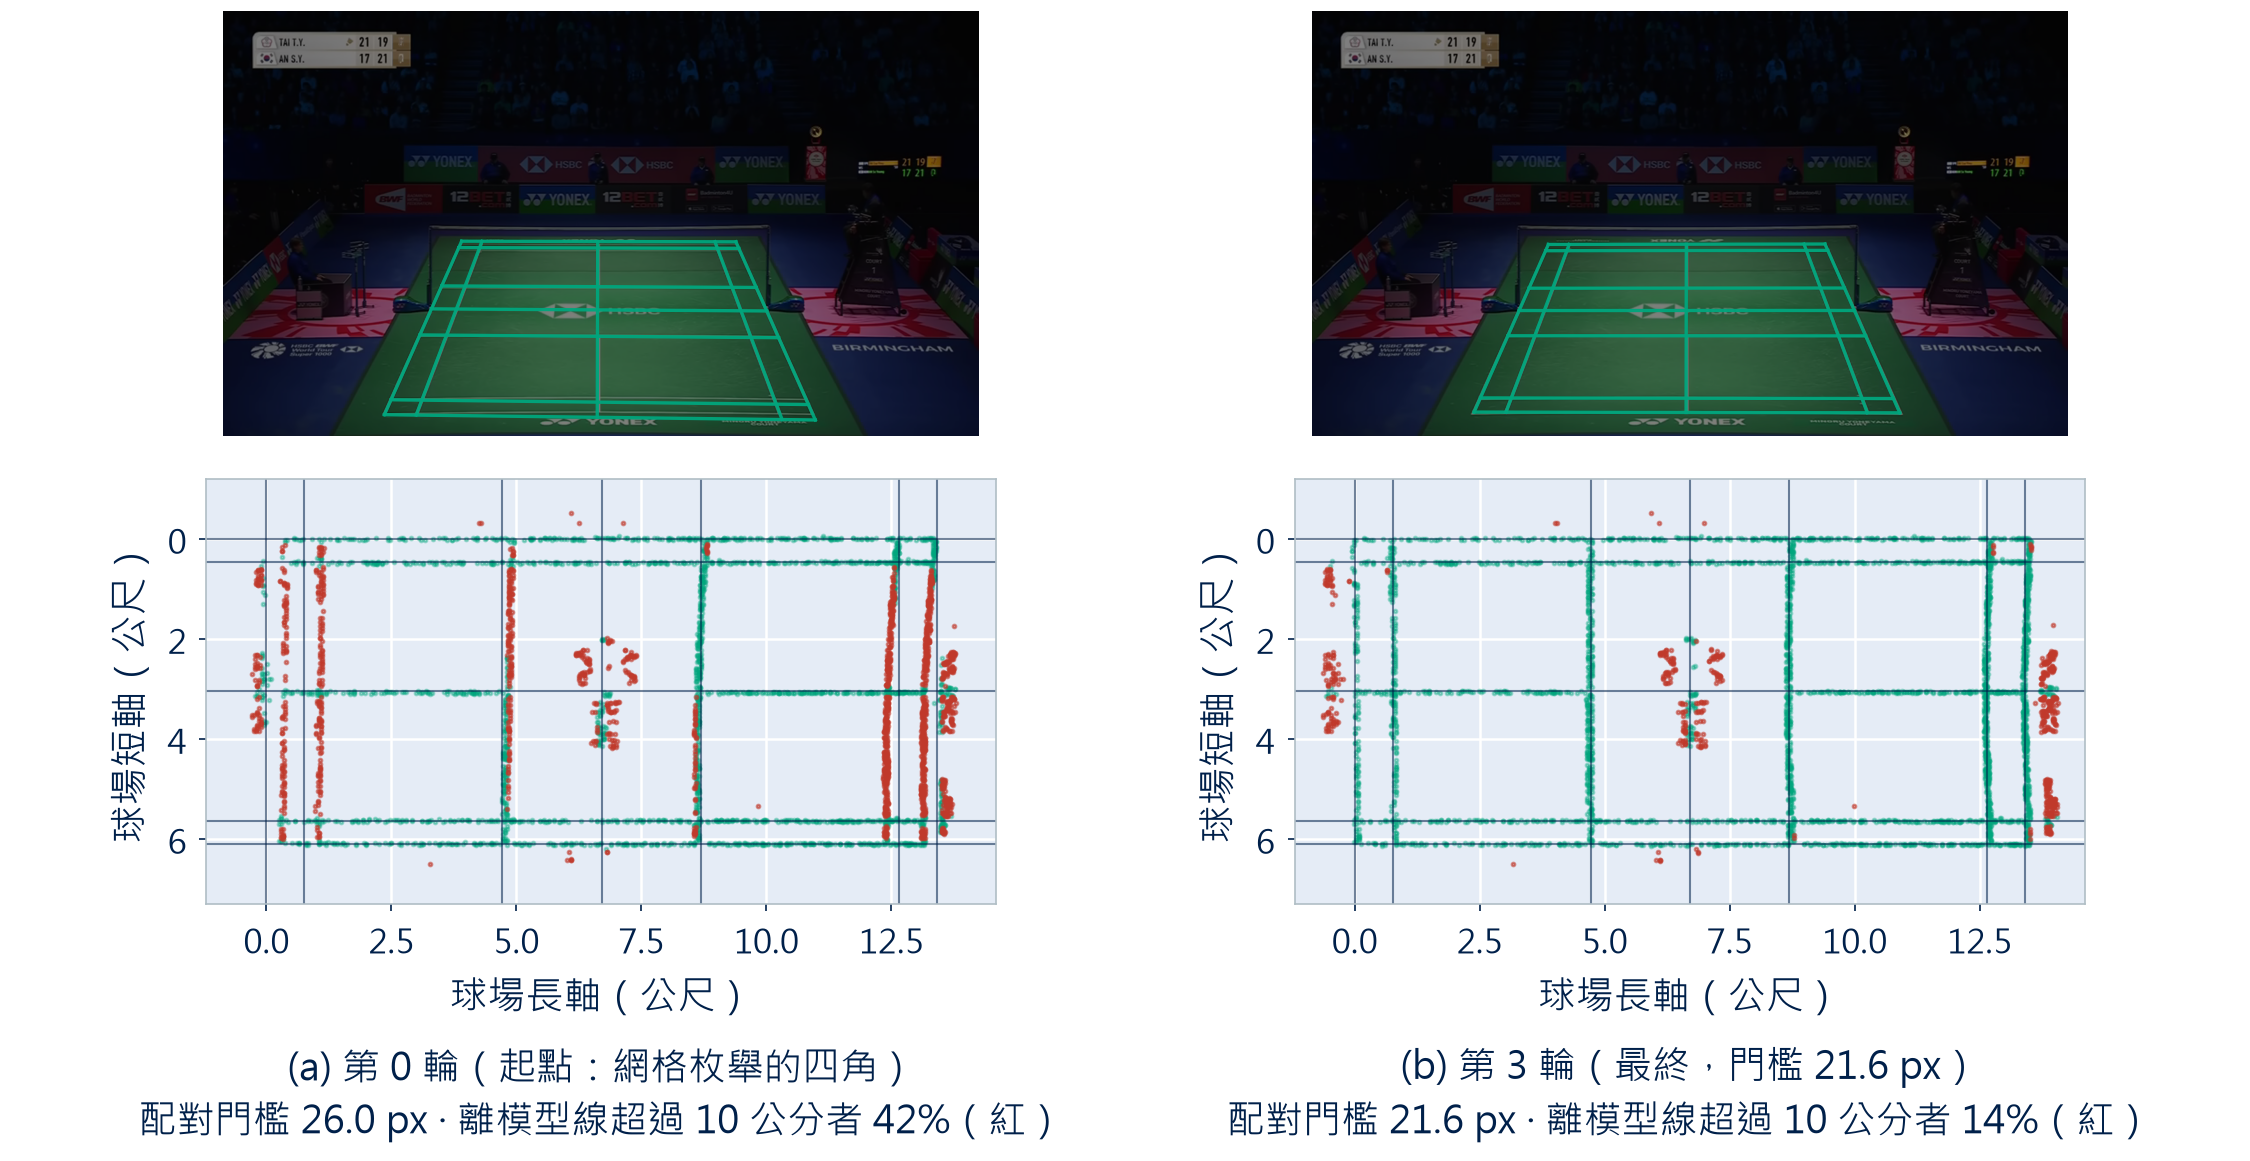
\includegraphics[width=\linewidth]{court_detection/icp.png}
  \caption{ICP 第一輪與最終輪的網格與反投影殘差}
  \label{fig:icp}
\end{figure}

\textbf{邊界修正：}透視壓縮下球場遠端的內、外邊界在畫面上靠得很近，全域解無從分辨，外邊界可能整條鎖到內側線上。本步驟只動四條外邊界，把某條投影線附近的像素依「離線多遠」投到一維直方圖，每條平行線形成一個峰，二維的找線因此降為一維的找顯著峰（\figref{fig:perp-profile}）。遠端刻意偏取最外側的峰重新擬合邊界，因為兩種誤差不對稱，外邊界略往場外時場內物體的相對位置仍成立、下游影響有限，一旦鎖進內側則截斷場內內容、不可逆。搜尋帶寬由寬到窄逐級縮小。這是帶方向的推測，故結果不直接採用，而是回到吻合度評分重算，只有分數未明顯變差才取代原解（\figref{fig:boundary-refine}）。

\begin{figure}[H]
  \centering
  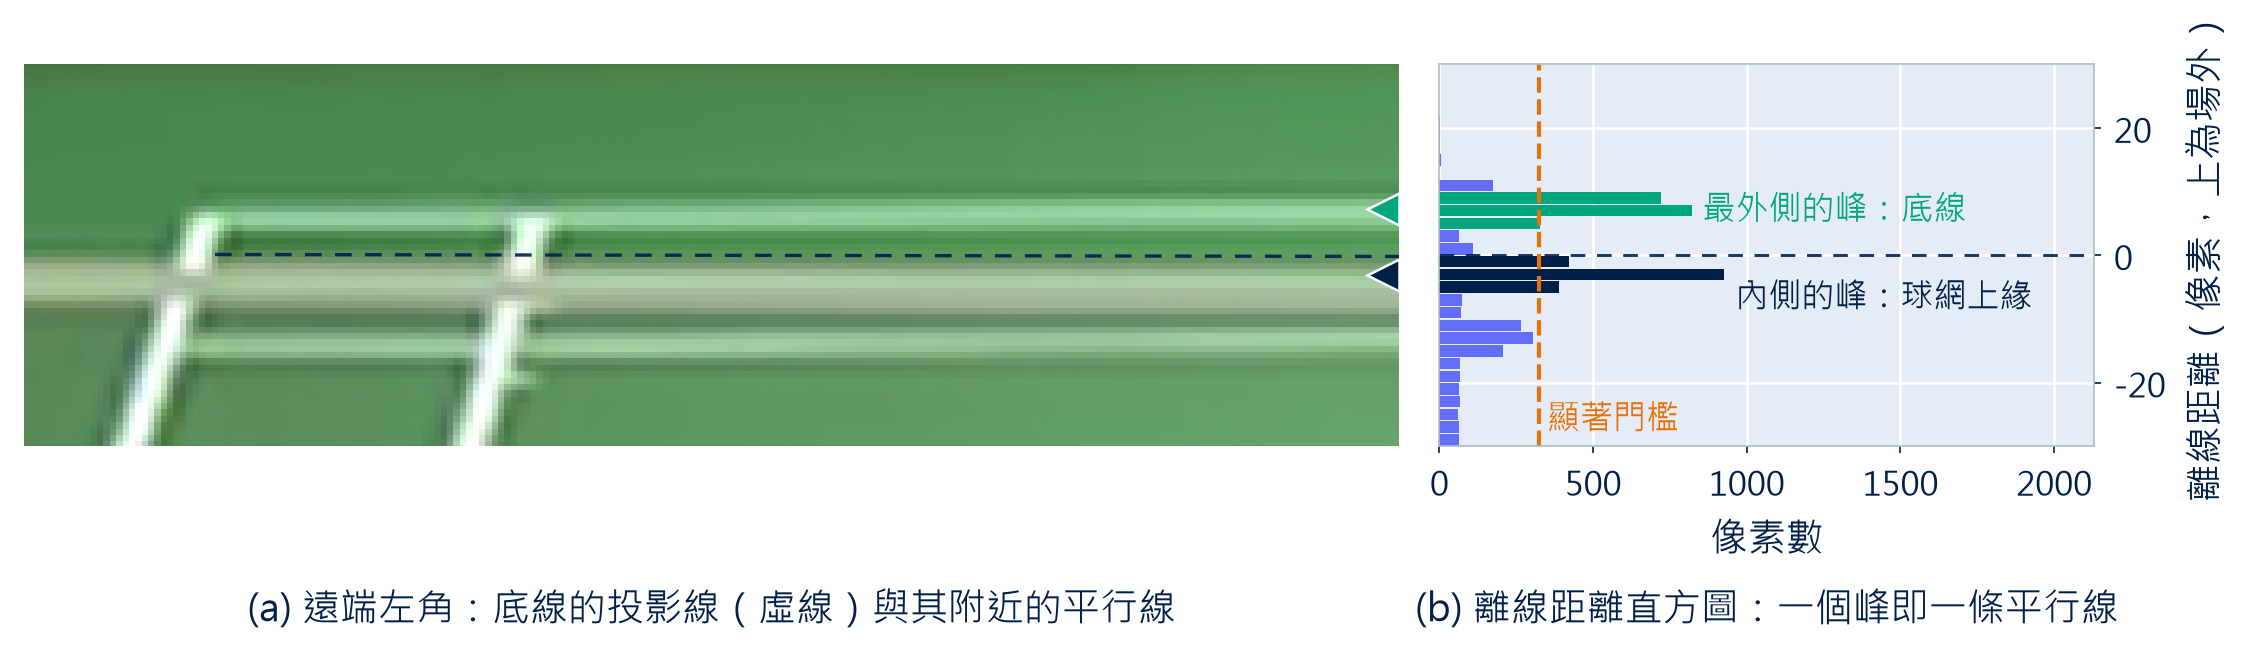
\includegraphics[width=\linewidth]{court_detection/perp_profile.png}
  \caption{投影線的鄰近像素與其離線距離直方圖}
  \label{fig:perp-profile}
\end{figure}

\begin{figure}[H]
  \centering
  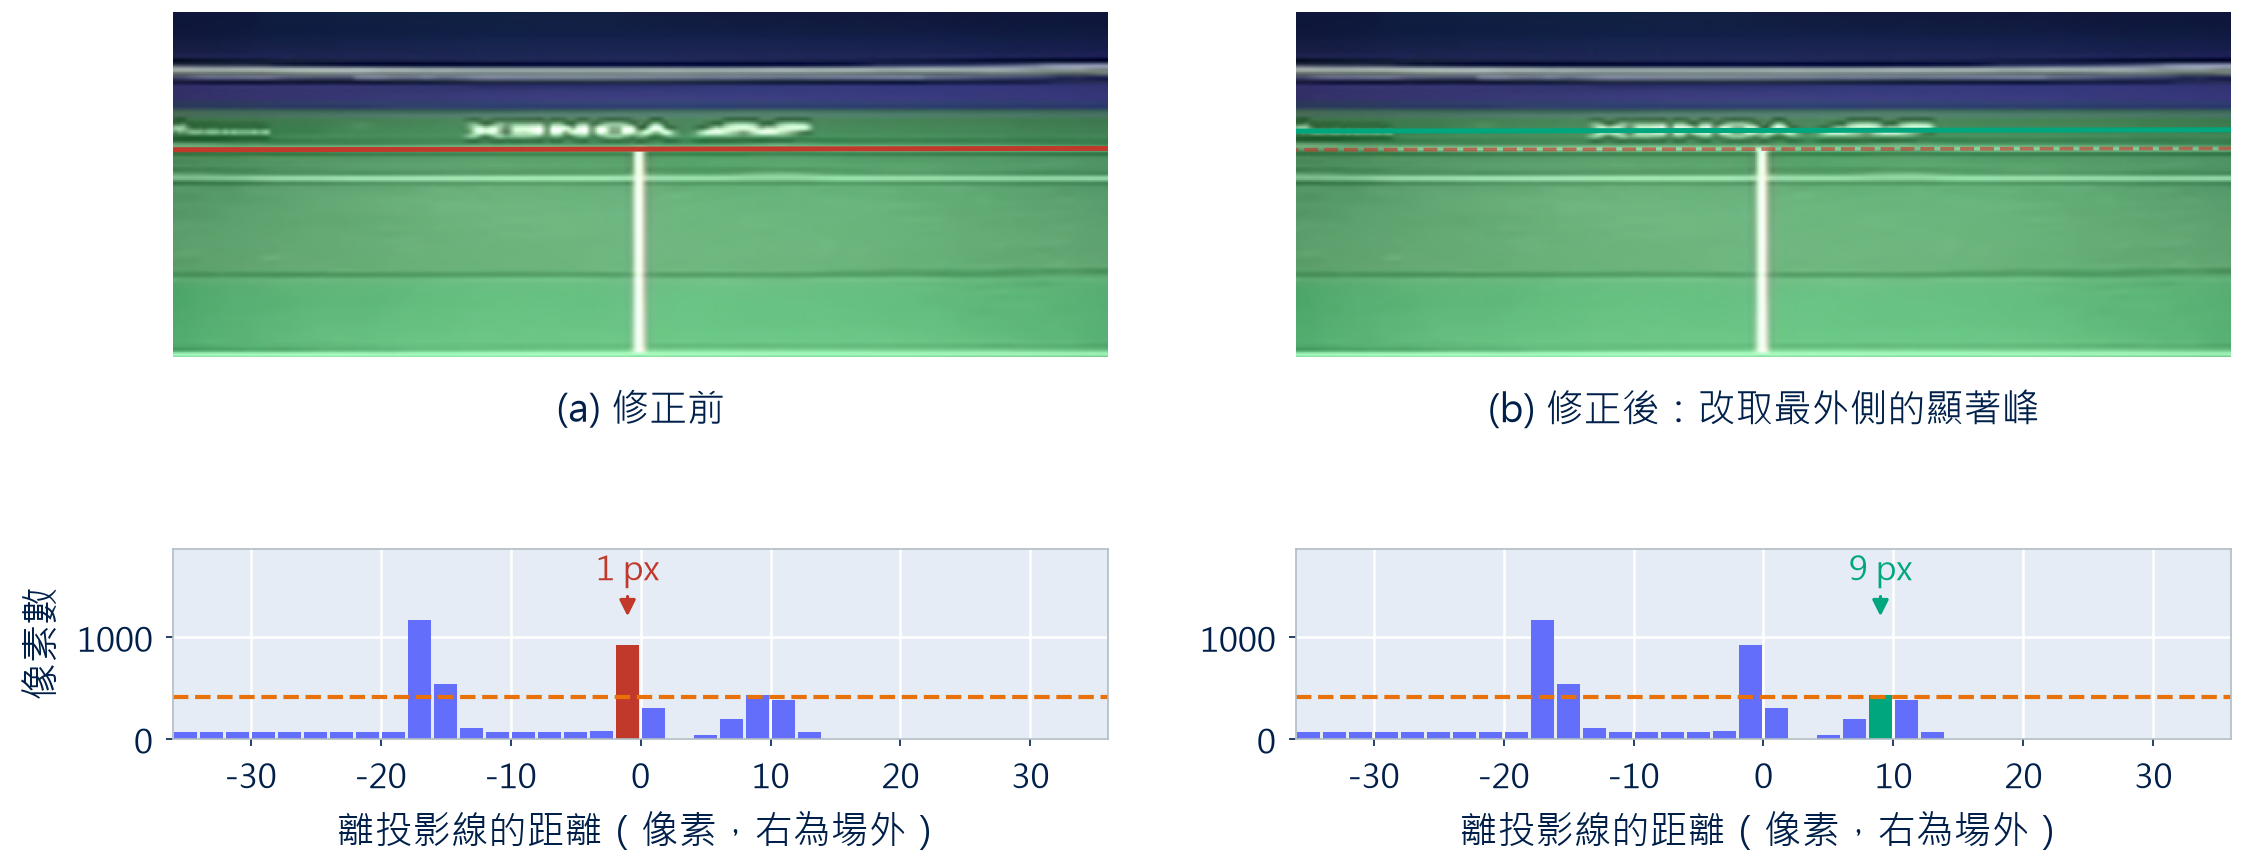
\includegraphics[width=\linewidth]{court_detection/boundary_refine.png}
  \caption{遠端底線由內側峰改取最外側峰的前後對比}
  \label{fig:boundary-refine}
\end{figure}

\subsubsection{結果驗證與評分}

前述步驟以多假設並行：球場區域定位產生二至三組遮罩，場線偵測再對每組遮罩各給三種外角候選，故候選池大小為遮罩組數乘以三，每個候選都帶著它所依據的線像素圖。本步驟把這一池候選收斂成唯一答案，每個候選經角點重估與邊界修正後，在自己的線像素圖上算出吻合度評分，全部比較之下取最高者，其四角與單應性即為模組的最終輸出（\figref{fig:eval-pool}）。

\begin{figure}[H]
  \centering
  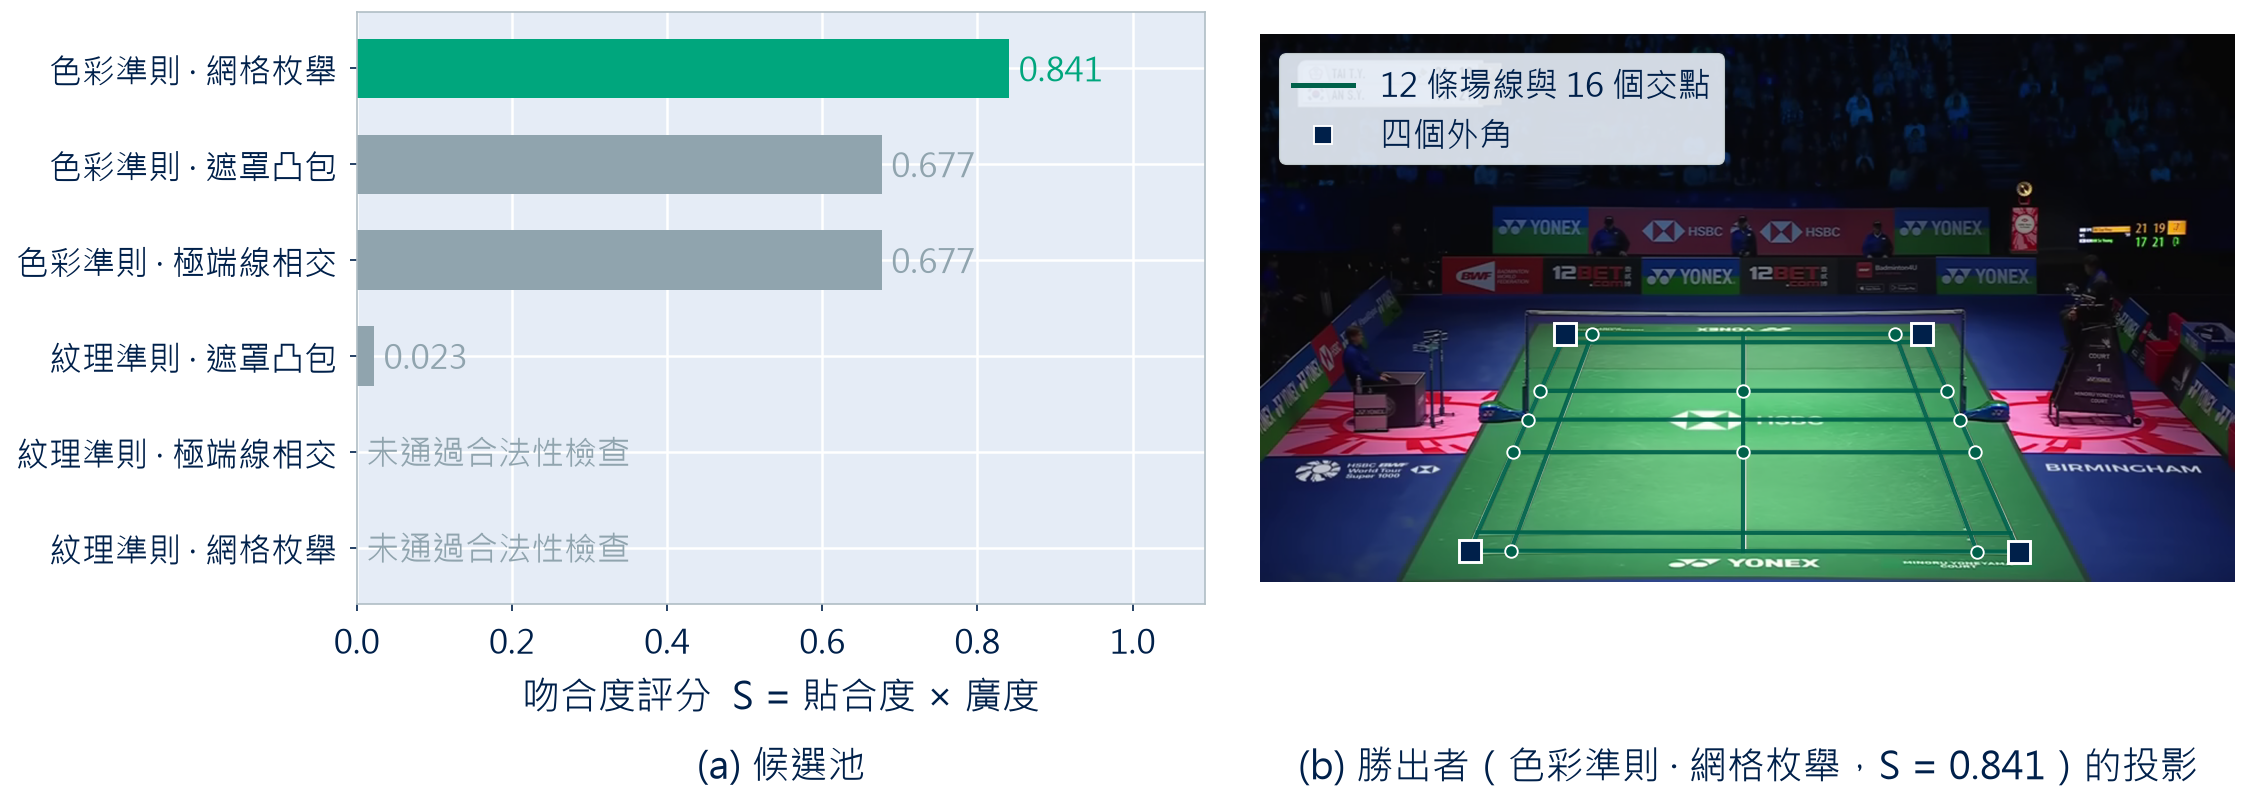
\includegraphics[width=\linewidth]{court_detection/eval_pool.png}
  \caption{候選池的吻合度評分與勝出者的投影}
  \label{fig:eval-pool}
\end{figure}

\subsection{球員骨架追蹤}
\label{sec:pose-tracking}

\subsubsection{概述}

\textbf{問題與目標：}球種分類需要球員的肢體姿態，本模組為每個片段還原場上兩名球員逐幀的骨架，作為下游球種分類的輸入。難點一是廣角轉播下球員在畫面裡常只有一兩百像素高，手肘、手腕等末端關節不易估準。難點二是畫面中除兩名球員外還有裁判、線審、球僮與觀眾，每個人都有骨架可抽，必須靠球場幾何從中認出真正的球員。

\textbf{設計重點：}本模組的核心不在姿態模型本身，而在如何從畫面中的眾多人體骨架穩定選出真正上場的兩名球員。利用球場幾何與跨幀行為自適應完成，主要有兩點做法：

\begin{enumerate}
  \item \textbf{球場座標選人：}系統把每個候選人的腳點反投影到正規化球場座標，依所在半場判定遠、近端身分，再綜合場內位置與透視校正後的身高挑選球員。
  \item \textbf{長短期時序資訊：}系統先從整場候選人的落點分布找出長時間不動的裁判、線審等靜態錨點並排除，再以短期位置記憶維持同一球員的連續身分。
\end{enumerate}

\textbf{處理流程總覽：}如\figref{fig:pose-tracking-flow}。

\begin{figure}[H]
  \centering
  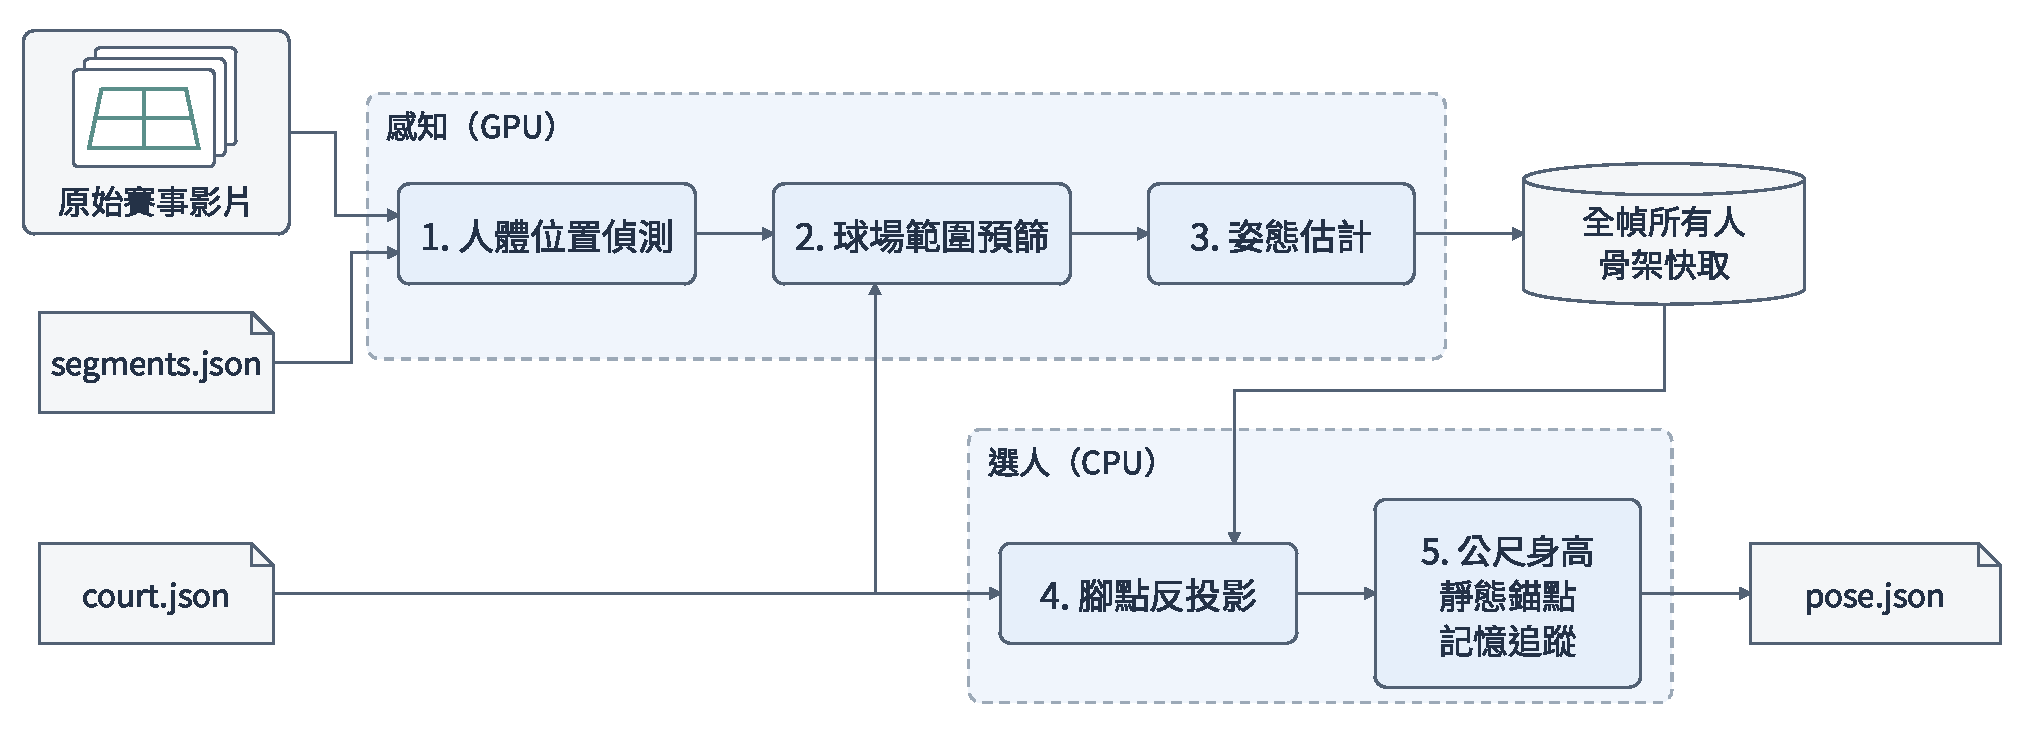
\includegraphics[scale=\flowscale]{pose-tracking.pdf}
  \caption{球員骨架追蹤處理流程}
  \label{fig:pose-tracking-flow}
\end{figure}

\subsubsection{感知：人體偵測與姿態估計}

第一階段為片段的每一幀還原畫面上所有人的骨架並快取，是整個模組的 GPU 時間瓶頸。先用人體偵測器（YOLOX）框出所有人，再採由上而下路線逐人裁切、放大回模型輸入尺寸後在滿解析度下估骨架（RTMPose），讓很小的球員仍能得到準確的關節點（\figref{fig:top-down}）。由於逐人估骨架的成本隨人數線性成長，而每幀偵到的十幾二十人裡真正相關的只有兩到四人，估骨架前先借單應性把每個人的腳點反投影回球場座標，只讓落在放寬球場範圍內者進入姿態模型。

\begin{figure}[H]
  \centering
  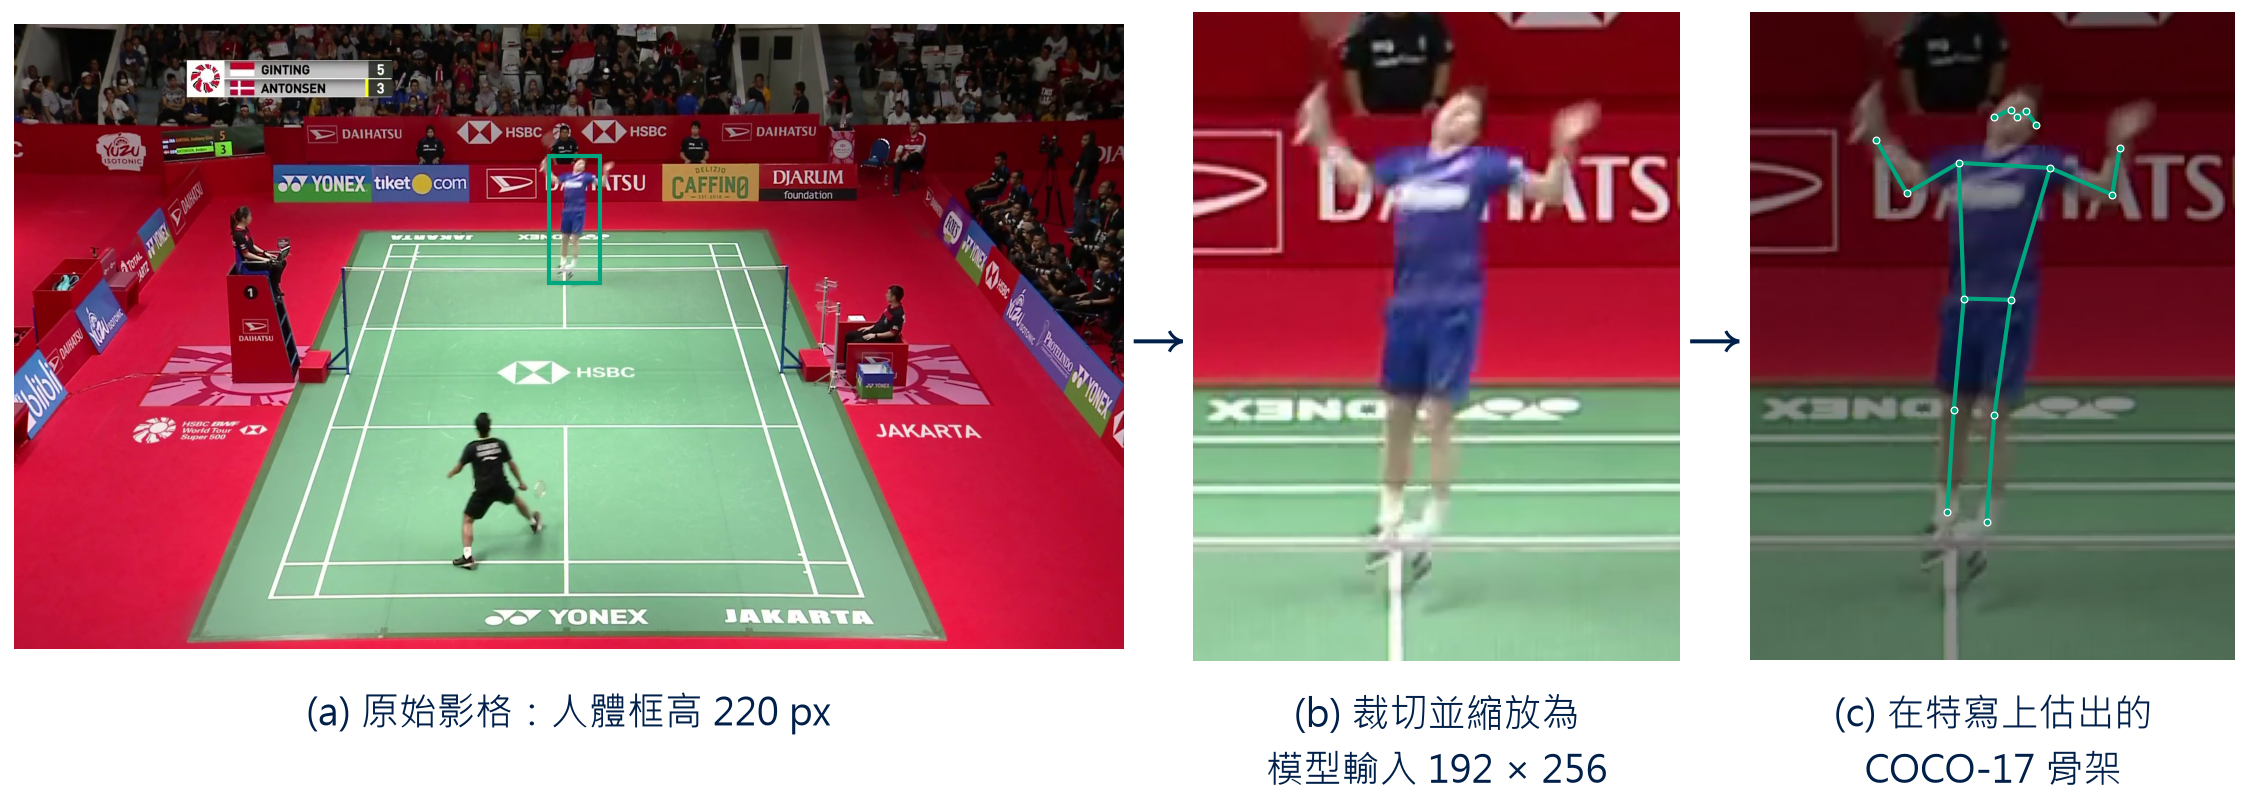
\includegraphics[width=\linewidth]{pose/top_down.png}
  \caption{由上而下，先裁切放大再估骨架}
  \label{fig:top-down}
\end{figure}

\subsubsection{選人：腳點與球網分半}

第二階段在快取好的骨架上以純幾何認出 \texttt{top}、\texttt{bottom} 兩名球員。把每個人化約為一個雙踝中點，經單應性反投影落到正規化球場座標。每一半內通過球場邊界的候選人可能不只一個，因此需要以下的排名與排除準則挑出球員。

\textbf{公尺身高排名：}不能直接選最高的人，像素高度會被透視扭曲。因此先借單應性量出畫面上每點「一公尺對應多少像素」，把候選人放到同一真實尺度上比身高。

\textbf{非對稱邊界放寬：}單應性只在地平面上成立，球員起跳殺球時腳踝離地，反投影會把腳點推到底線之外。為此把場內範圍在底線方向（縱向）放寬、邊線方向（橫向）收緊（\figref{fig:court-select}）。

\begin{figure}[H]
  \centering
  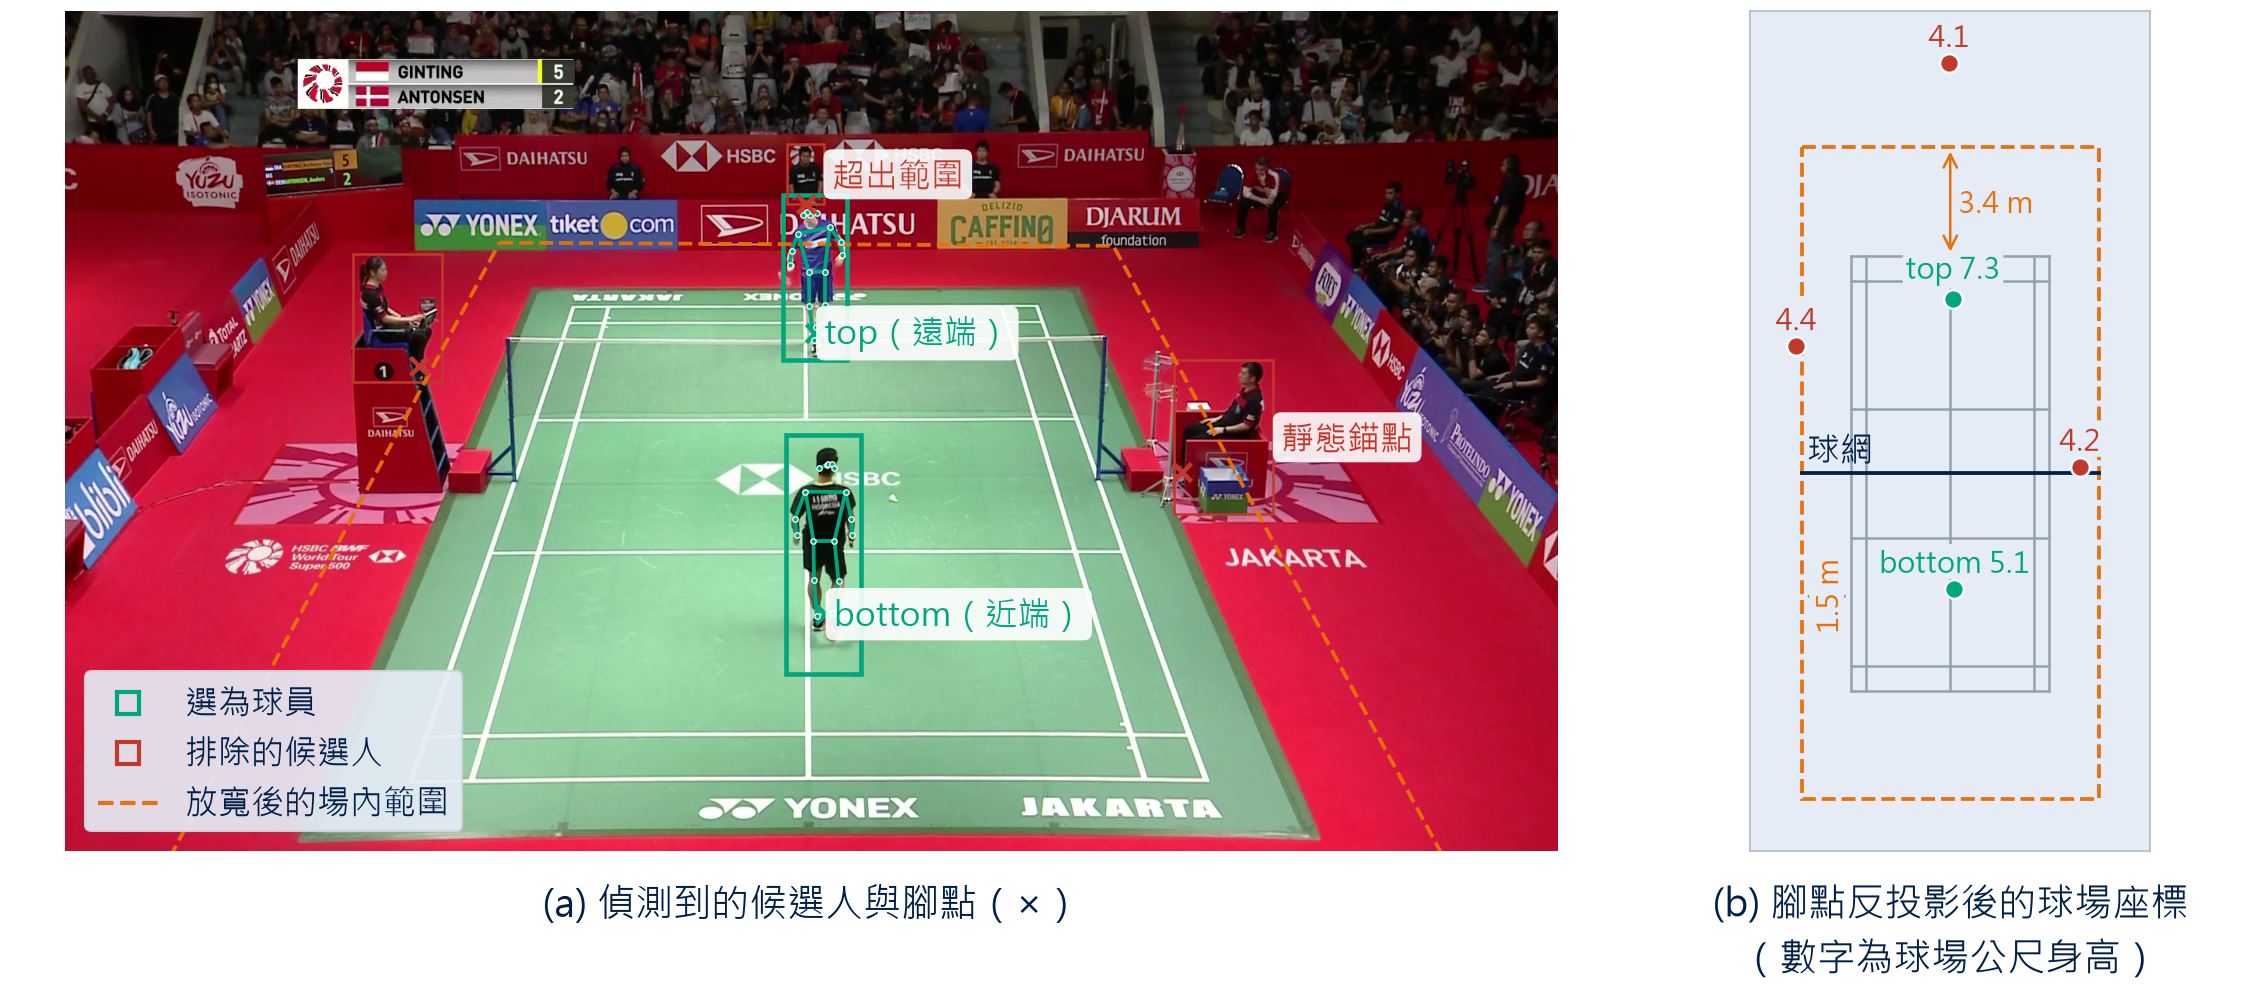
\includegraphics[width=\linewidth]{pose/court_select.png}
  \caption{腳點反投影至球場座標}
  \label{fig:court-select}
\end{figure}

\textbf{靜態錨點排除干擾：}尺寸與邊界仍擋不住一種情形，站在底線後、身高又與遠端球員相當的裁判，一旦真球員該幀被漏偵便可能頂替上來。關鍵在於是否移動，官員整場腳點落在同一處，球員則掃過整個球場。統計整場每個候選人的腳點落點，把在很高比例的幀裡被占用且幾乎不動的格子標為靜態錨點，之後腳點離錨點太近的候選人一律拒絕（\figref{fig:static-anchors}）。

\begin{figure}[H]
  \centering
  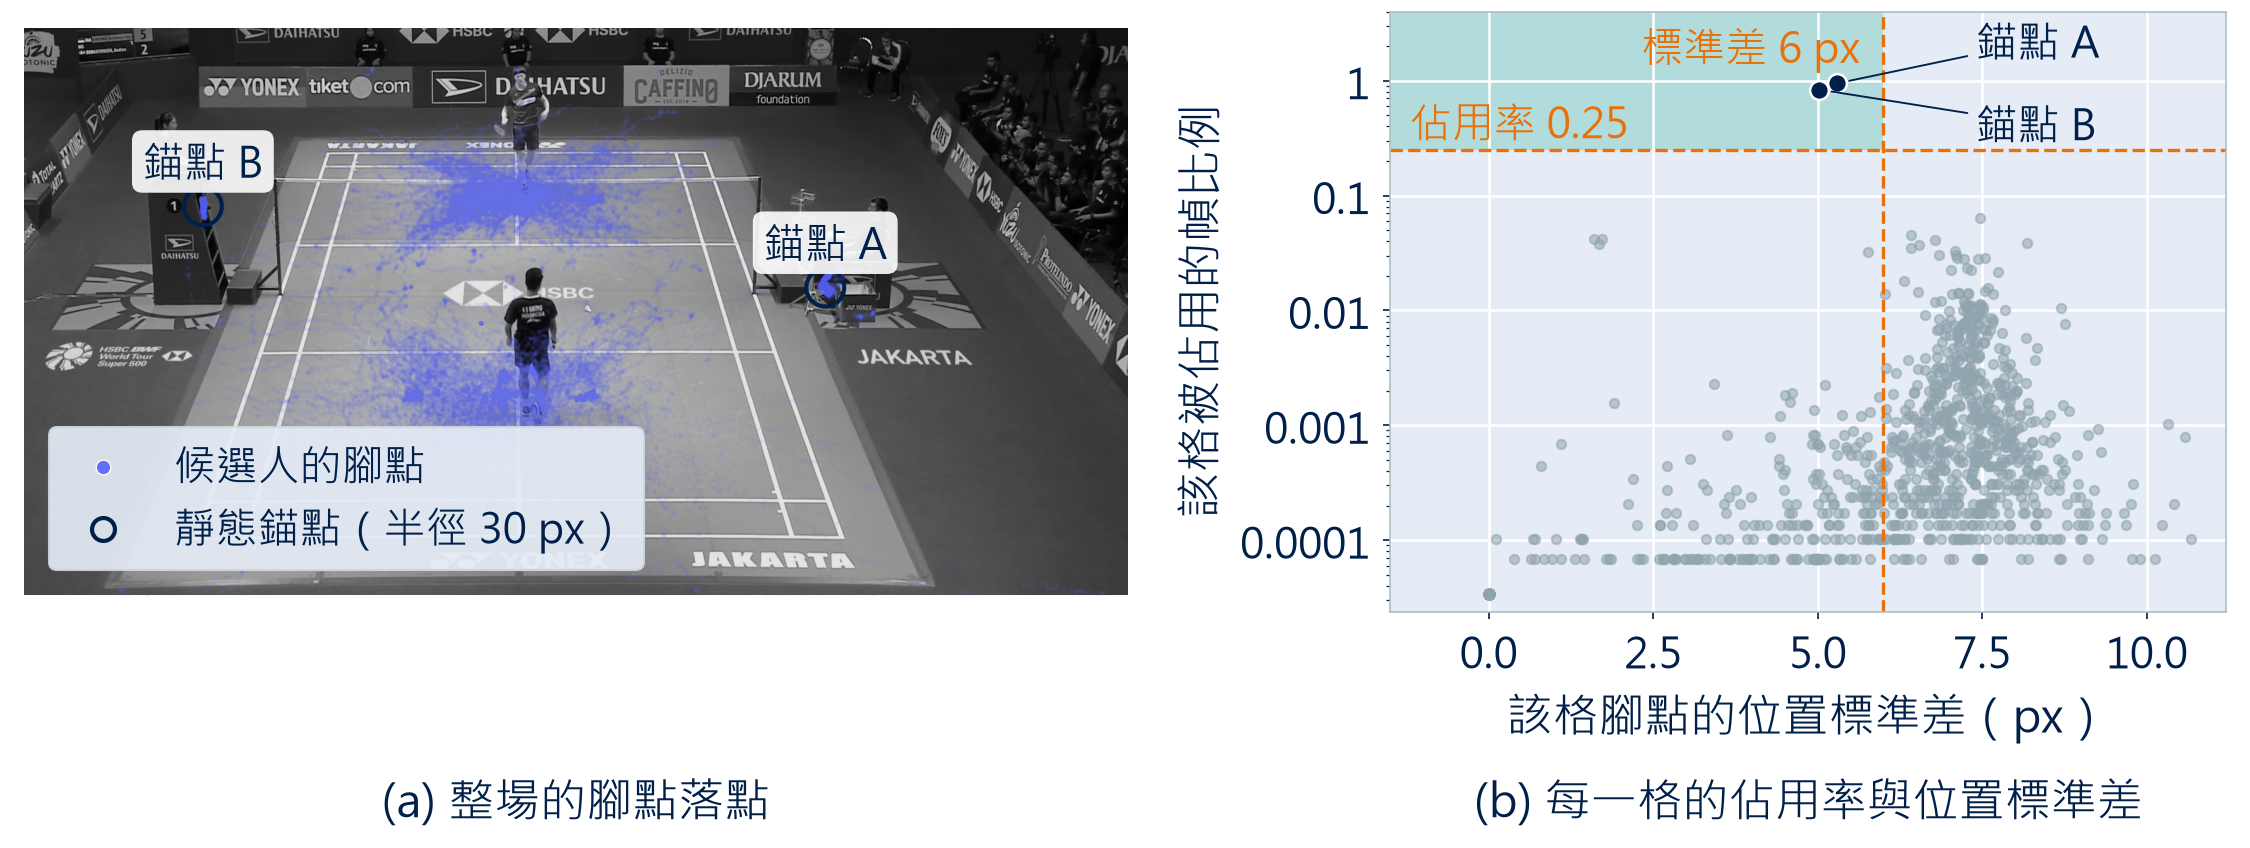
\includegraphics[width=\linewidth]{pose/static_anchors.png}
  \caption{整場腳點落點，固定不動者被判為靜態錨點}
  \label{fig:static-anchors}
\end{figure}

\textbf{有記憶的連續追蹤：}逐幀獨立選人仍會偶爾跳錯人，故改用帶短期記憶的追蹤器，有記憶時選離「上一幀所在位置」最近的人。記憶過舊即作廢，下一幀重新起始時無前一位置可依靠，便退回用公尺身高挑最高者。連續性成為依據，把漏偵時誤選裁判的風險壓到最低。

\section{球體分析}
\label{sec:shuttle-analysis}

\subsection{球體追蹤與軌跡重建}
\label{sec:shuttle-tracking}

\subsubsection{概述}

\textbf{問題與目標：}本模組為每個固定機位比賽片段重建羽球在畫面中的逐幀位置，作為下游擊球時刻偵測與球種分類的基礎。難點在於目標小、速度快，且球常被球員、球拍與球網遮擋。

\textbf{設計重點：}本模組沿用預訓練的 TrackNetV3，並利用時間連續性與運動約束，改善單幀偵測的誤判與缺失，主要有兩點做法：

\begin{enumerate}
  \item \textbf{多候選軌跡搜尋：}以低門檻保留每幀多個候選，再用 Viterbi 找出整段最連貫的路徑，使微弱但連續的真球能排除高信心的孤立誤偵。
  \item \textbf{互補雙軌跡：}同時輸出覆蓋率較高的 InpaintNet 軌跡與較保守的 Viterbi 軌跡，供下游依任務分工使用。
\end{enumerate}

\textbf{處理流程總覽：}如\figref{fig:shuttle-tracking-flow}。

\begin{figure}[H]
  \centering
  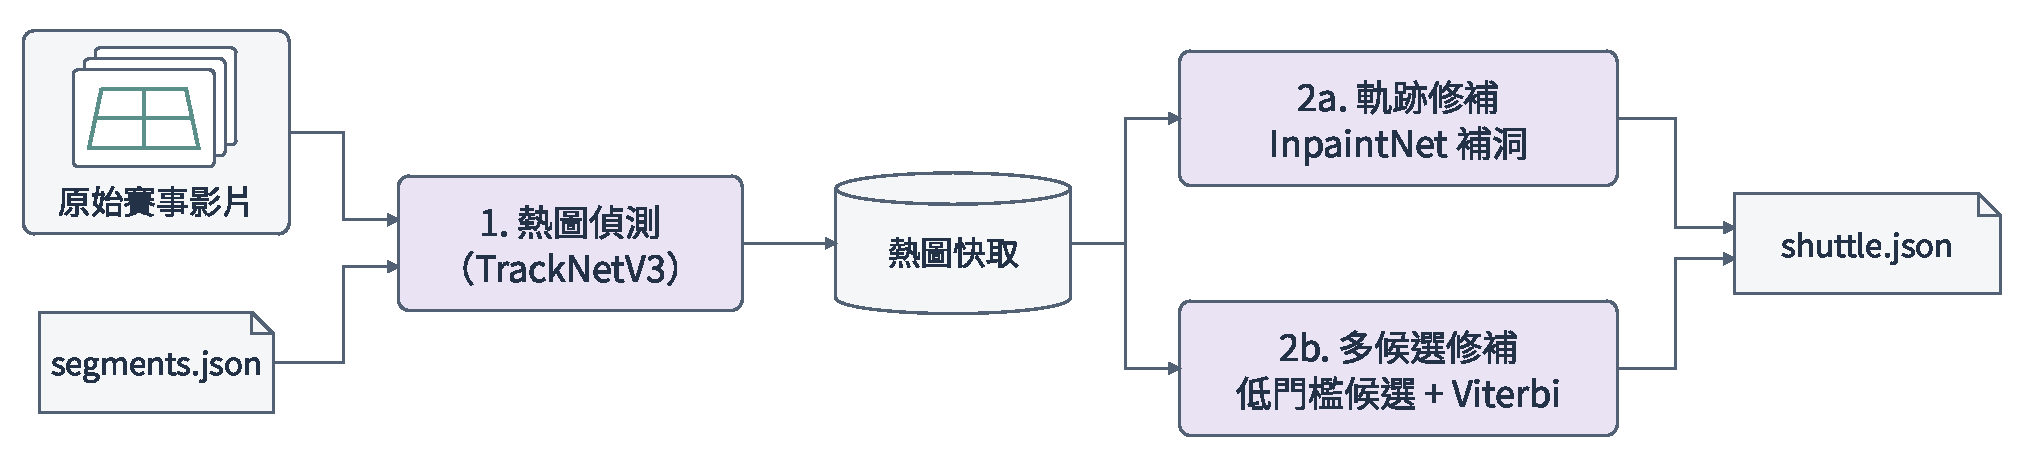
\includegraphics[scale=\flowscale]{shuttle-tracking.pdf}
  \caption{球體追蹤與軌跡重建處理流程}
  \label{fig:shuttle-tracking-flow}
\end{figure}

\subsubsection{熱圖偵測與快取}

第一階段要在極小又易與背景混淆的目標上給出可靠證據。系統使用 TrackNetV3 對連續影格進行推論，產生逐幀信心熱圖。熱圖能保留多個可能位置，使後續方法可利用時間連續性決定最合理的軌跡。由於熱圖推論是主要的 GPU 運算，系統將結果按片段快取，使 InpaintNet 與 Viterbi 能共用相同的偵測結果，並可在不重新推論的情況下反覆調整軌跡重建方法。

先以 largest-blob 讀出一條基準軌跡，用信心門檻二值化後取面積最大的連通區塊，以其中心為位置、區塊峰值為該幀信心（\figref{fig:heatmap-readout}）。這條基準軌跡是修補法的輸入，而選擇法另從同一份熱圖以低門檻自取候選。

\begin{figure}[H]
  \centering
  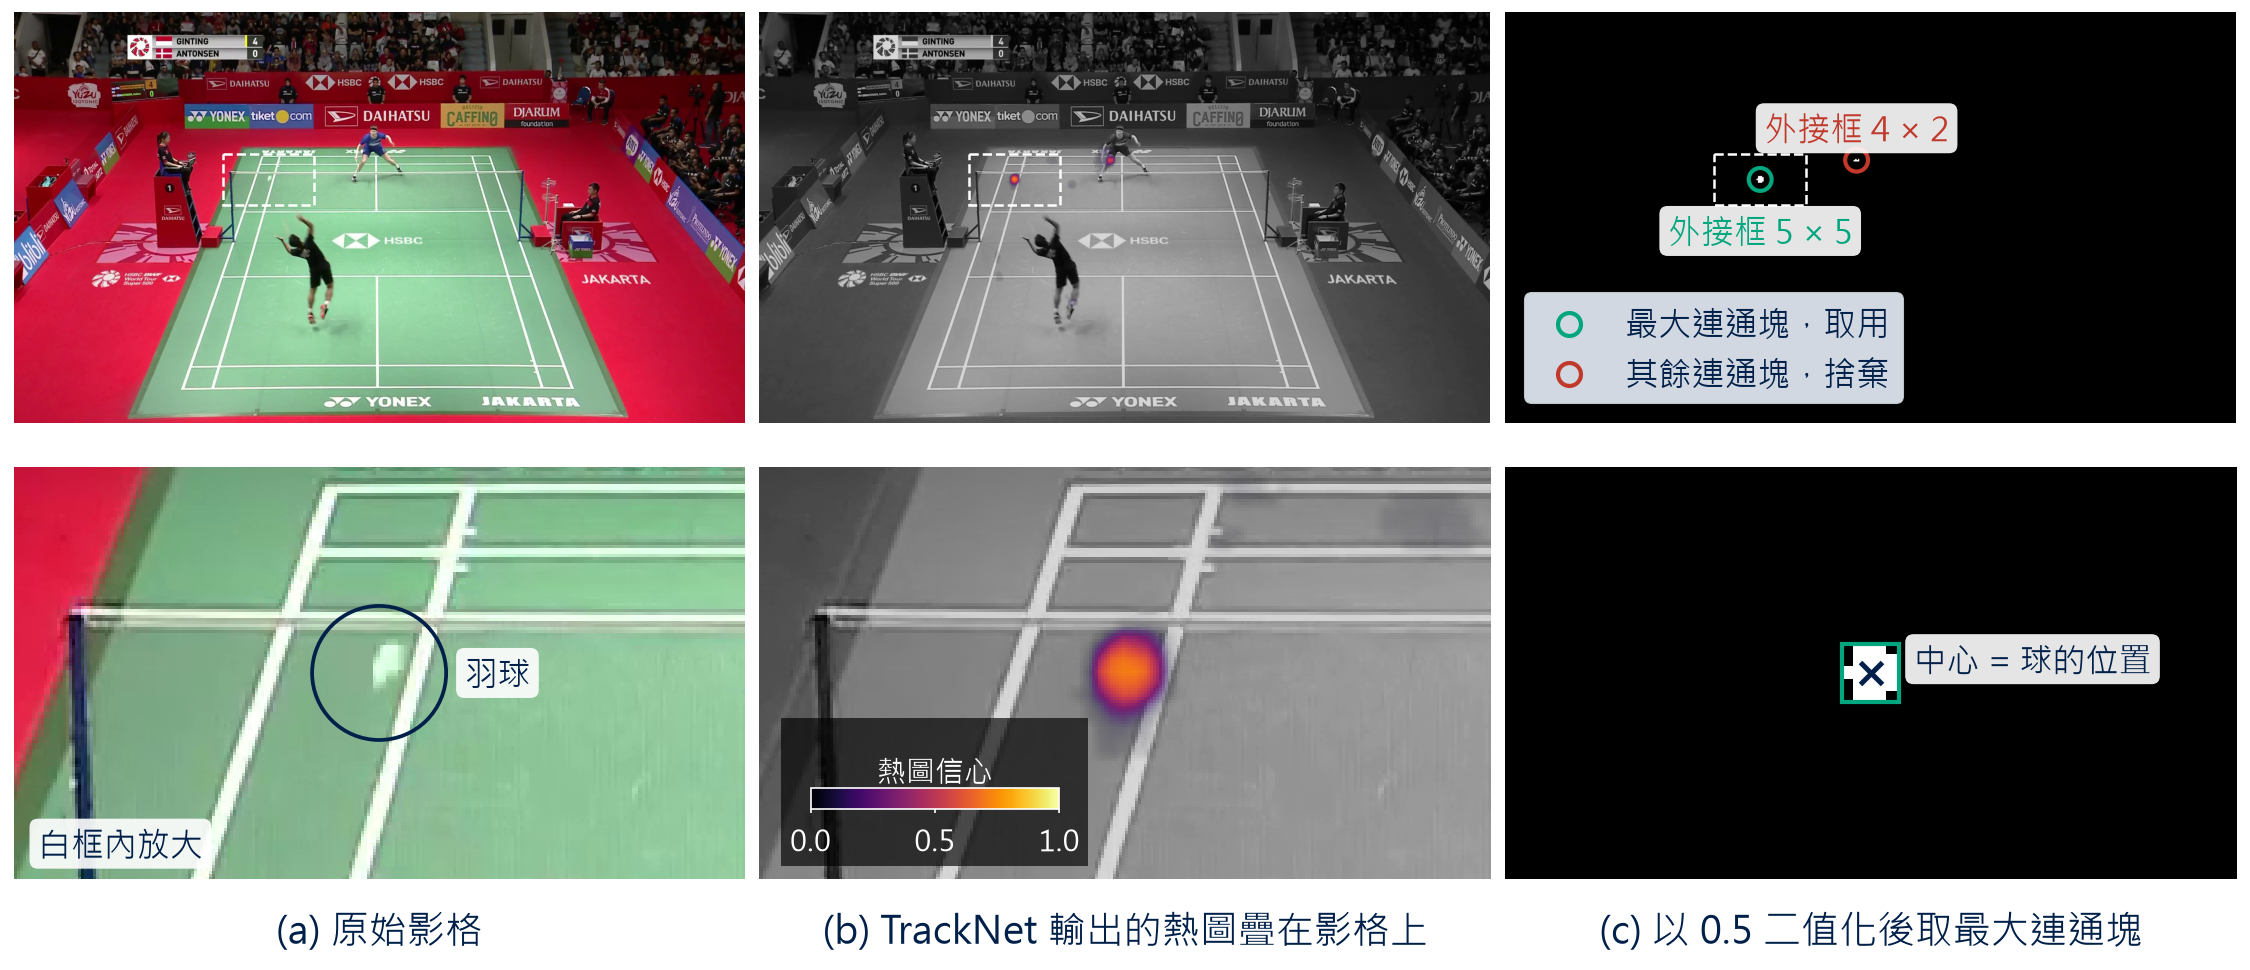
\includegraphics[width=\linewidth]{shuttle_tracking/heatmap_readout.png}
  \caption{從熱圖以 largest-blob 讀出基準軌跡}
  \label{fig:heatmap-readout}
\end{figure}

\subsubsection{軌跡修補（InpaintNet）}

第一種方法先將熱圖二值化，取每幀面積最大的連通區塊作為基準位置，再由補洞網路（InpaintNet~\cite{tracknetv3}）補回遮擋造成的缺幀（\figref{fig:inpaint-gaps}）。補值點的信心標為 0，使下游能區分實際偵測與模型推論。

\begin{figure}[H]
  \centering
  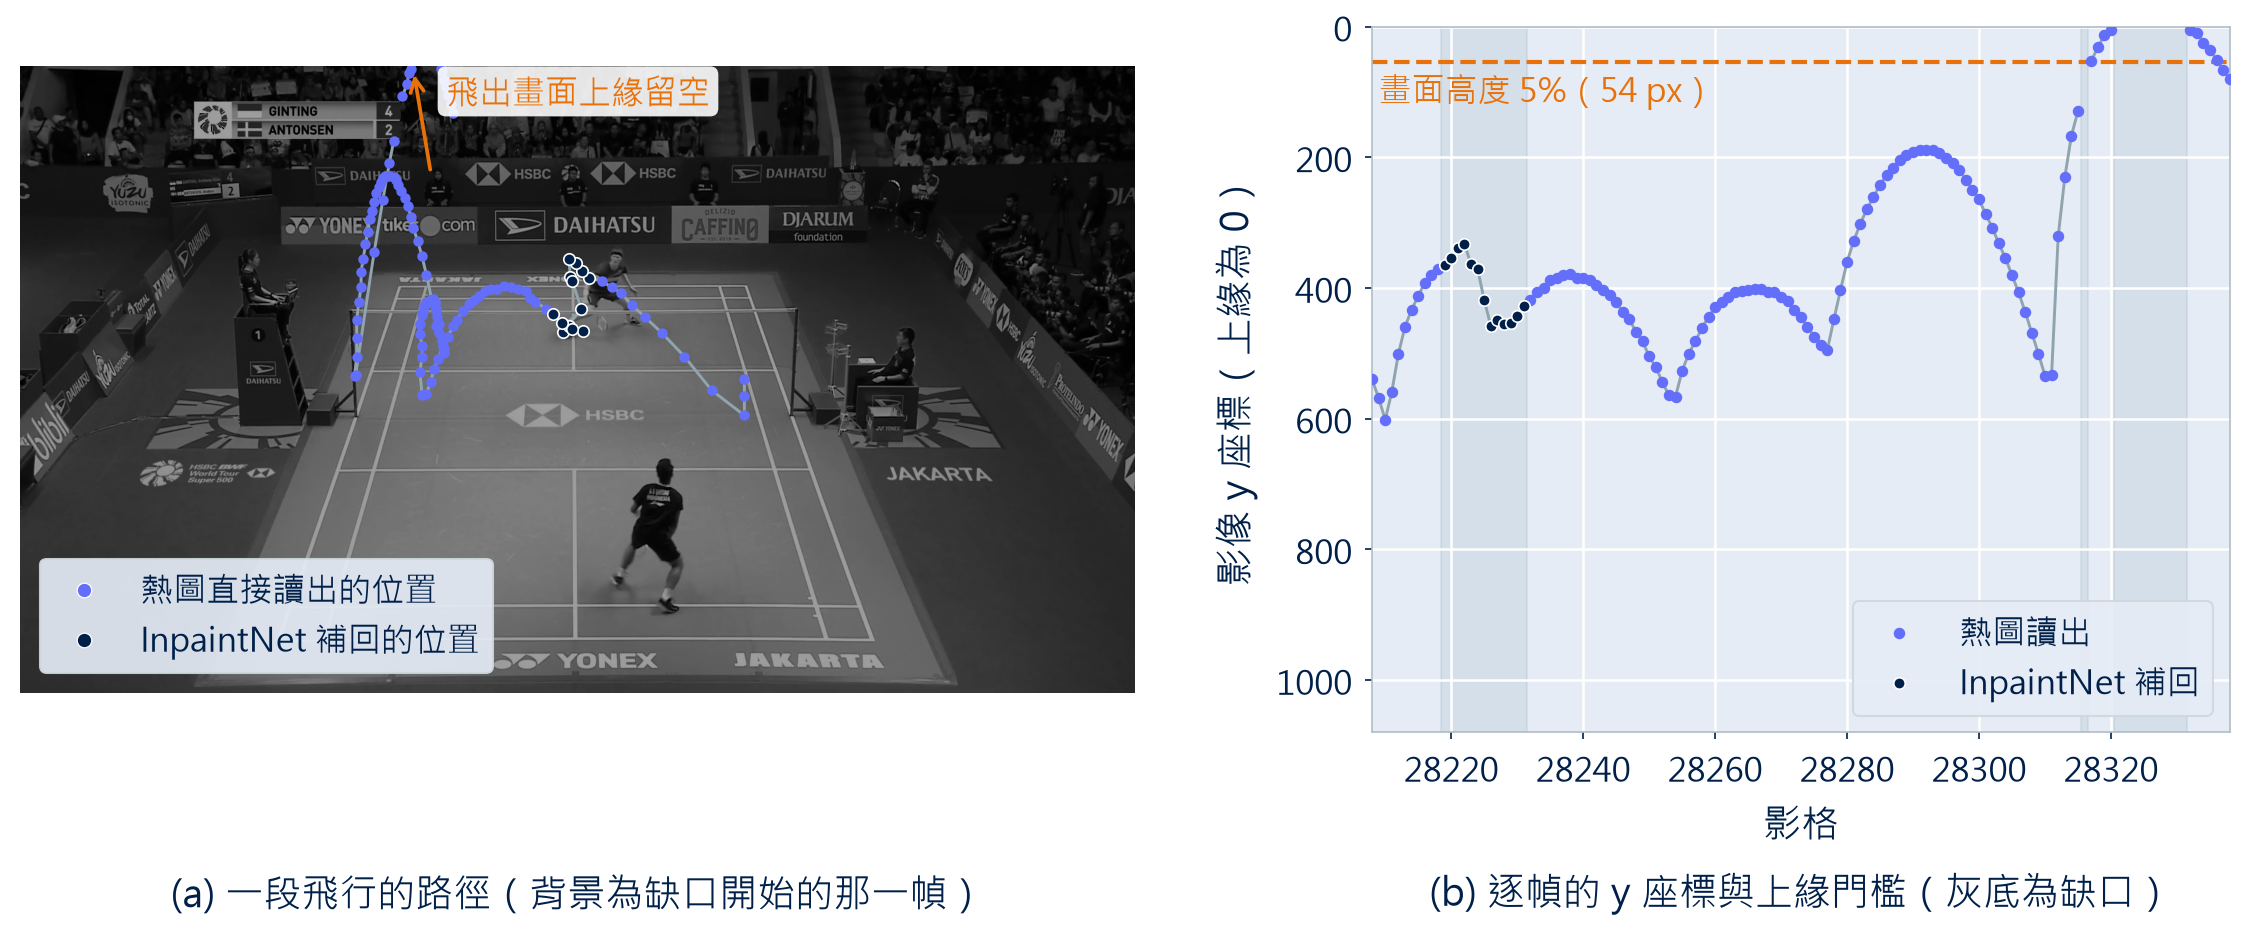
\includegraphics[width=\linewidth]{shuttle_tracking/inpaint_gaps.png}
  \caption{InpaintNet 補回球員遮擋造成的缺幀}
  \label{fig:inpaint-gaps}
\end{figure}

\subsubsection{多候選軌跡修補（Viterbi）}

第二種方法改以全域路徑搜尋壓制孤立誤偵。它用極低門檻把每幀所有稍可能是球的區塊全留作候選，再找一條最像真實飛行的路徑穿過它們。把每幀候選當節點、相鄰候選間連邊，給節點獎勵（信心越高越好）、給邊代價（前後兩點推出的速度越不合物理越貴、跨幀越多越貴），以動態規劃取總分最高的路徑。如此微弱但連貫的偵測能勝過強烈但孤立的偵測（\figref{fig:viterbi-path}）。當某幀球員鞋子或場線在信心上壓過真球，只要接不上前後飛行就不會入選。最後才對剩餘缺口依長度與兩端運動狀態決定補或不補，並以卡爾曼濾波填值。

\begin{figure}[H]
  \centering
  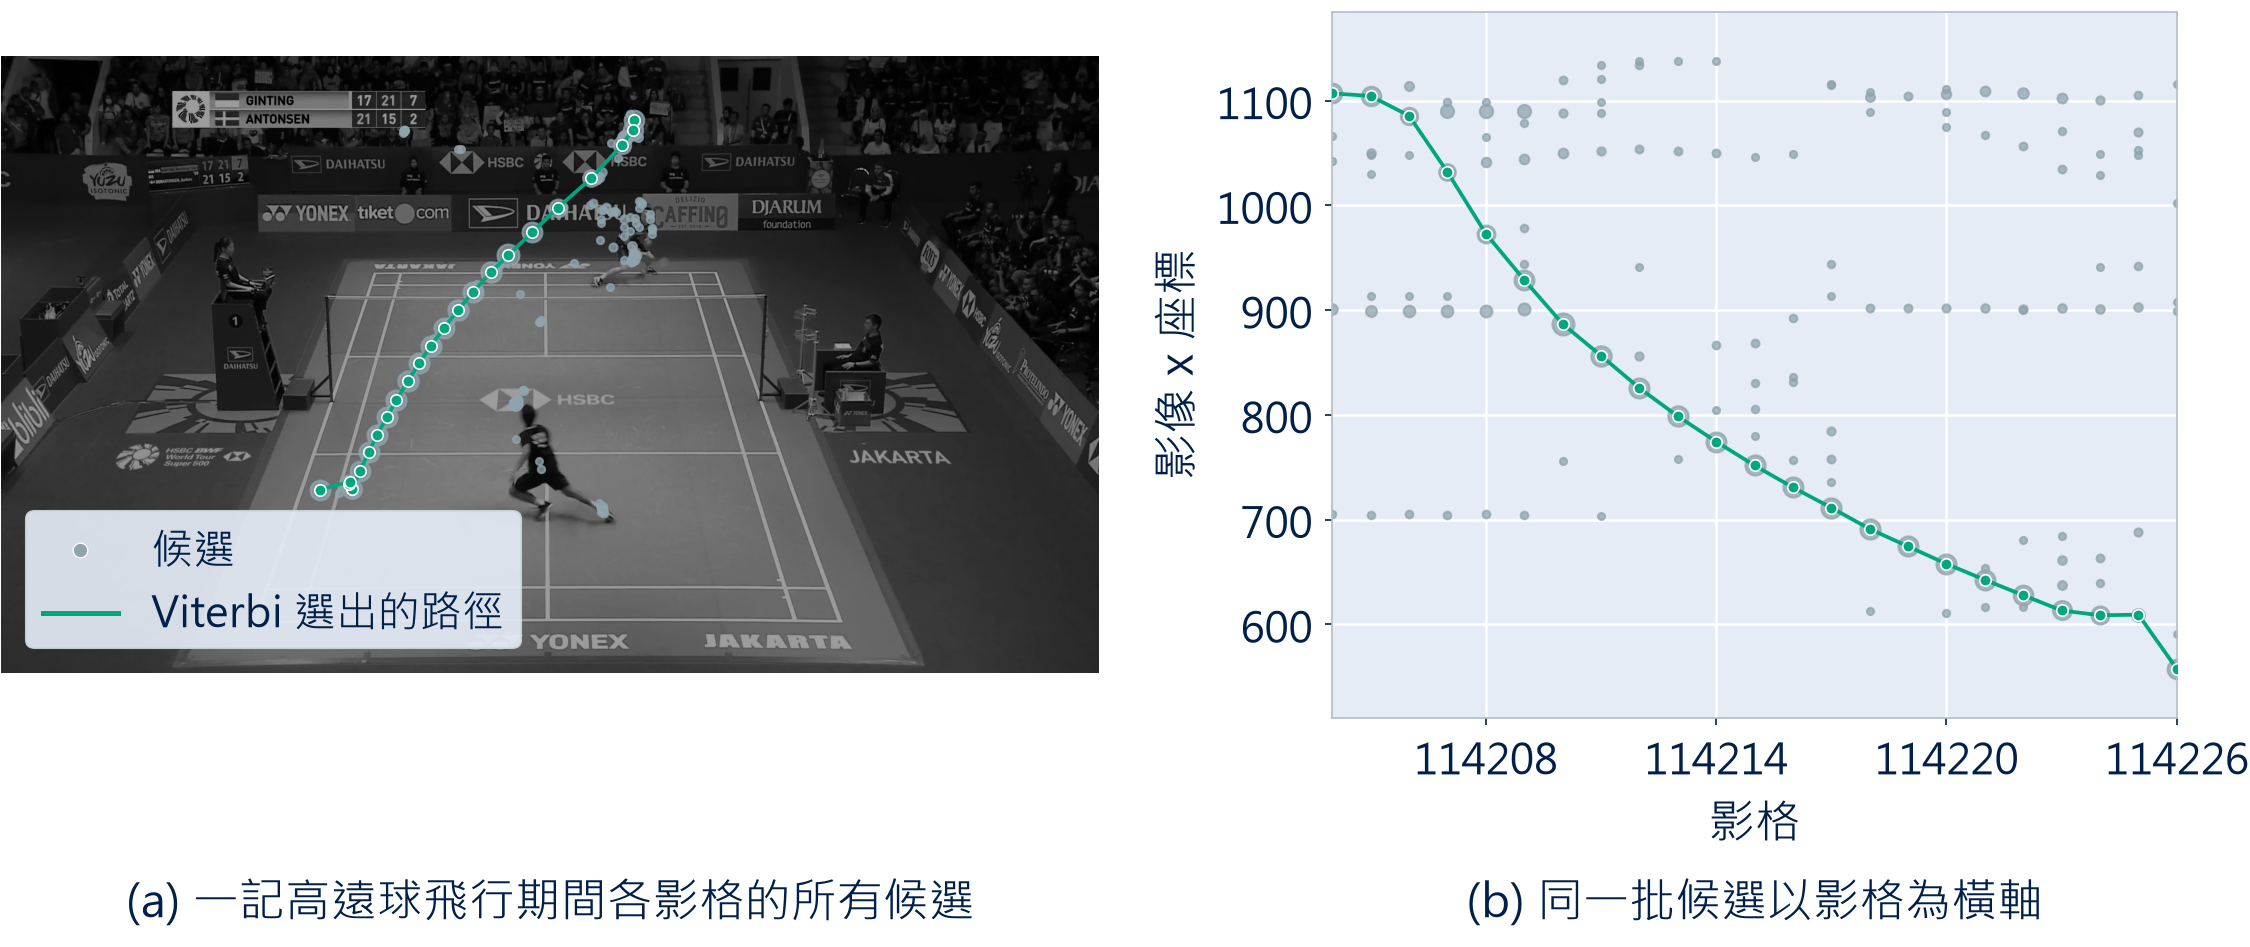
\includegraphics[width=\linewidth]{shuttle_tracking/viterbi_path.png}
  \caption{低門檻多候選與 Viterbi 選出的最佳路徑}
  \label{fig:viterbi-path}
\end{figure}

\subsubsection{雙軌跡並存}

修補法與選擇法各有所長、在不同情境下互有勝負，模組因此不在內部挑出贏家，而是把兩條軌跡都算出、都寫進 \texttt{shuttle.json}，把選擇交給握有更多上下文的下游。

\subsection{擊球時刻偵測}
\label{sec:hit-detection}

\subsubsection{概述}

\textbf{問題與目標：}本模組在每個片段內標記出每一擊球的影格，為下游球種分類提供窗口範圍。

\textbf{設計重點：}本模組的初始版本參考了開源專案 SoloShuttlePose 的擊球事件偵測（\texttt{event\_detect}）~\cite{soloshuttlepose}，其僅以單條球體軌跡的 Y 軸峰值與軌跡轉角判定擊球。現行版本在其基礎上重新設計，改以多源證據融合與結構性補漏取代單一軌跡幾何。一次擊球是軌跡上一瞬間的事件，只在球路上留下細微痕跡，任何單一訊號都不夠可靠。本模組因此同時融合多種訊號，並以召回優先，把不漏拍作為首要目標。主要有兩點做法：

\begin{enumerate}
  \item \textbf{多源證據融合：}不押注單一訊號，同時利用兩條球體軌跡、球員骨架與逐幀球種模型三種來源。相對於只讀軌跡幾何的做法，任一來源在特定情境失效時仍能由其他來源補上。
  \item \textbf{結構性補洞：}不靠放寬偵測門檻加球，而是從「結構上一定有一拍」的位置（交替違規、模型長時間鎖定、發球遮擋）反推漏拍位置。
\end{enumerate}

在 8 場未參與開發的比賽上，本模組在 $\pm$5 影格容差下召回率 90.90\%、精確率 95.49\%（見\secref{sec:exp-events}）。

\textbf{處理流程總覽：}如\figref{fig:event-detection-flow}。

\begin{figure}[H]
  \centering
  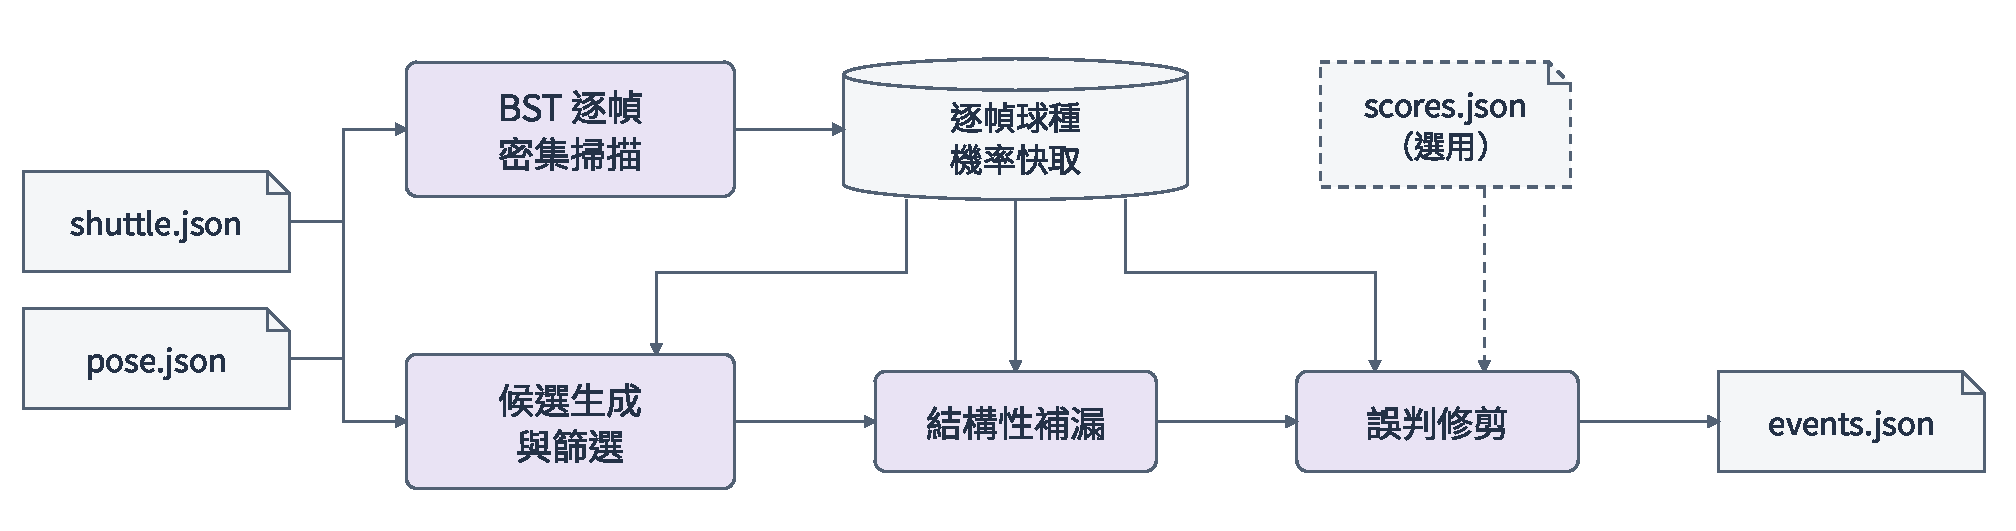
\includegraphics[scale=\flowscale]{event-detection.pdf}
  \caption{擊球時刻偵測處理流程}
  \label{fig:event-detection-flow}
\end{figure}

\subsubsection{逐幀球種證據}

本模組先對每個片段逐影格掃描，將每個影格前後各半秒的窗口，輸入球種分類模型 BST~\cite{bst}，得到該影格的 25 類球種機率分布。

BST 原本設計的窗口是「兩次擊球之間」，需要以擊球時刻作為窗口邊界。但在本模組，擊球時刻正是需要偵測的目標。因此本模組將所有影格以固定窗口輸入模型，並將輸出反過來作為是否存在擊球的判斷依據之一。BST 的輸出提供三種輔助證據（\figref{fig:dense-evidence}）：

\textbf{球種信心：}若模型對某個影格的窗口給出高信心的球種判斷（例如 0.9 的殺球），代表這個窗口的球路與骨架很接近某個真實擊球的樣態。相較於另一個最高信心僅 0.3 的窗口，前者更可能對應到一次真實擊球。

\textbf{擊球者判定：}即使窗口沒對齊擊球，模型對「擊球者位於畫面上方或下方」的判斷仍相當可靠，比單純比較羽球與兩名球員的距離更為準確，因此在後續分邊時作為優先證據。

\textbf{連續球種區間：}若把某個真實擊球影格前後半秒作為窗口輸入模型會得到球種 a，那麼對它鄰近的前後一兩影格做同樣的事，因窗口內容高度重疊，也極可能得到相同的球種 a，只是信心略低。反過來說，只要觀察到連續多個窗口被判為同一球種，就代表該區間附近很可能存在一次擊球。

\begin{figure}[H]
  \centering
  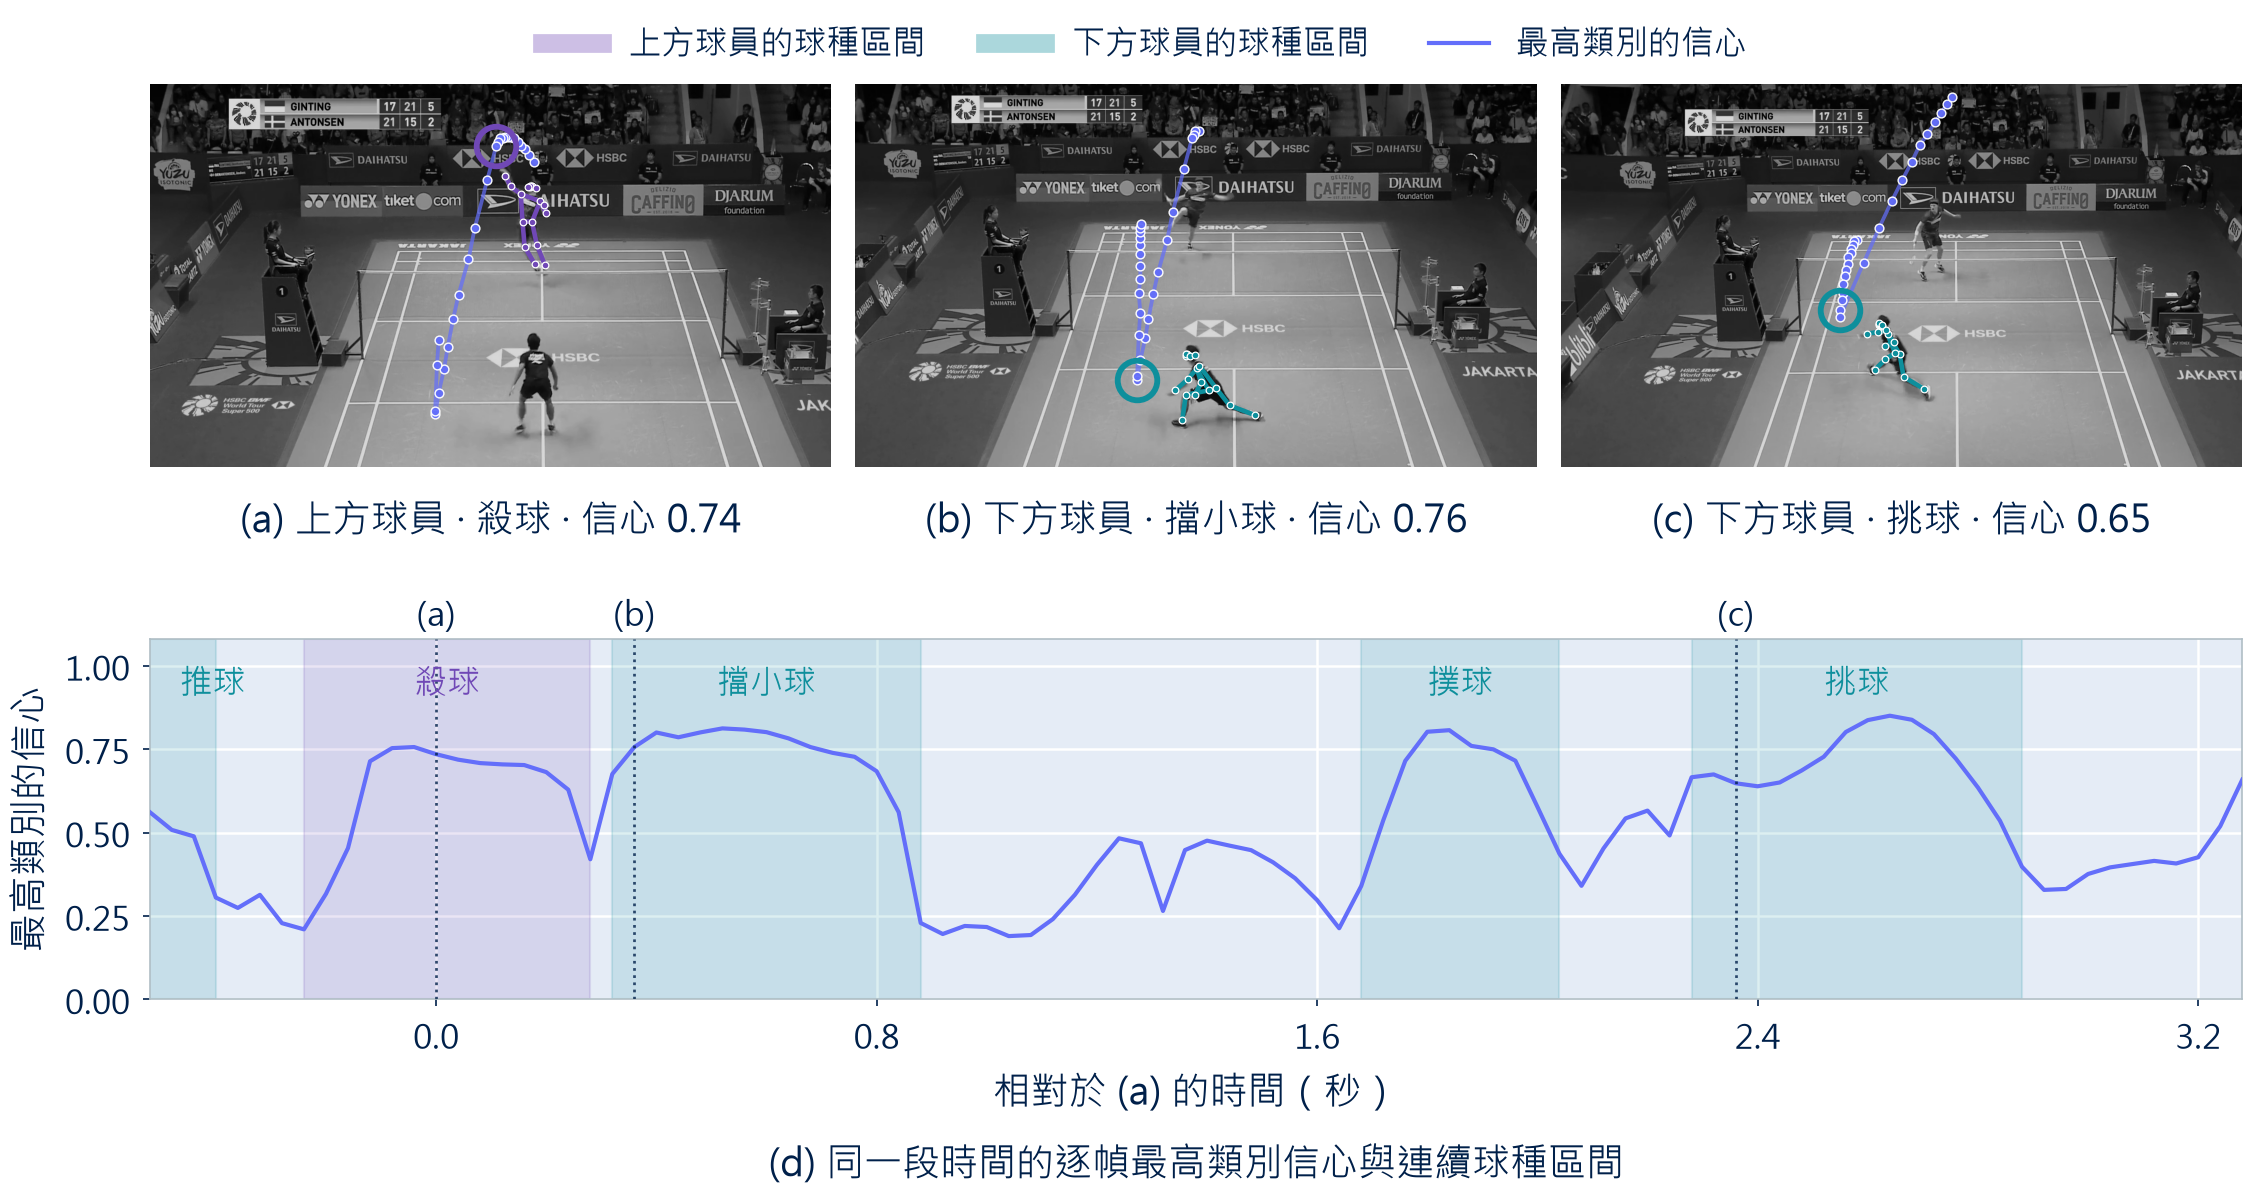
\includegraphics[width=\linewidth]{event_detection/dense_evidence.png}
  \caption{逐幀滑動窗口產生的球種、信心與擊球者證據}
  \label{fig:dense-evidence}
\end{figure}

\subsubsection{候選生成}

本步驟分析軌跡中實際存在的有效點。由於不同球種在軌跡上的差異很大，不同位置擊球也會造成軌跡產生不同變化，因此單一訊號無法抓出所有擊球。本步驟尋找下列互補的擊球特徵（\figref{fig:candidate-signals}）：

\textbf{垂直轉折：}影像座標的 $y$ 值向下增加，因此羽球下降至球員附近、擊球後重新上升時，會在軌跡上形成局部最大值。

\textbf{方向與速率突變：}比較候選前後的速度向量，若方向明顯轉折且速率比例突然改變，較可能是球拍接觸，而非重力造成的平順轉彎。

\textbf{由慢轉快：}平抽或快速推球未必形成明顯垂直轉折，因此另以擊球前後的速率比及水平速度變化尋找候選。

\textbf{發球錨點：}額外偵測回合開頭的陡峭垂直變化與第一段持續上升軌跡，作為發球候選。

本步驟刻意偏向敏感、高召回，先保留不確定候選，再交由後續規則排除（\figref{fig:candidate-pool}）。擊球時刻要用來為下一階段的球種模型切分析窗口，一旦漏掉一拍，窗口就會整段錯位，後續的比賽脈絡也會出現難以復原的斷點。

\begin{figure}[H]
  \centering
  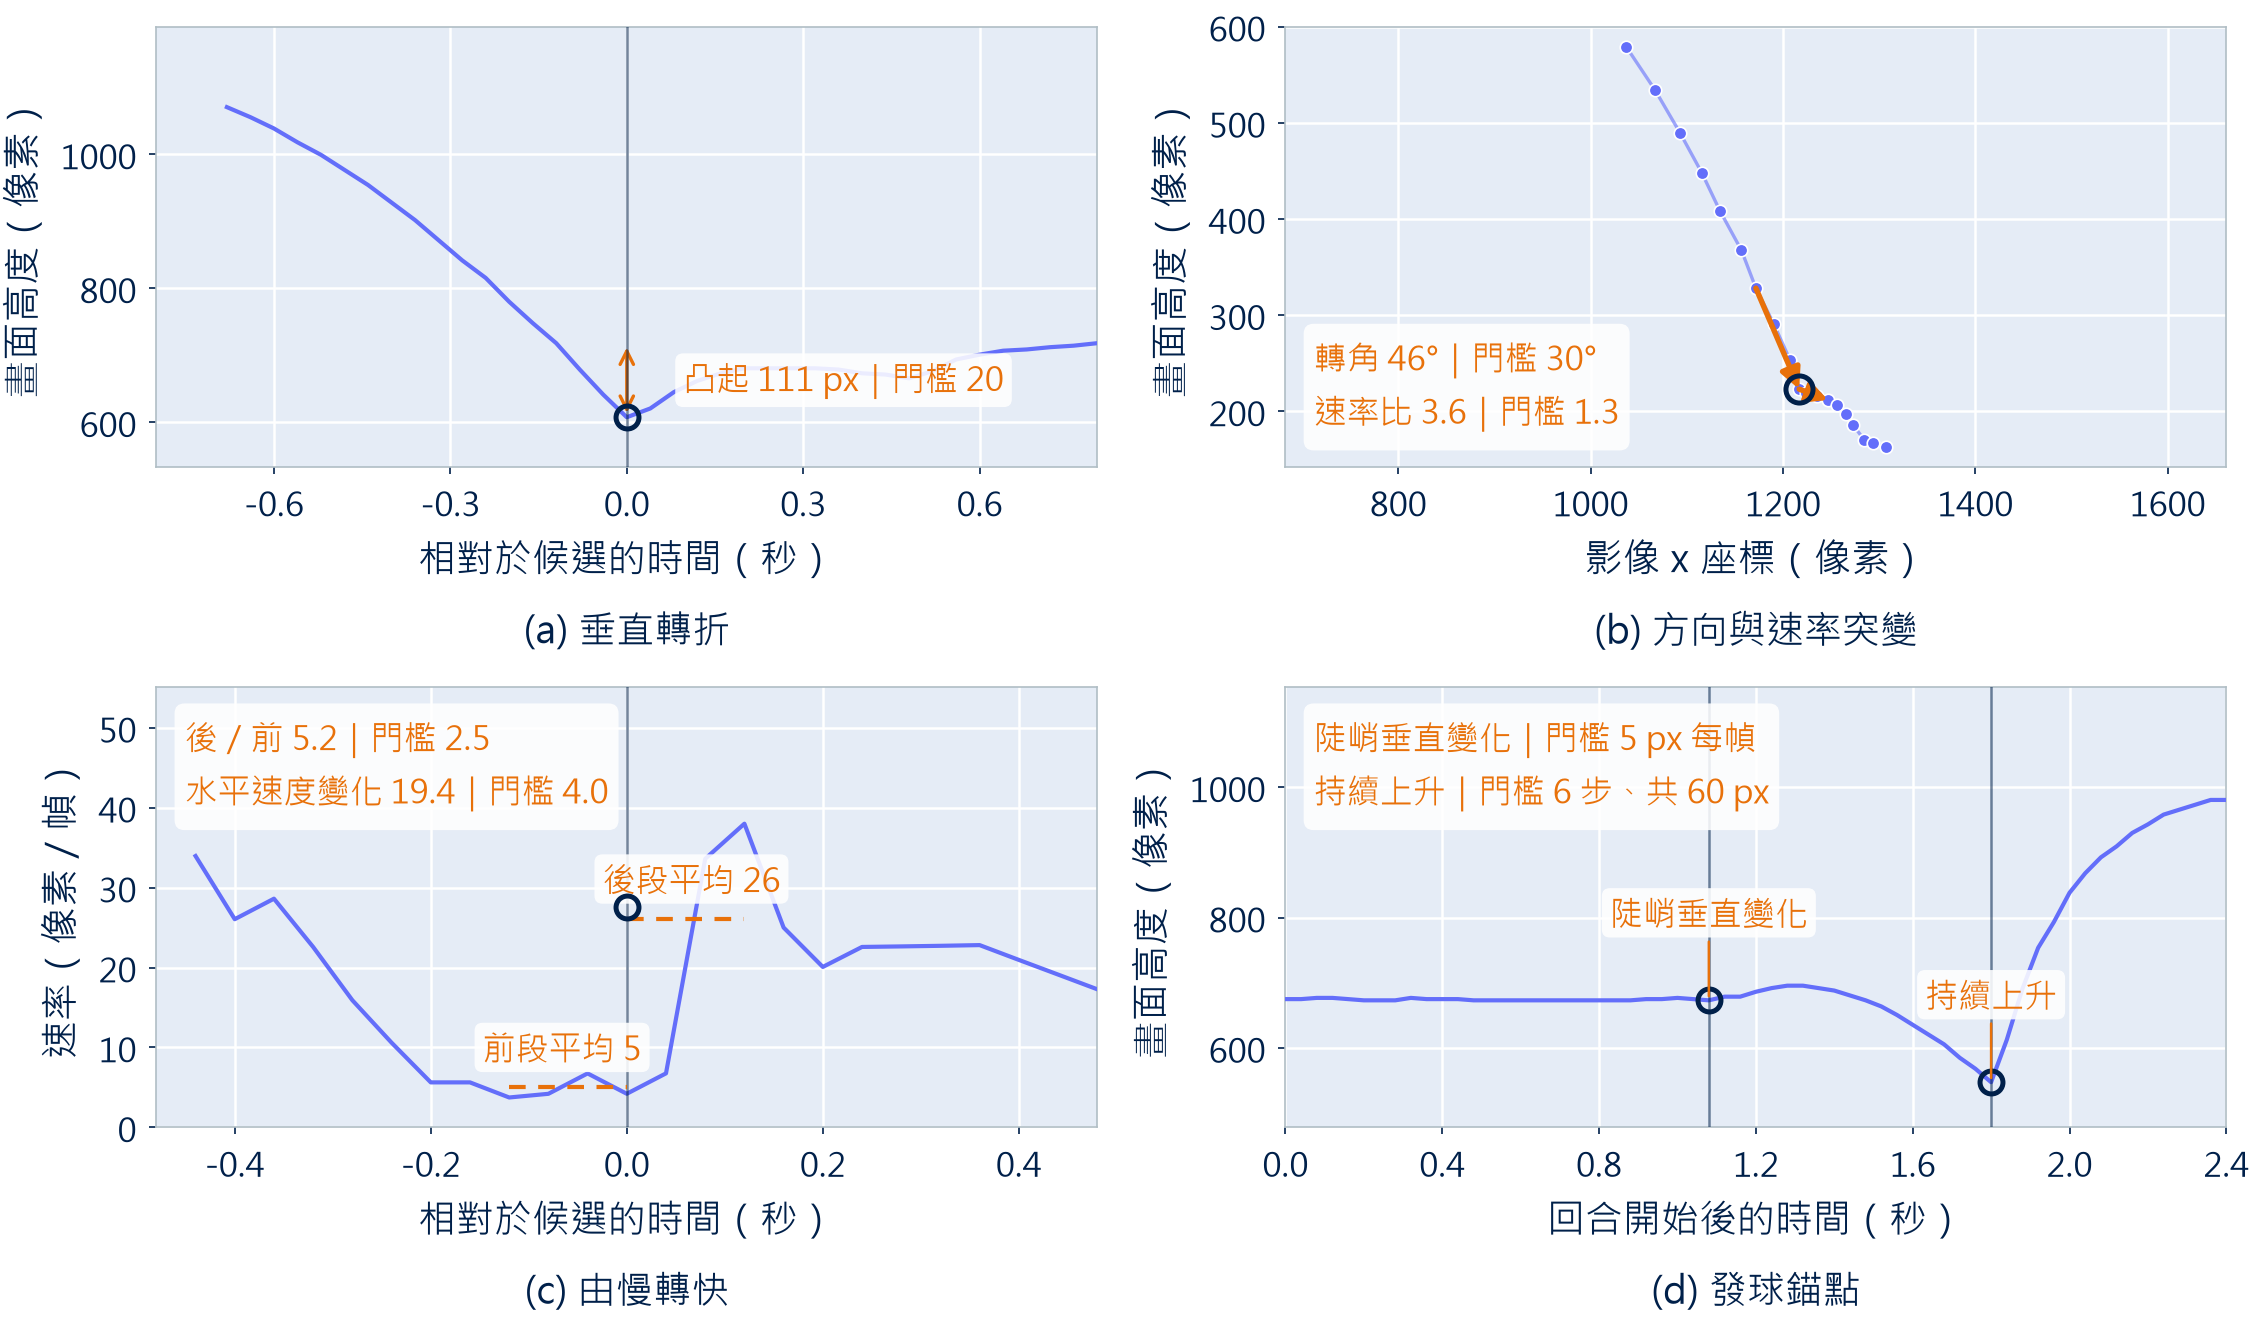
\includegraphics[width=\linewidth]{event_detection/candidate_signals.png}
  \caption{四種互補的擊球候選訊號}
  \label{fig:candidate-signals}
\end{figure}

\begin{figure}[H]
  \centering
  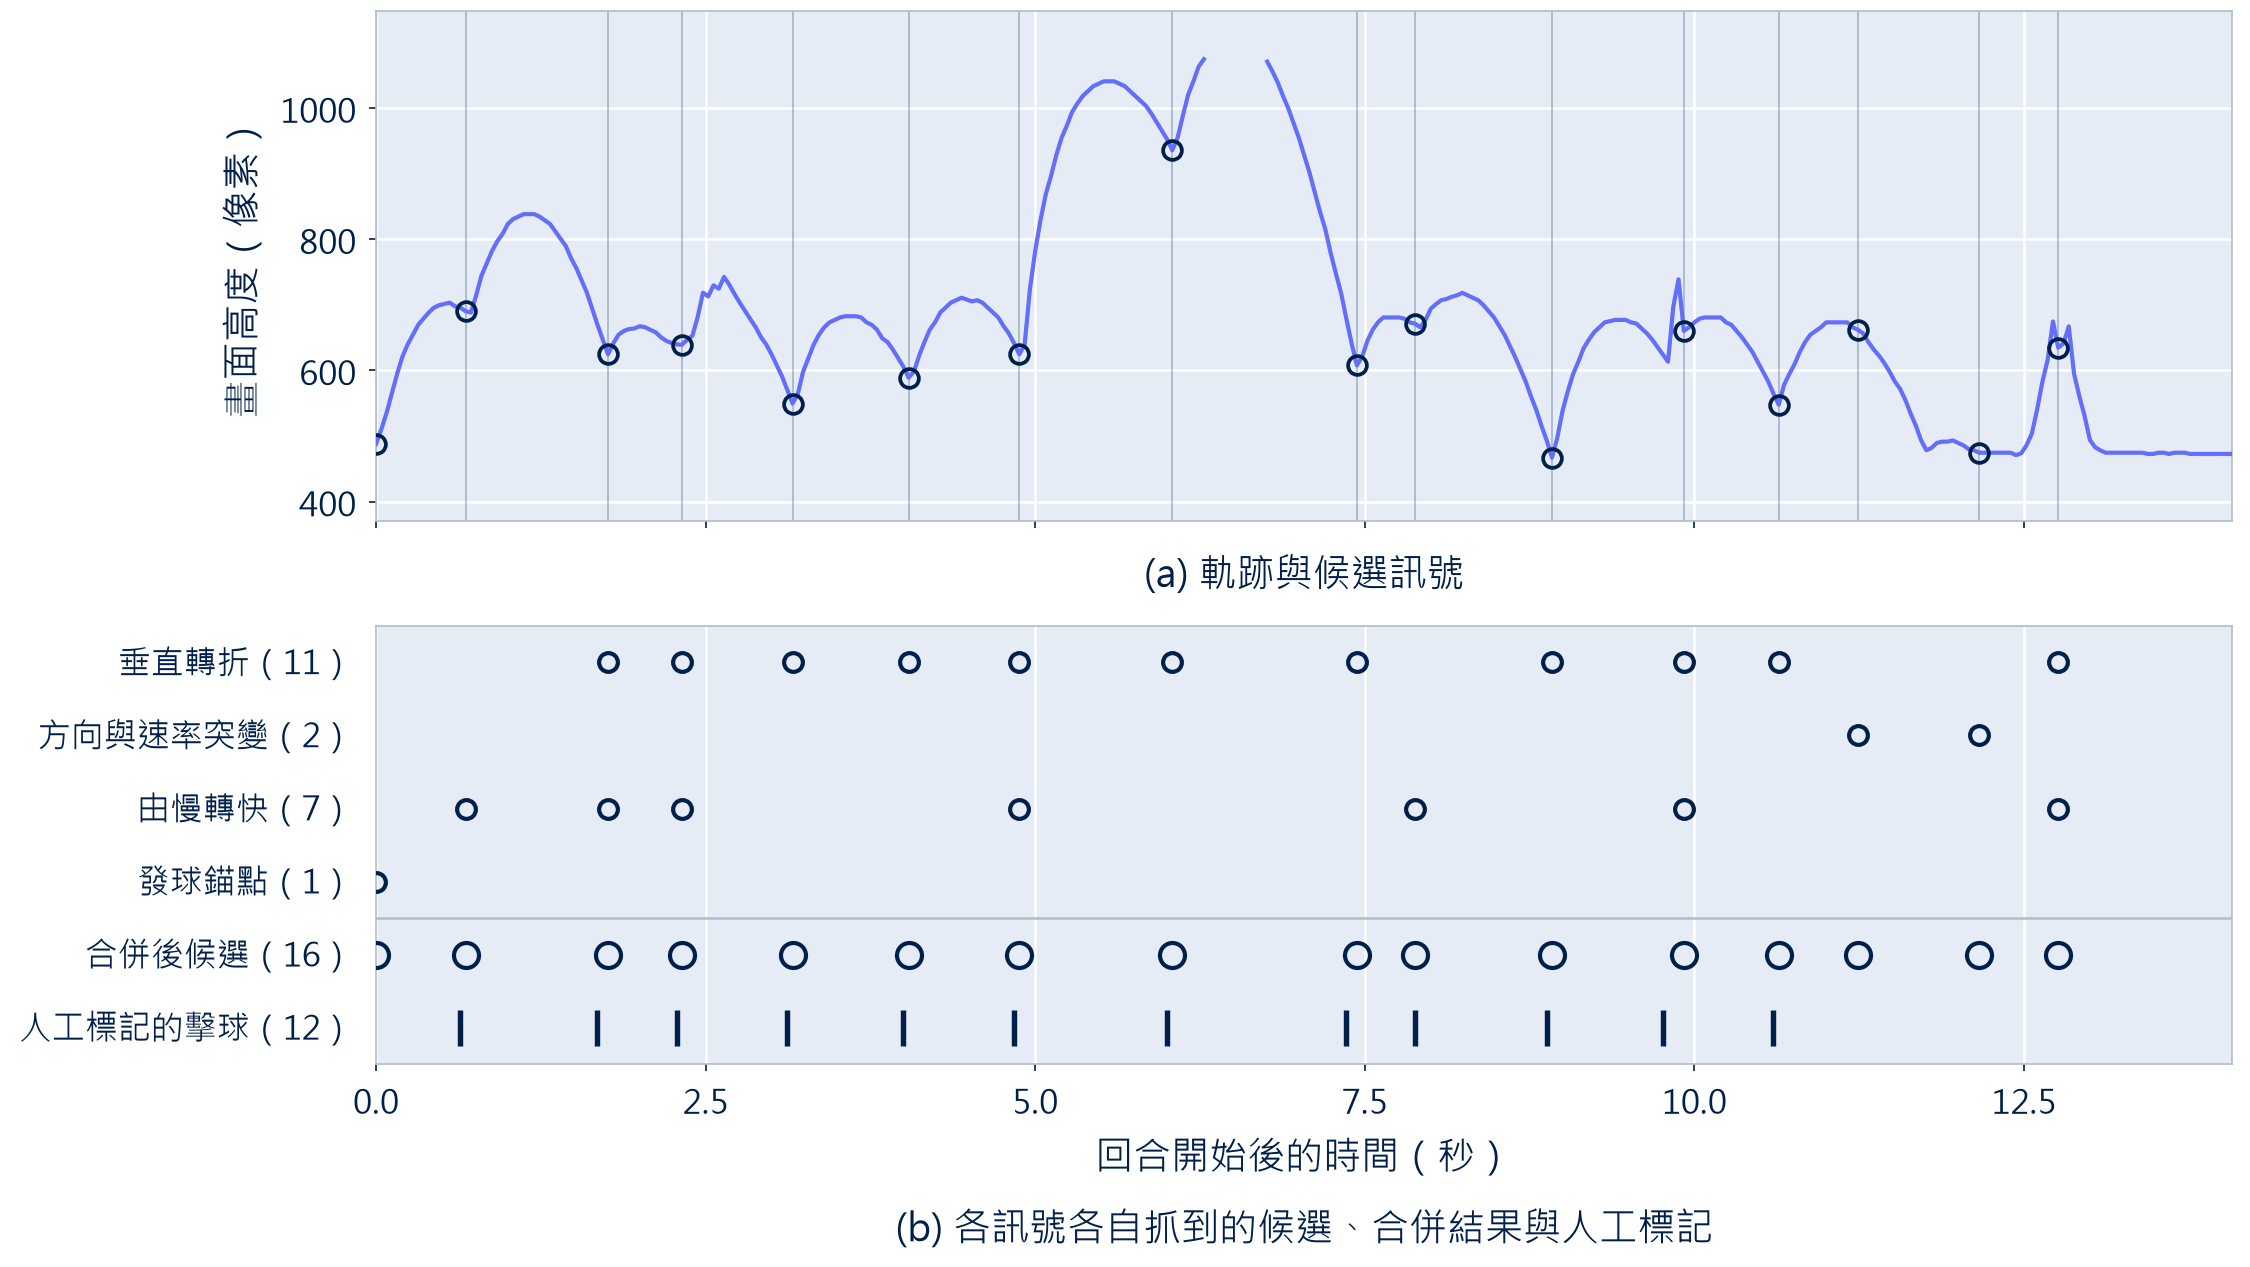
\includegraphics[width=\linewidth]{event_detection/candidate_pool.png}
  \caption{各訊號在完整回合中的候選分布與合併結果}
  \label{fig:candidate-pool}
\end{figure}

\subsubsection{候選篩選}

本步驟將候選經過三道篩選（\figref{fig:candidate-gates}）：

\textbf{位移振幅：}計算候選附近時間窗內的水平與垂直位移範圍，只要其中一軸具有足夠位移便予以保留，以排除球落地後的微小追蹤抖動。

\textbf{同球員去重：}依靠 BST 的輸出判定擊球者，若時間相近的連續候選被判為同球員擊球，通常代表一次擊球同時觸發多種軌跡訊號。系統只保留水平與垂直位移振幅總和較大的候選。

\textbf{回合脈絡：}已知擊球側的候選附近應能找到對側球員的其他擊球候選。目前規則要求在指定時間窗內至少存在兩個對側候選，否則將其視為落地彈跳、追蹤脫線或其他孤立訊號。

\begin{figure}[H]
  \centering
  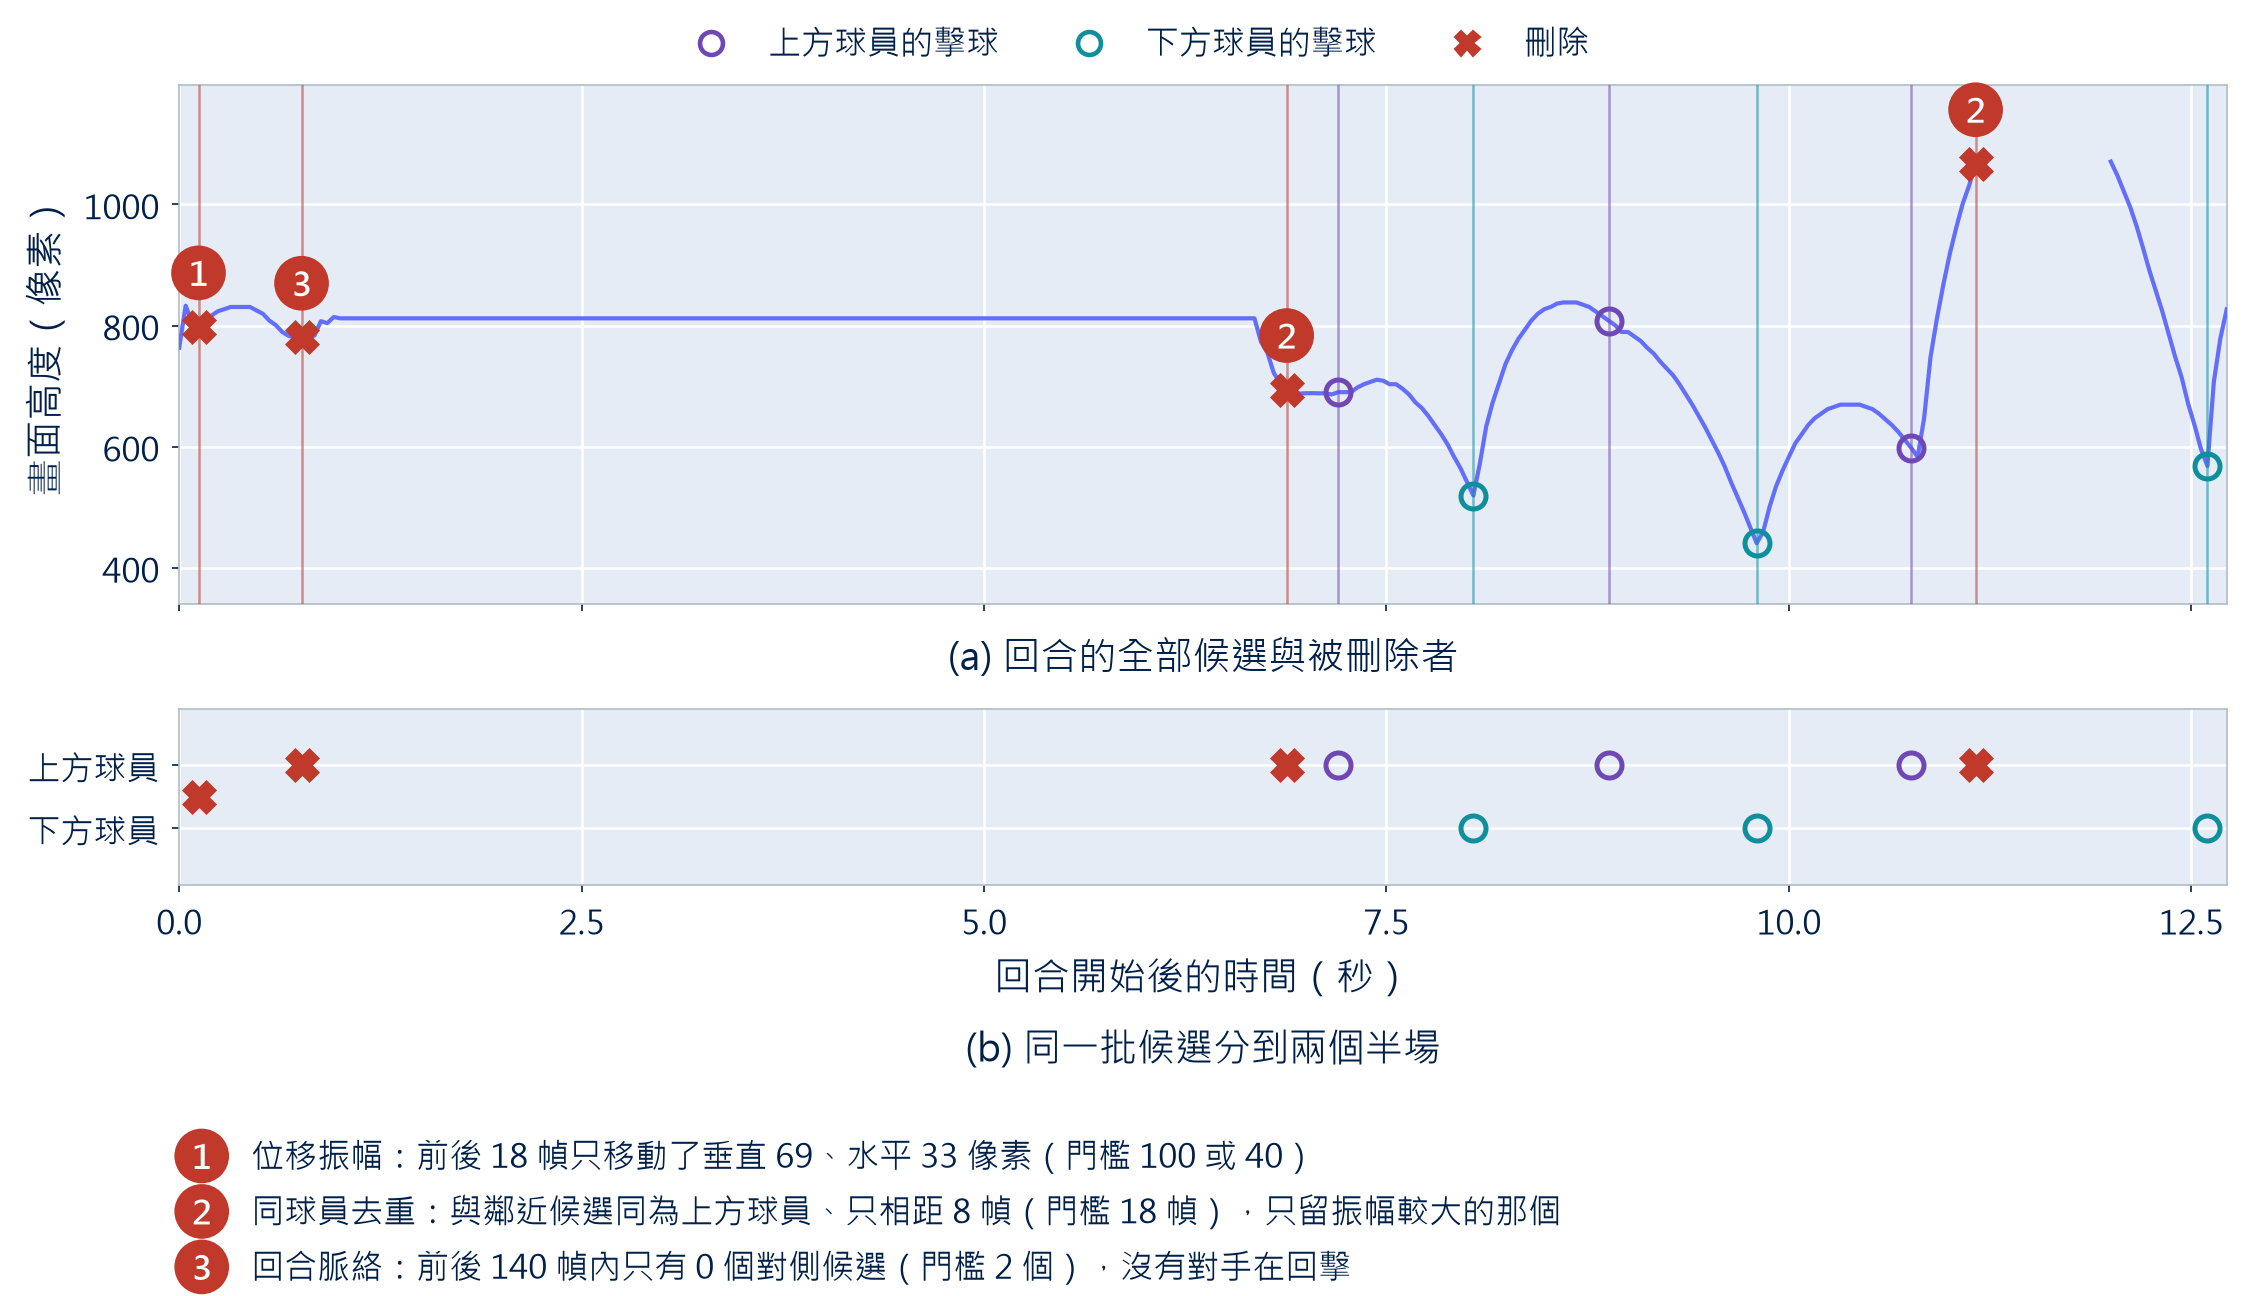
\includegraphics[width=\linewidth]{event_detection/candidate_gates.png}
  \caption{三道候選篩選規則及其保留／刪除結果}
  \label{fig:candidate-gates}
\end{figure}

\subsubsection{結構性補漏}

單靠放寬候選門檻會同時增加大量誤判，因此本步驟只在回合結構或多源證據顯示「此處很可能漏了一拍」時加入擊球。補漏刻意安排在候選篩選之後，序列先經篩選、去除雜訊後較為乾淨，回合脈絡才判斷得準，也才能據此救回一些訊號微弱、難以直接偵測的球。四條補漏規則依序執行，且新加入的擊球不得與既有擊球過近。

\textbf{交替違規補漏：}若序列中相鄰兩拍均由同球員擊出，代表兩者之間可能漏掉一拍對側擊球。系統依序搜尋主軌跡上較弱的垂直或水平轉折，以及 BST 的對側高信心連續區間，找到足夠證據後才補一拍。

\textbf{未被認領的鎖定區間：}若 BST 長時間、高信心地維持同一球種，但附近沒有任何擊球，系統會在該區間內尋找通過振幅條件的弱垂直轉折（\figref{fig:fill-sequence}）。BST 在此只指出可能漏拍的區域，不單獨決定擊球影格。

\textbf{輔助軌跡救援：}球體追蹤模組除了主軌跡，另輸出一條 Viterbi 軌跡（見\secref{sec:shuttle-tracking}），能看到主軌跡因遮擋或過度平滑而漏掉的球。若這條輔助軌跡在某處偵測到候選，且該候選接近 BST 球種訊號的起點、具有足夠信心，便將它加入。

\textbf{近端發球補漏：}畫面下方球員發球時，部分軌跡可能被身體遮擋。若持續上升錨點附近尚無擊球，而 BST 同時提供下方球員的發球證據，系統便在附近被篩掉的候選中選擇最接近者（\figref{fig:fill-trajectory}）。

\begin{figure}[H]
  \centering
  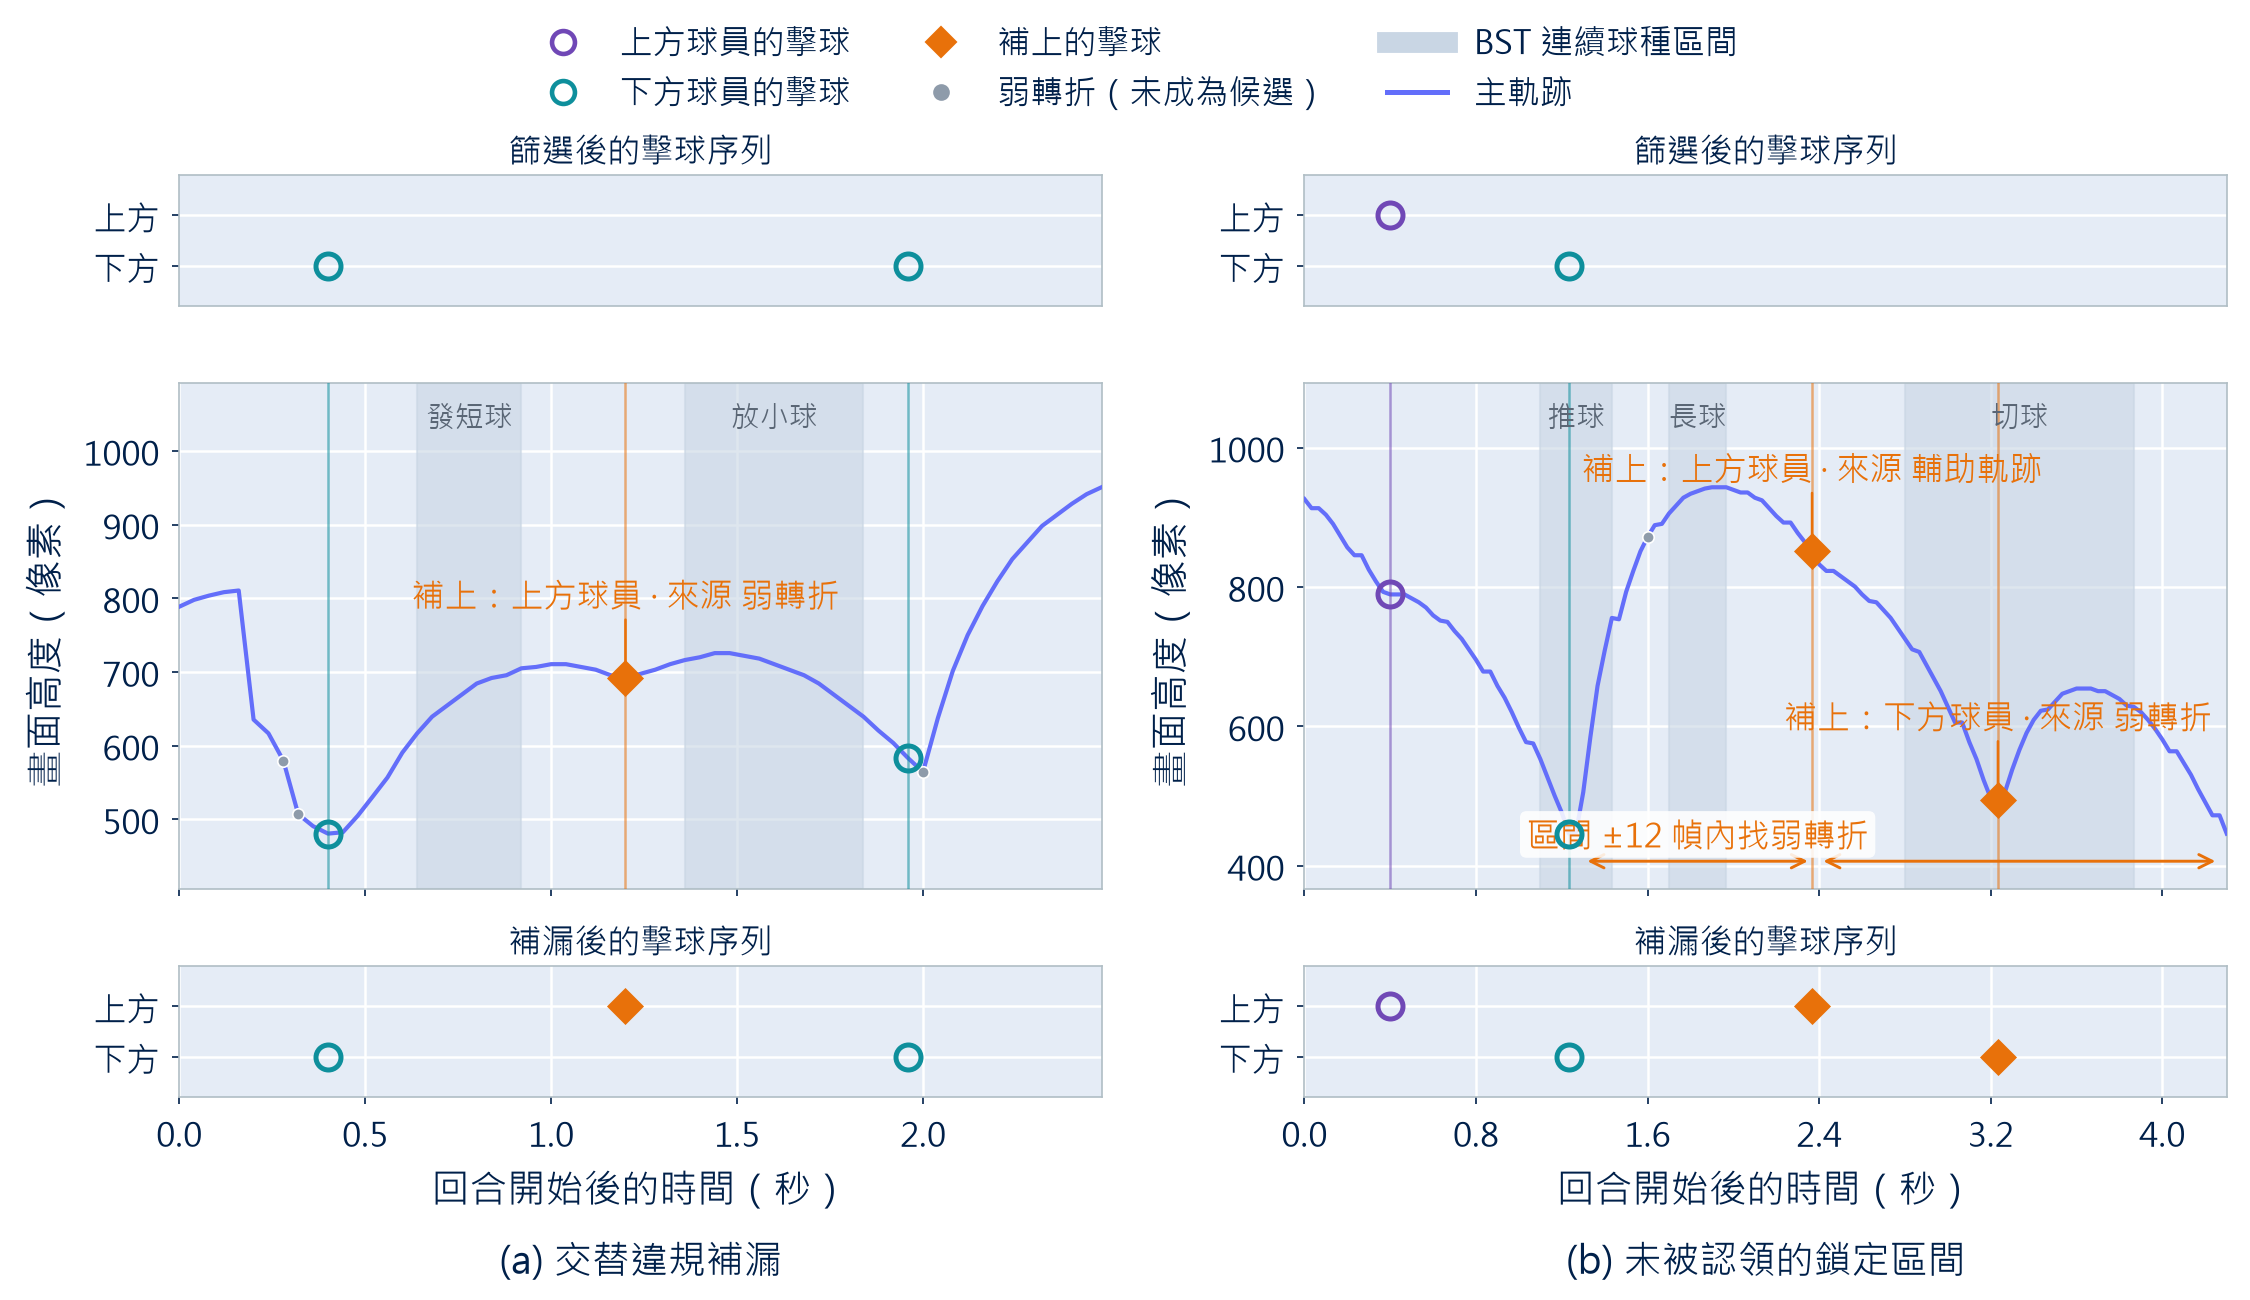
\includegraphics[width=\linewidth]{event_detection/fill_sequence.png}
  \caption{由擊球序列與連續球種證據反推漏拍位置}
  \label{fig:fill-sequence}
\end{figure}

\begin{figure}[H]
  \centering
  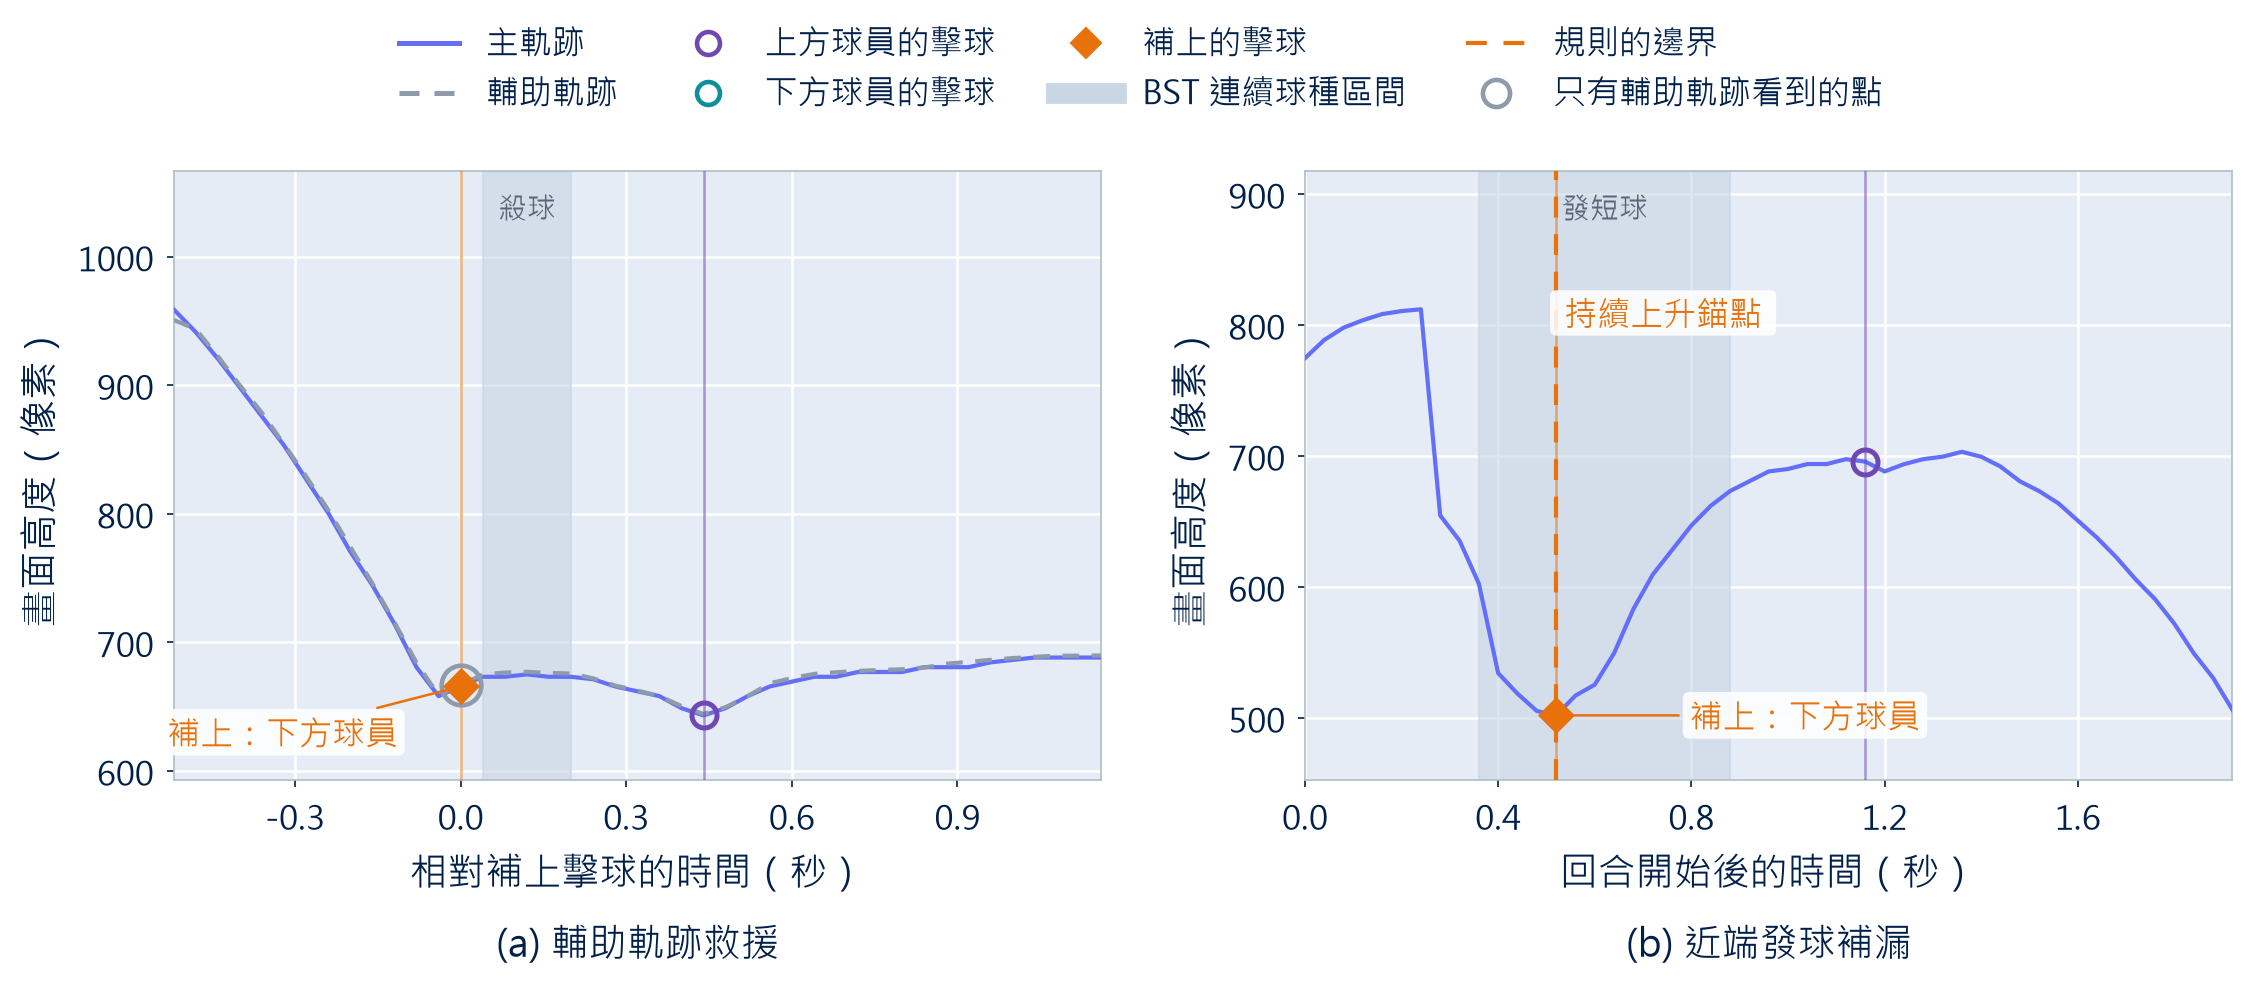
\includegraphics[width=\linewidth]{event_detection/fill_trajectory.png}
  \caption{由輔助軌跡與發球錨點救回漏拍}
  \label{fig:fill-trajectory}
\end{figure}

\subsubsection{誤判修剪}

本步驟清理回合邊緣不屬於實際對打的少數雜訊。僅針對三種很特定、平時不常觸發的情況：

\textbf{回合有效區間：}發球前場上還沒有球在移動，球體追蹤可能把反光亮點之類誤認成球，生出不存在的球路，需剔除。

\textbf{尾段落地球：}回合結束後，羽球的彈跳與滾動仍可能產生軌跡轉折，需剔除（\figref{fig:prune-rally-edges}）。

\textbf{計分板死時間：}特定休息比分下的計分板死時間（如開局 0:0、局中技術暫停，\figref{fig:prune-scoreboard}）。

\begin{figure}[H]
  \centering
  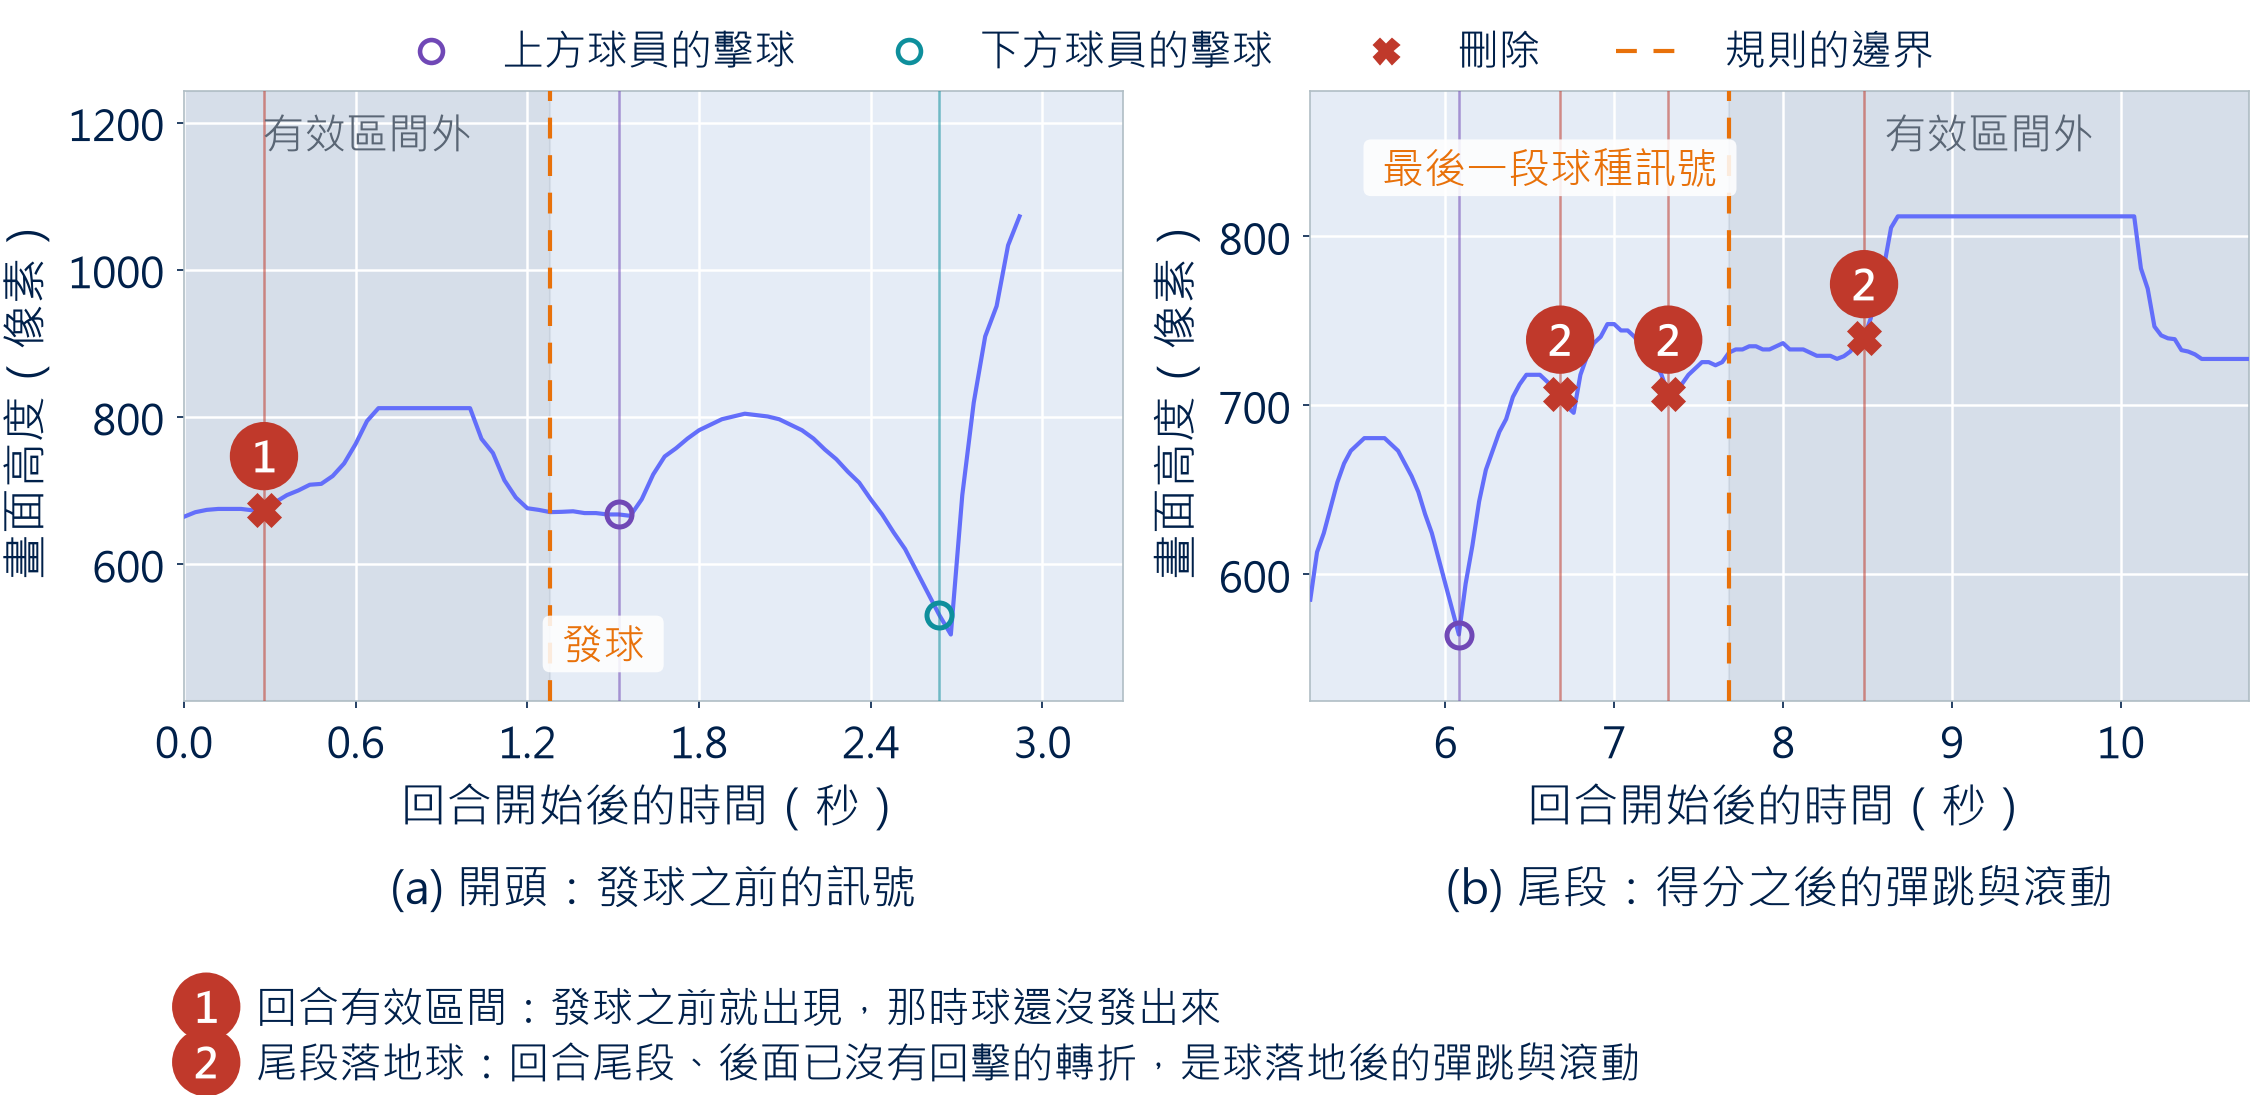
\includegraphics[width=\linewidth]{event_detection/prune_rally_edges.png}
  \caption{利用回合有效邊界清除開頭誤偵與尾段落地球}
  \label{fig:prune-rally-edges}
\end{figure}

\begin{figure}[H]
  \centering
  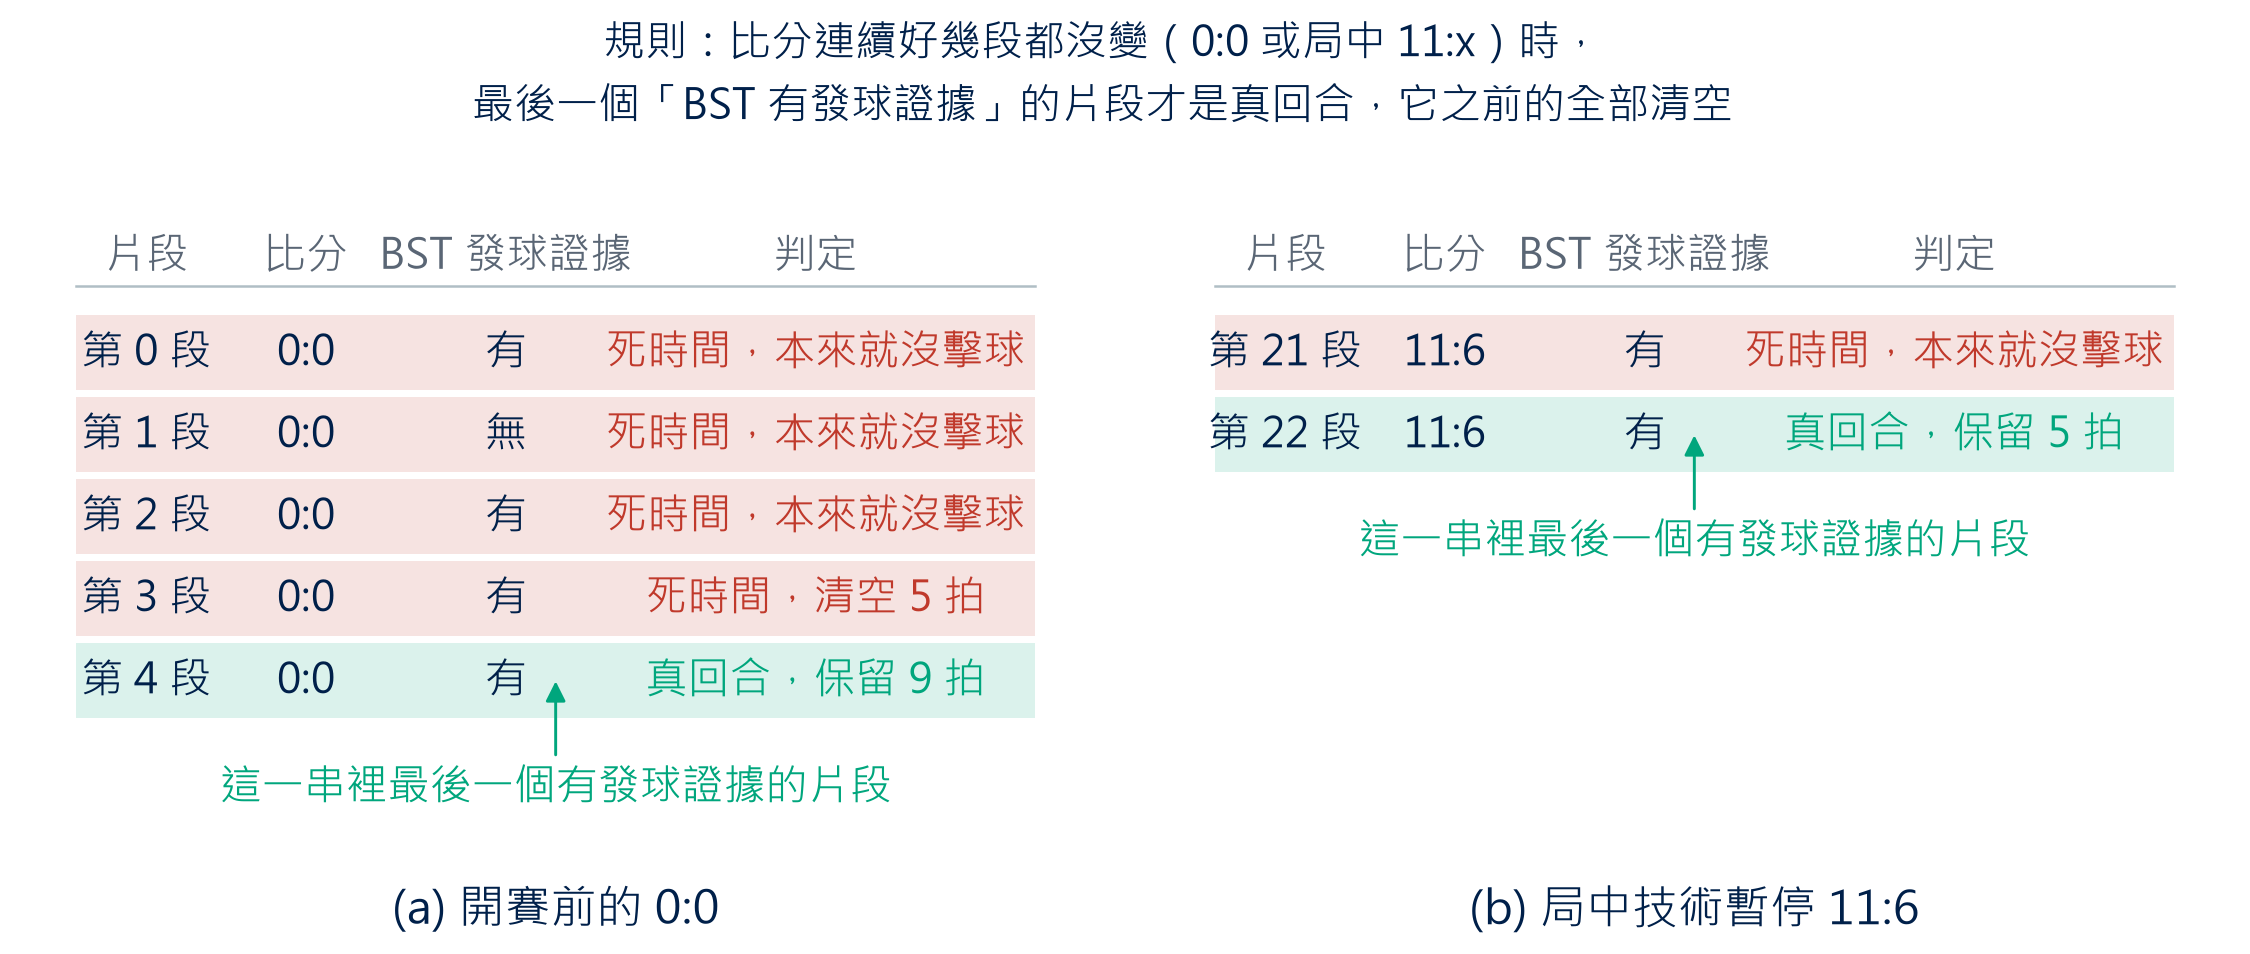
\includegraphics[width=\linewidth]{event_detection/prune_scoreboard.png}
  \caption{結合比分與發球證據判定計分板死時間}
  \label{fig:prune-scoreboard}
\end{figure}

\subsection{球種分類}
\label{sec:stroke-classification}

\subsubsection{概述}

\textbf{問題與目標：}本階段根據每一次擊球前後的球員姿態、場上位置與羽球軌跡，判斷擊球者及球種。

\textbf{設計重點：}球種分類器採用預訓練的 Badminton Stroke-type Transformer（BST）~\cite{bst}，本專題不重新訓練或修改其模型架構。BST 解決的是「已知擊球時刻及各項特徵後，如何判斷球種」。本專題在球種分類上的重點在於，利用前述各模組，自動從原始比賽影片產生 BST 所需的全部輸入。

\textbf{處理流程總覽：}如\figref{fig:stroke-classification-flow}。

\begin{figure}[H]
  \centering
  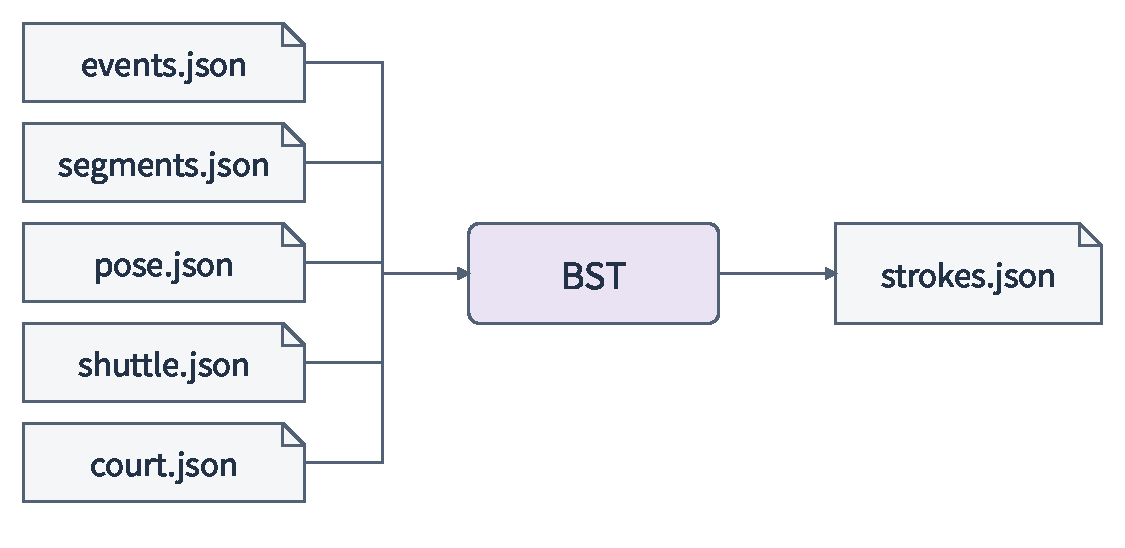
\includegraphics[scale=\flowscale]{stroke-classification.pdf}
  \caption{球種分類處理流程}
  \label{fig:stroke-classification-flow}
\end{figure}

\subsubsection{分類流程}

系統先將每個擊球時刻歸入對應回合，再依 BST 預訓練權重所使用的方式，以相鄰擊球時刻切出分析窗口。窗口內的球員骨架、場上位置與羽球軌跡會按照 BST 的資料格式進行正規化，並統一整理為 100 幀的輸入序列（\figref{fig:bst-window}）。

整理後的資料送入預訓練 BST，模型輸出 25 類機率（\figref{fig:bst-output}），將結果依賽評需求整理為 8 類：高遠球、發球、小球、平快球、殺球、切球、撲球與勾球。若模型輸出未知類別，系統保留為未知。

\begin{figure}[H]
  \centering
  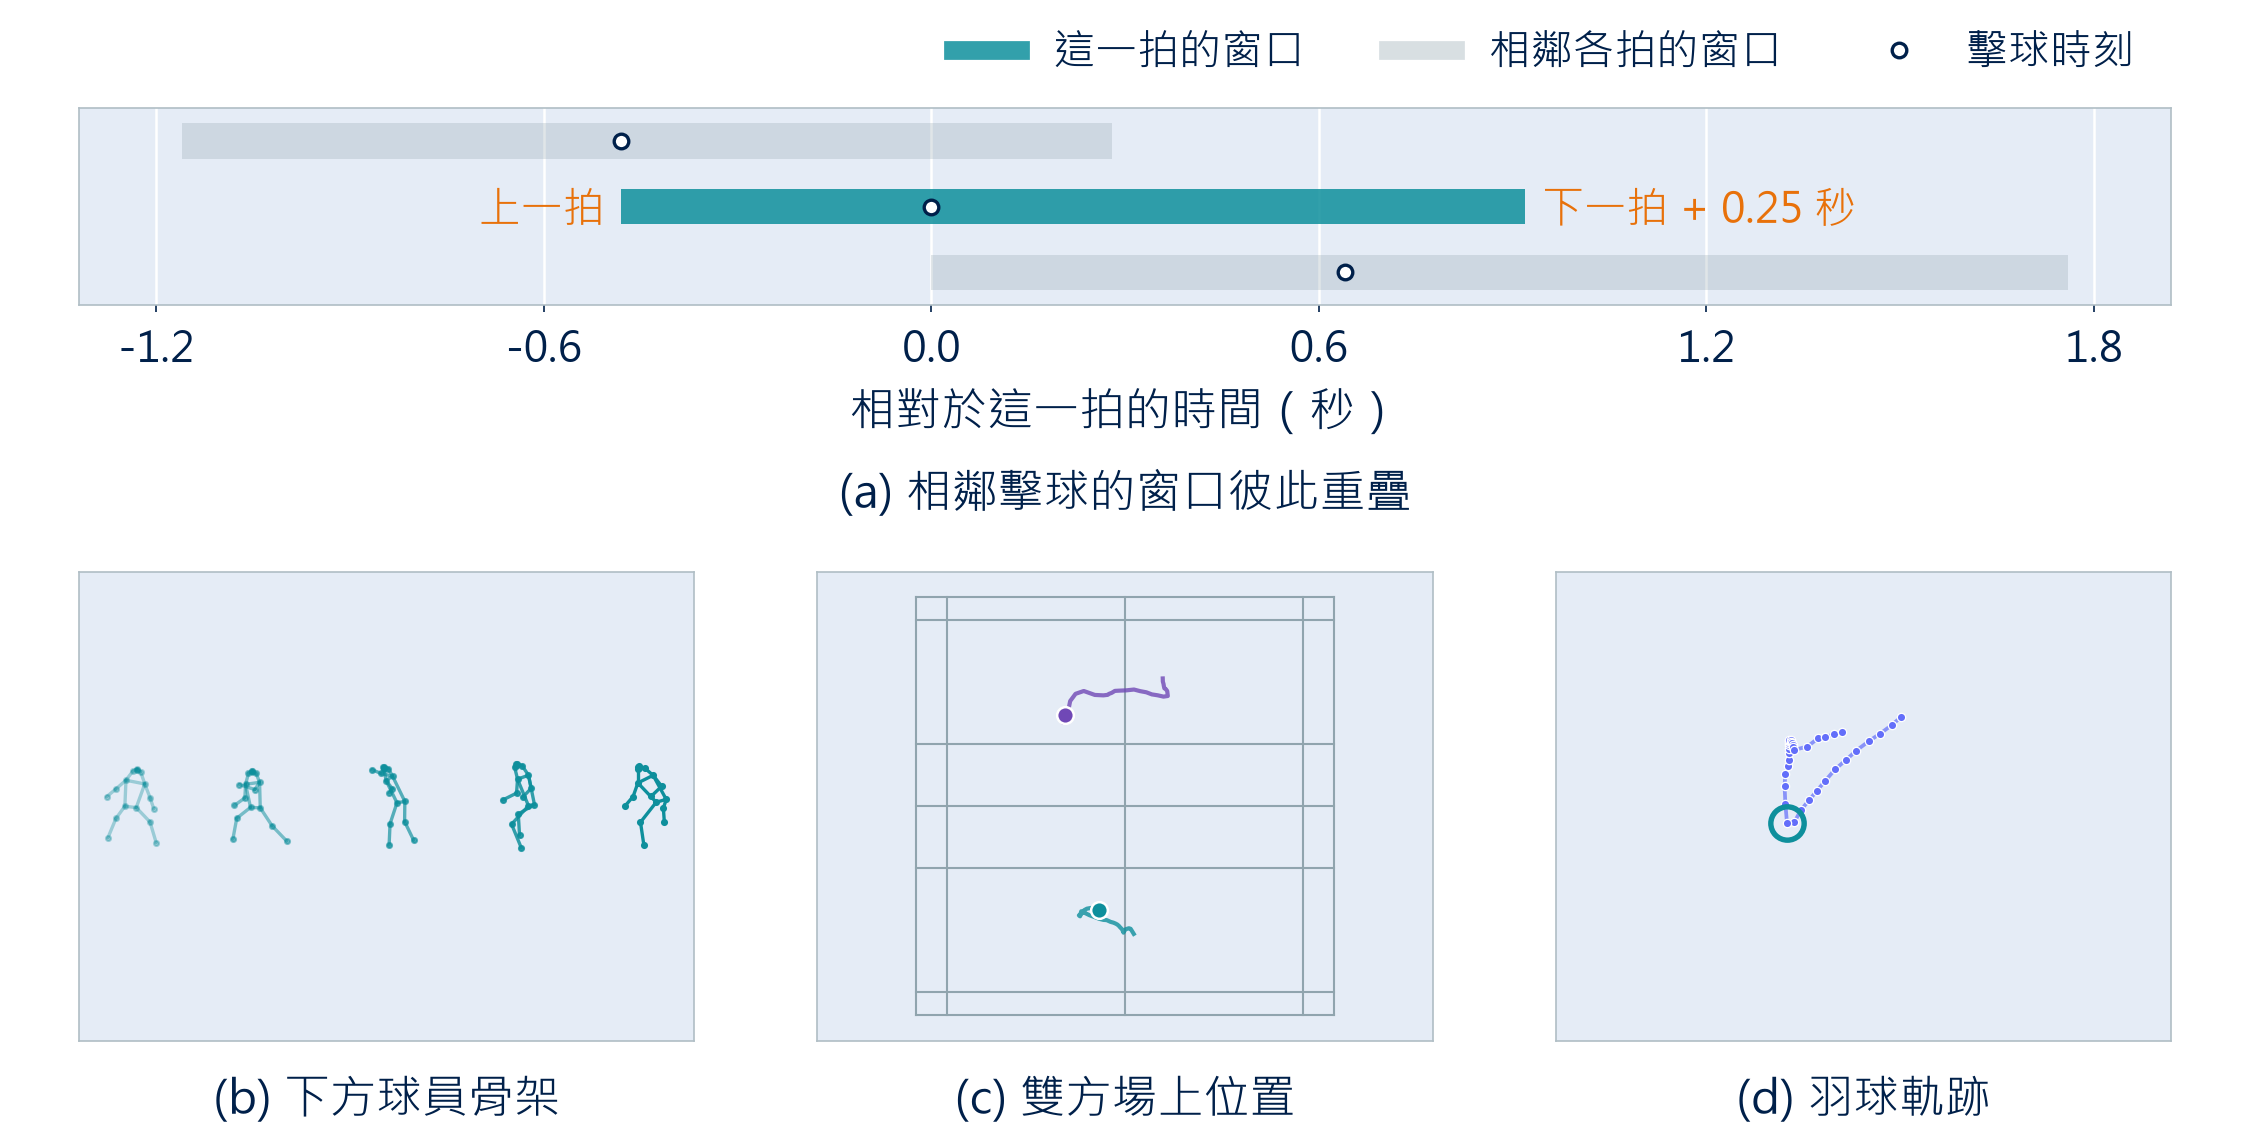
\includegraphics[width=\linewidth]{stroke_classification/bst_window.png}
  \caption{依相鄰擊球時刻建立 BST 的 100 幀輸入窗口}
  \label{fig:bst-window}
\end{figure}

\begin{figure}[H]
  \centering
  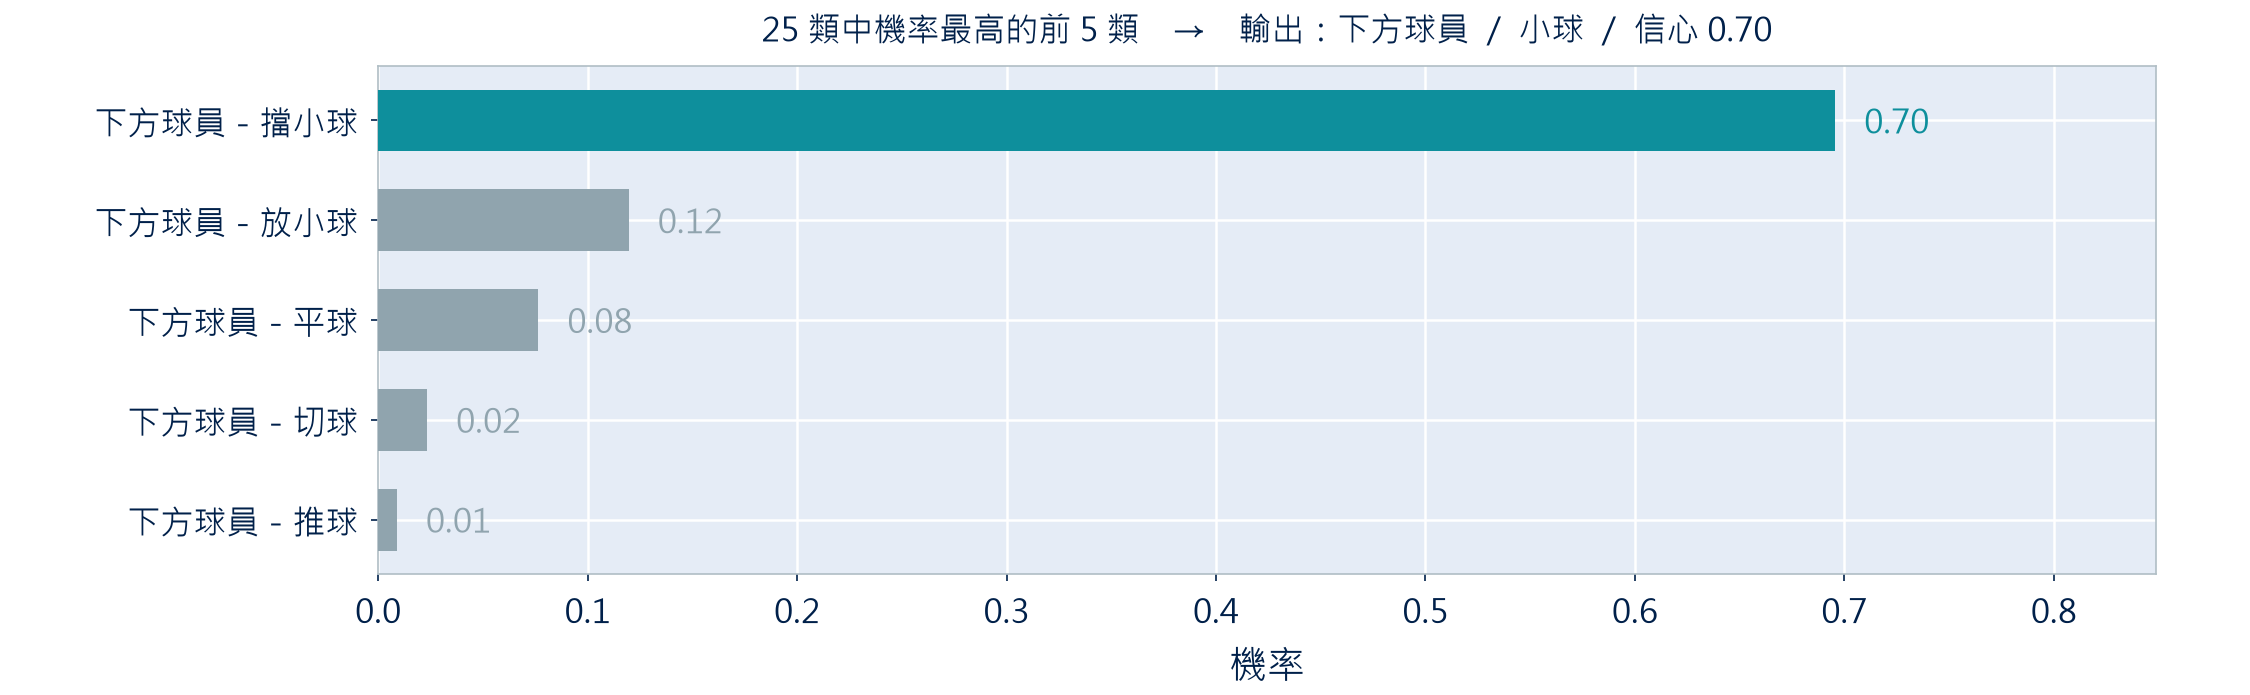
\includegraphics[width=\linewidth]{stroke_classification/bst_output.png}
  \caption{BST 的 25 類預測}
  \label{fig:bst-output}
\end{figure}

\section{音訊與精彩度分析}
\label{sec:audio-highlights}

\subsection{歡呼音訊量測}
\label{sec:cheer-audio}

\subsubsection{概述}

\textbf{問題與目標：}視覺模組能說明每一拍發生了什麼，卻無法判斷哪個回合最讓現場有反應。觀眾歡呼是轉播中現成的精彩度訊號。本模組以分段模組產生的每個片段為範圍，量測片段結束前後是否出現歡呼及其相對強度，作為精彩片段排序的依據。

\textbf{設計重點：}本模組不從頭訓練音訊模型，而是以凍結的 YAMNet~\cite{yamnet} 擷取通用音訊特徵，只在其上訓練一個輕量的邏輯迴歸分類器，因此 400 個人工標註窗口就足以完成訓練。歡呼多在回合結束的瞬間爆發，所以讀取範圍會延伸到片段結束後 3 秒。分類與強度分開估計：分類器判斷窗口裡有沒有歡呼，響度則衡量歡呼有多大聲，兩者再各自聚合為每個片段一筆量測。音訊只是視覺分析的補充，不建立或覆寫擊球、球種、比分與球員身分等競賽事實，缺少音訊時，其餘模組仍照常運作。以 4 場比賽逐場交叉驗證，窗口層級歡呼偵測的 macro F1 為 0.827、ROC-AUC 為 0.957（見\secref{sec:exp-cheer}）。

\textbf{處理流程總覽：}如\figref{fig:audio-cheer-flow}。

\begin{figure}[H]
  \centering
  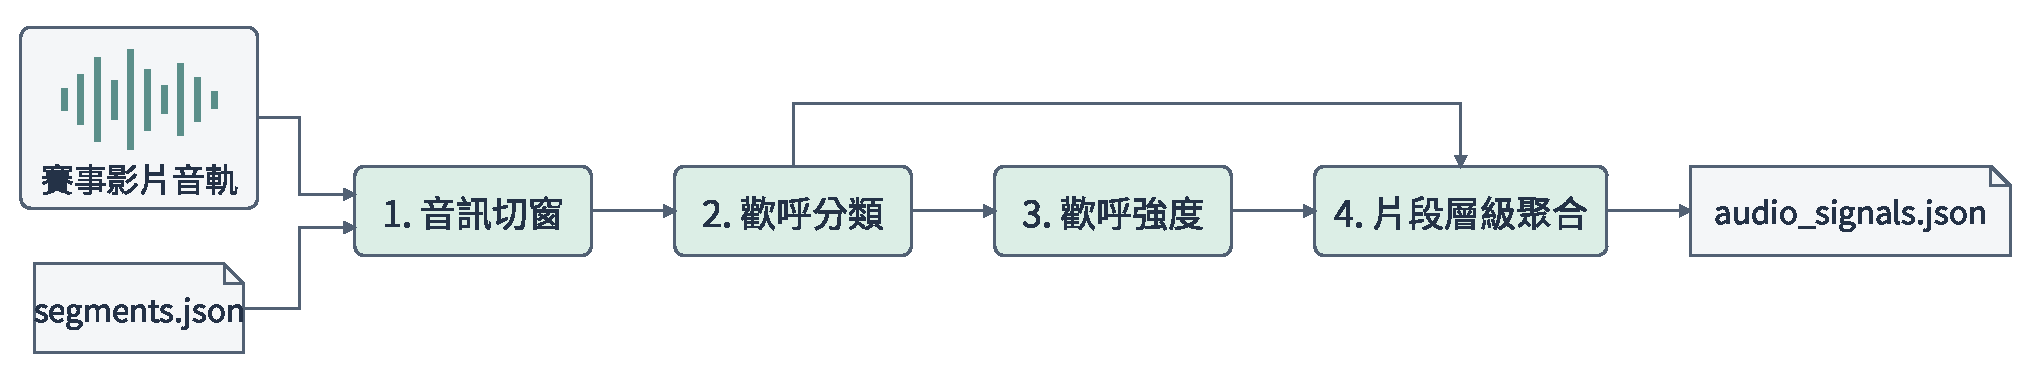
\includegraphics[scale=\flowscale]{audio-cheer.pdf}
  \caption{歡呼音訊量測處理流程}
  \label{fig:audio-cheer-flow}
\end{figure}

\subsubsection{音訊切窗}

系統先將音訊統一轉為 16 kHz 單聲道。對片段 $s$，分析起點等於片段起點，終點則延伸到片段結束後 3 秒，並以影片長度為上限：
\begin{equation}
  A_s^{start}=S_s^{start},\qquad
  A_s^{end}=\min(S_s^{end}+3,\;T_{media})
\end{equation}
延伸的原因是歡呼往往在回合結束時才開始，並在片段結束後持續數秒。分析範圍以 3 秒窗口切分，相鄰窗口的 hop 為 1 秒，只保留完整落在範圍內的窗口，尾端不足 3 秒的窗口直接捨棄（\figref{fig:audio-windows}）。相鄰片段各自切窗，因此兩者的窗口可能重疊。

\begin{figure}[H]
  \centering
  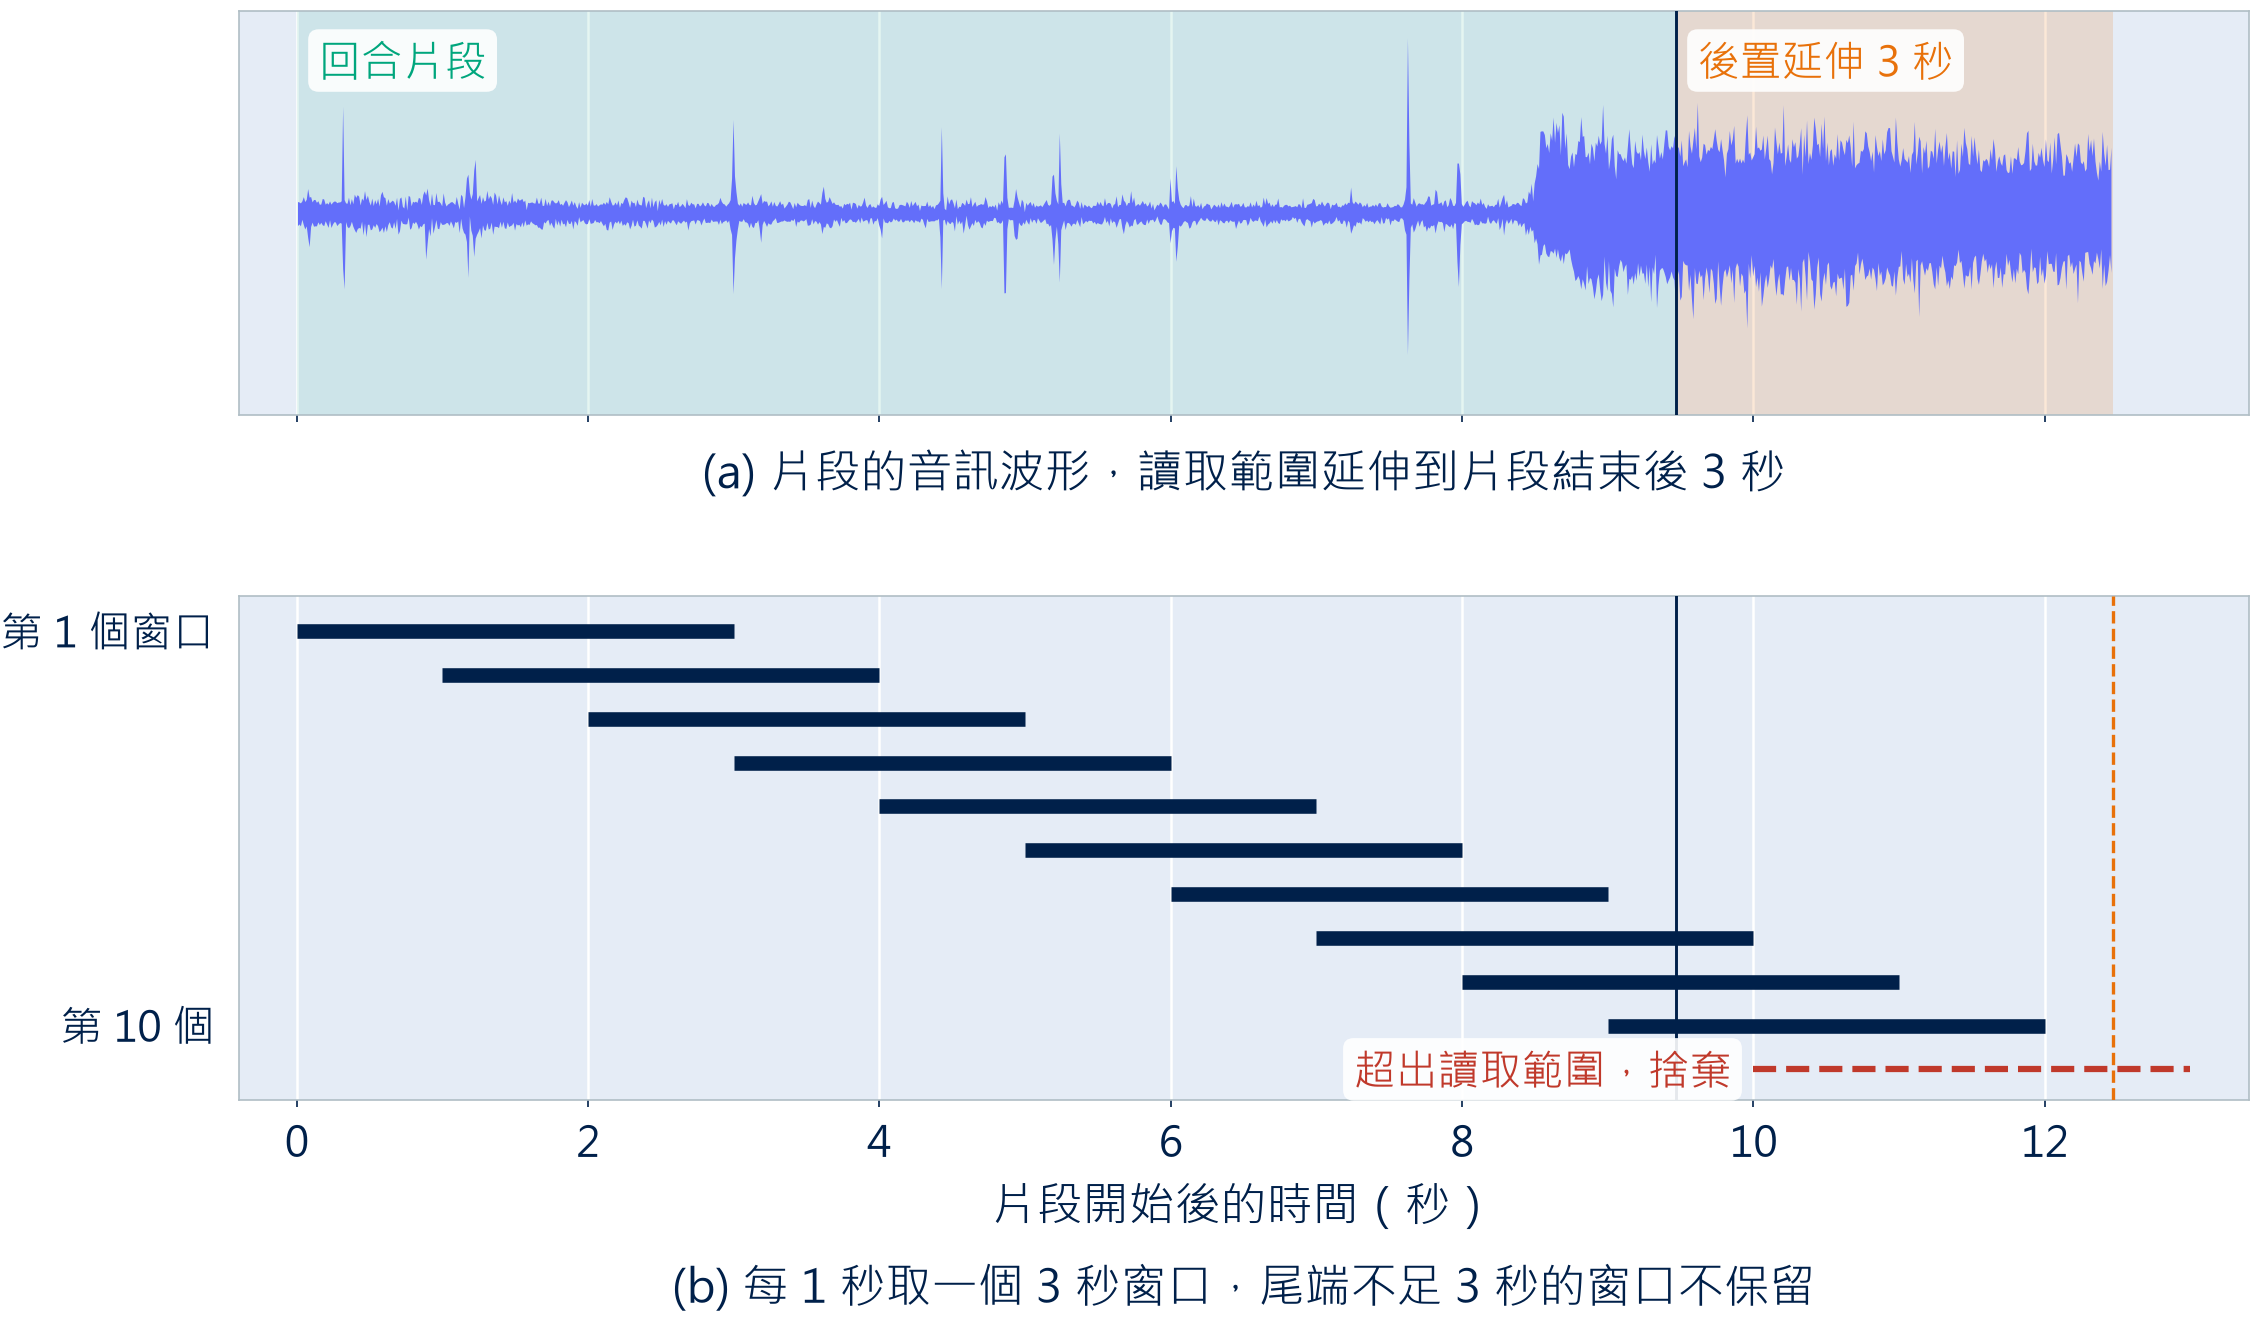
\includegraphics[width=\linewidth]{audio_highlight/audio_windows.png}
  \caption{片段音訊的讀取範圍與切窗}
  \label{fig:audio-windows}
\end{figure}

\subsubsection{歡呼分類}

每個 3 秒窗口輸入凍結的 YAMNet~\cite{yamnet}。YAMNet 以 AudioSet~\cite{audioset} 音訊事件資料預訓練，對一個窗口輸出多個時間切片的 1024 維特徵向量（patch embedding），系統取其平均作為窗口的固定長度表示：
\begin{equation}
  \mathbf{e}_i=\frac{1}{K_i}\sum_{k=1}^{K_i}\mathbf{z}_{i,k},
  \qquad \mathbf{e}_i\in\mathbb{R}^{1024}
\end{equation}
其中 $\mathbf{z}_{i,k}$ 為第 $i$ 個窗口的第 $k$ 個時間切片特徵，$K_i$ 為切片數。平均向量經標準化後送入邏輯迴歸，輸出窗口的歡呼分數 $p_i\in[0,1]$；$p_i\ge 0.5$ 的窗口視為正例窗口。

本系統不直接使用 YAMNet 原生的 Cheering 類別分數。在相同的逐場交叉驗證下，原生分數的 ROC-AUC 只有 0.839，以特徵向量訓練的分類器則為 0.957（見\secref{sec:exp-cheer}）。歡呼分數是分類器的輸出，未經機率校準，只用於門檻判斷與排序，不應解讀為歡呼發生的機率。

\subsubsection{歡呼強度估計}

同樣被判為歡呼，全場起立的喝采與零星掌聲在響度上可能差很多。因此系統另以窗口波形 $x_1,\ldots,x_N$ 的均方根（RMS）衡量響度：
\begin{equation}
  RMS_i=\sqrt{\frac{1}{N}\sum_{n=1}^{N}x_n^2},\qquad
  L_i=20\log_{10}(RMS_i+10^{-12})
\end{equation}
不同轉播的錄音音量差異很大，絕對響度無法跨比賽比較，因此系統只在單場比賽內比較。將全場 $M$ 個正例窗口的 $L_i$ 由小到大排名（從 0 起算，同值取平均排名），再除以 $M-1$ 映射到 $[0,1]$，得到窗口的歡呼強度 $r_i$。全場只有一個正例窗口時，強度定為 0.5。負例窗口不計算強度。$r_i$ 表示這個窗口在本場所有歡呼中的響度排名，而不是實際音壓。

\subsubsection{片段層級聚合}

每個片段約有十多個窗口，需要聚合為一筆量測。歡呼通常只占片段的最後幾秒，取平均會被前段大量的安靜窗口稀釋，取最大值則容易被單一誤判窗口左右。系統因此折衷採用線性內插的第 95 百分位數（p95）。令 $W_s$ 為片段 $s$ 的全部窗口、$W_s^+$ 為其中的正例窗口：
\begin{gather}
  C_s=Q_{0.95}^{linear}(\{p_i\mid i\in W_s\}),\qquad N_s=|W_s^+| \\
  I_s=
  \begin{cases}
    Q_{0.95}^{linear}(\{r_i\mid i\in W_s^+\}), & |W_s^+|>0\\
    \mathrm{null}, & |W_s^+|=0
  \end{cases}
\end{gather}
$C_s$ 為片段歡呼分數，聚合片段內全部窗口；$I_s$ 為片段歡呼強度，只聚合正例窗口，沒有正例時為空值；$N_s$ 為正例窗口數。由於窗口彼此重疊，$N_s$ 不等於獨立的歡呼次數。各聚合方法的比較見\secref{sec:exp-aggregation}。

\subsection{精彩片段排序}
\label{sec:highlight-ranking}

\subsubsection{概述}

\textbf{問題與目標：}本模組把每個片段的歡呼量測合成一個精彩度分數，將整場比賽的片段由精彩到平淡排序，供回看介面標示重要回合，也作為賽評生成的選用背景訊號。

\textbf{設計重點：}目前沒有人工標註的精彩片段真值可供訓練，因此精彩度分數採用透明的固定公式，而不是學習得到的模型。沒有歡呼的片段，強度以 0 計：
\begin{equation}
  H_s=0.5\,C_s+0.5\,I_s^{effective},\qquad
  I_s^{effective}=
  \begin{cases}
    I_s, & I_s\neq\mathrm{null}\\
    0, & I_s=\mathrm{null}
  \end{cases}
\end{equation}
分數相同時，依片段歡呼分數、再依片段先後排序。0.5／0.5 的權重只表示等量結合「有沒有歡呼」與「歡呼多大聲」，並非最佳化的結果。由於強度是單場內的相對量，精彩度分數也只能在同一場比賽內比較。

\textbf{處理流程總覽：}如\figref{fig:highlight-ranking-flow}。

\begin{figure}[H]
  \centering
  
\includegraphics[scale=\flowscale]{highlight-ranking.pdf}
  \caption{精彩片段排序處理流程}
  \label{fig:highlight-ranking-flow}
\end{figure}

\section{賽事理解}
\label{sec:match-understanding}

\subsection{球員身分對應}
\label{sec:player-identity}

\subsubsection{概述}

\textbf{問題與目標：}球種分類只知道擊球者位在畫面上方或下方，賽評卻需要指名選手。本階段判斷在每兩次換邊之間，上下方球員各是計分板上的哪一位選手。

\textbf{設計重點：}本階段不需要人工標註，主要也不依賴球員外觀，而是由既有的兩項結果推得。比分變化指出計分板上的哪一位選手發球，回合第一拍的擊球者指出發球者在上方或下方，兩者結合即為一次對應。換邊的時間點由羽球規則決定（第一局結束、第二局結束、決勝局領先方達 11 分），只需從比分推算，不必從畫面偵測。

\textbf{處理流程總覽：}如\figref{fig:identity-mapping-flow}。

\begin{figure}[H]
  \centering
  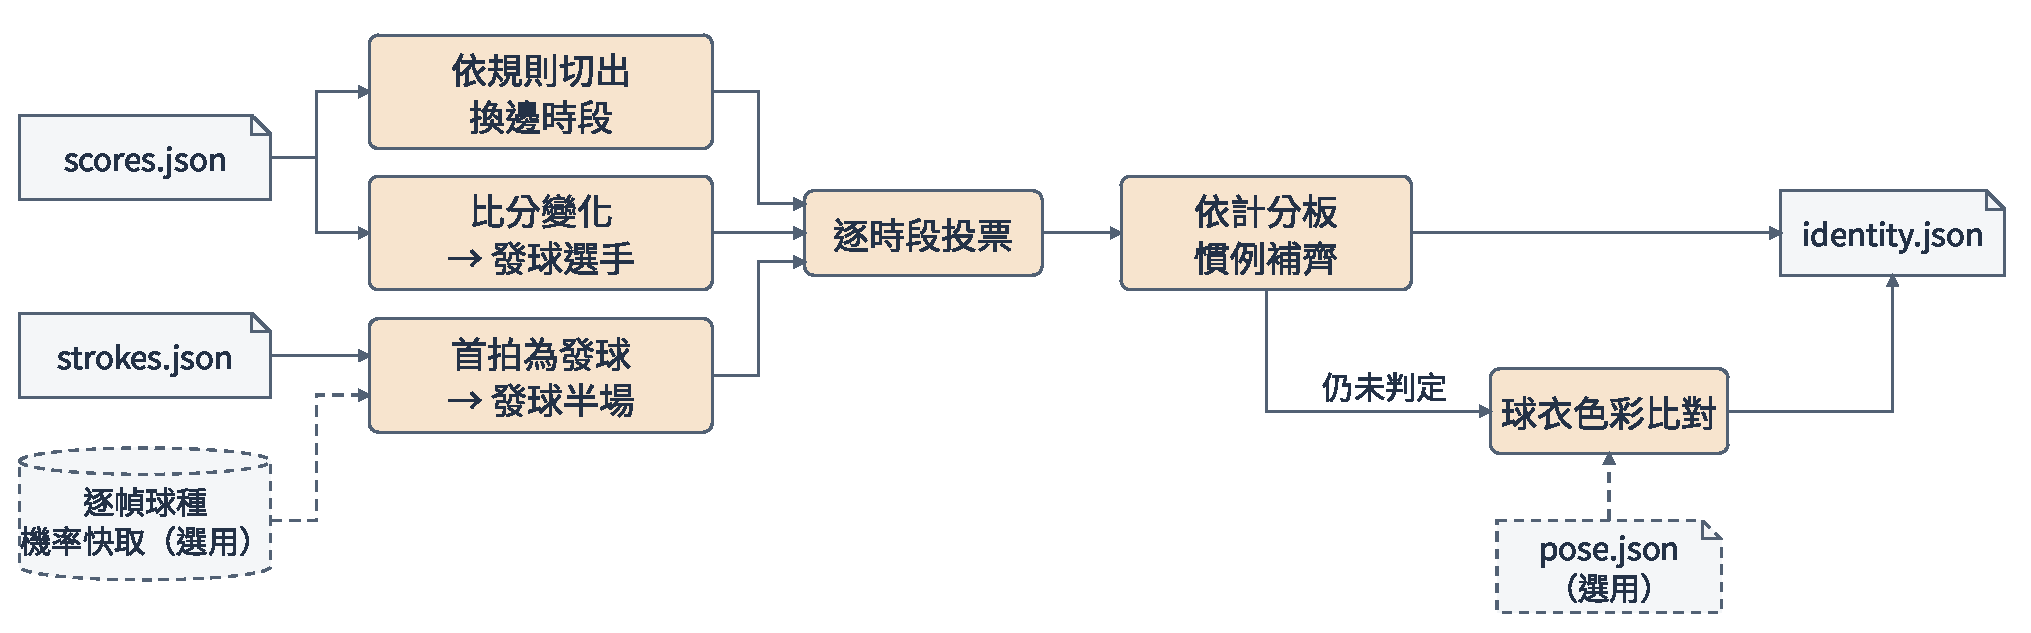
\includegraphics[scale=\flowscale]{identity-mapping.pdf}
  \caption{球員身分對應處理流程}
  \label{fig:identity-mapping-flow}
\end{figure}

\subsubsection{判定流程}

\textbf{誰發球。}落地得分制下，贏得回合的一方發下一球。\texttt{scores.json} 記錄的是回合開始前的比分，所以比較相鄰兩個片段，比分剛好加一分的選手就是下一個片段的發球者。

\textbf{發球者在哪一側。}回合第一拍的擊球者所在的半場，就是發球者的半場。但若擊球時刻偵測漏掉發球，第一拍其實是接發球，半場會整個判反。因此只採用 BST 判為發球的第一拍。其餘回合再從擊球時刻偵測的逐幀球種機率中找回發球，且只在發球類別與擊球者都明顯佔優時採用。

\textbf{投票與補齊。}同時知道發球選手與發球半場的回合各投一票，同一換邊時段內取多數。票數不足 5 票的時段，沿用最近已判定時段的結果，並依計分板慣例調整：列序固定的計分板每次換邊對調一次，隨場地換列的則不變。採用哪種慣例，由已判定時段之間是否對調推得。仍無法判定時，才比對兩側球員上衣與褲子的 HSV 色彩；連外觀也分不出來就留空，不做猜測。每個時段的判定依據（投票、慣例或外觀）都寫入 \texttt{identity.json}。

\section{使用者介面}
\label{sec:user-interface}

\subsection{概述}

\textbf{問題與目標：}前述各模組的輸出是十多份 JSON 檔，記錄每個回合的起訖、比分、球員骨架、羽球軌跡等。這些資料必須對照影片才看得懂，直接閱讀數字既無法判斷分析是否正確。本系統的使用者介面讓使用者不必操作指令列，就能完成「匯入影片、執行分析、對照影片回看結果」的完整流程，並把逐拍資訊疊回轉播畫面，讓分析結果可以被直接檢視。

\textbf{使用流程總覽：}如\figref{fig:ui-workflow}。

\begin{figure}[H]
  \centering
  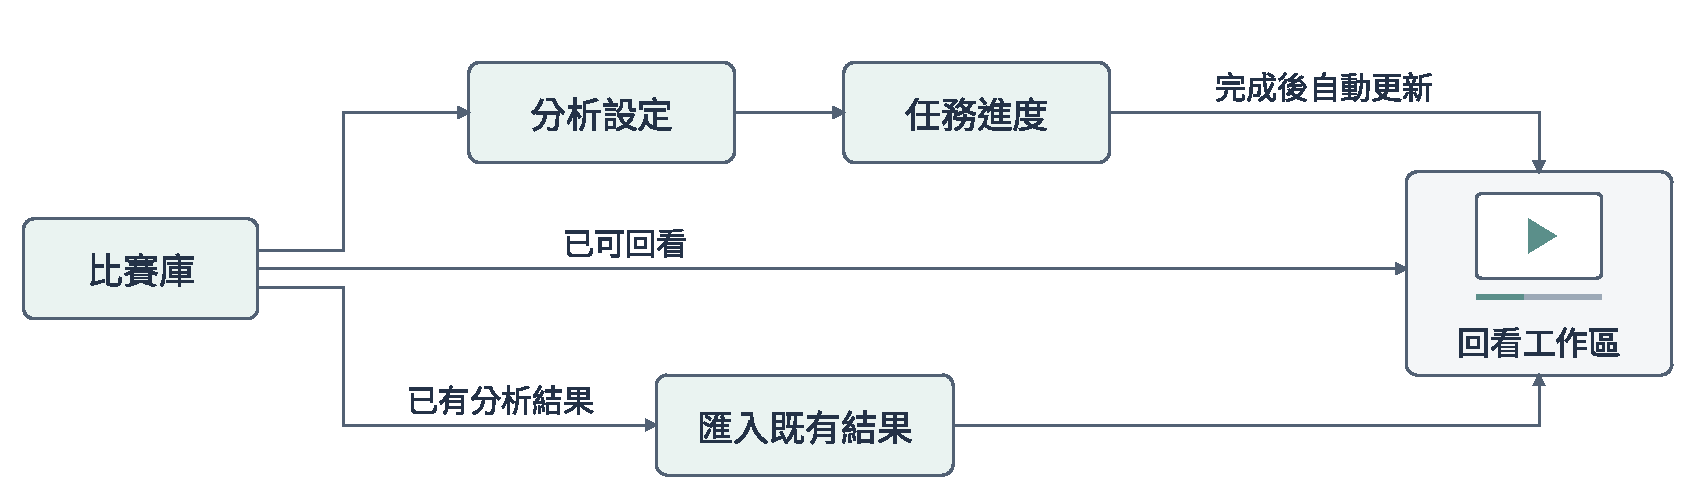
\includegraphics[scale=\flowscale]{ui-workflow.pdf}
  \caption{使用者介面操作流程}
  \label{fig:ui-workflow}
\end{figure}

比賽庫列出比賽資料夾中的每一場比賽及其分析狀態（\figref{fig:match-library}）。尚未分析的比賽從「分析設定」選擇要執行的項目（\figref{fig:analysis-settings}），分析在背景執行，完成後回看資料自動更新。已在其他環境完成分析的比賽，則可直接匯入既有結果，不需重新計算。

\begin{figure}[H]
  \centering
  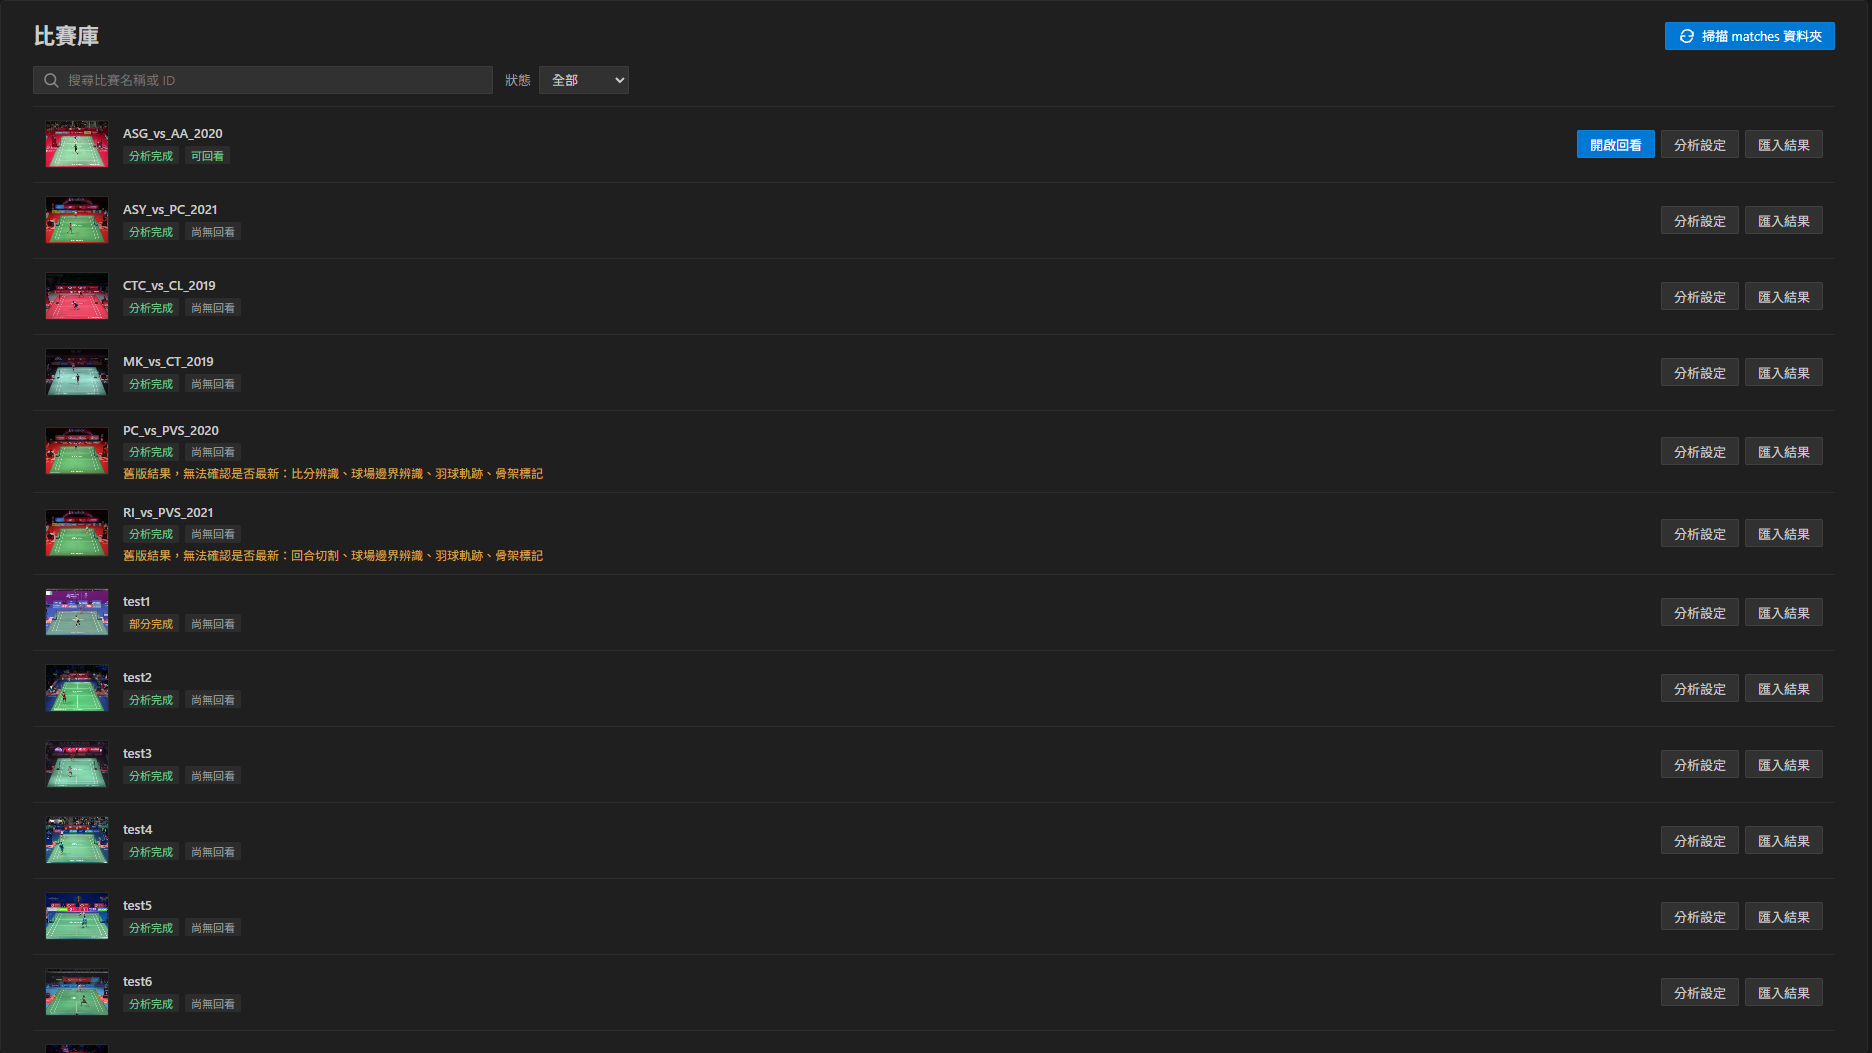
\includegraphics[width=\linewidth]{ui/match_library.png}
  \caption{比賽庫，每場比賽標示分析狀態與是否可回看}
  \label{fig:match-library}
\end{figure}

\begin{figure}[H]
  \centering
  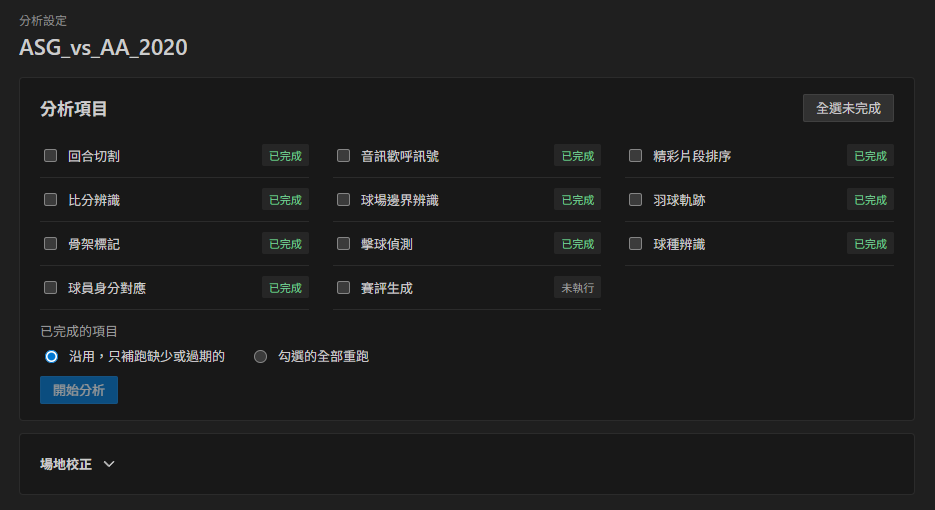
\includegraphics[width=0.850\linewidth]{ui/analysis_settings.png}
  \caption{分析設定，每個分析項目標示已完成、未執行或已過期}
  \label{fig:analysis-settings}
\end{figure}

\subsection{回看工作區}

回看工作區是介面的核心，由播放器、回合分析欄與時間軸三個區域組成（\figref{fig:review-workspace-full}）。三者共用同一個影片時間，任一區域的操作都會同步反映到另外兩區。

\begin{figure}[H]
  \centering
  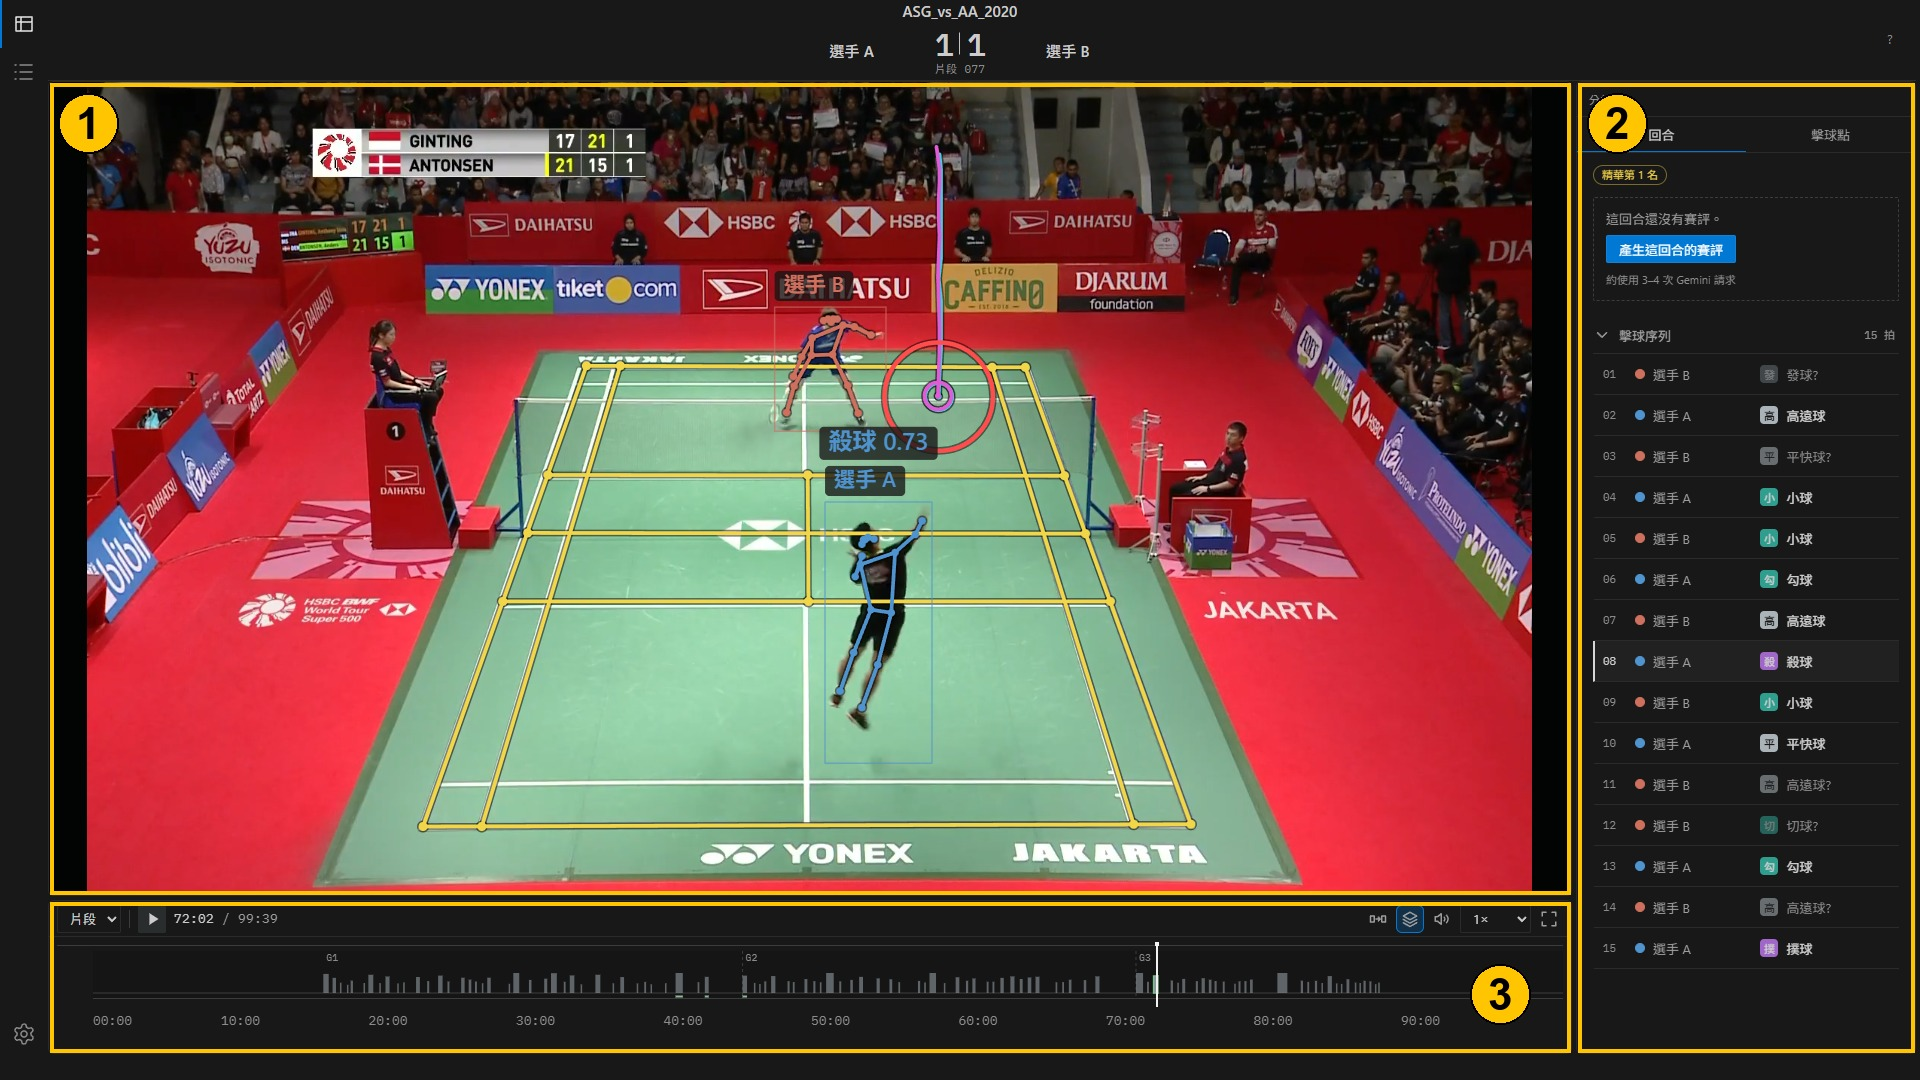
\includegraphics[width=\linewidth]{ui/review_workspace.jpg}
  \caption{回看工作區。\circnum{①} 播放器與疊圖 \circnum{②} 回合分析欄 \circnum{③} 時間軸}
  \label{fig:review-workspace-full}
\end{figure}

\subsubsection{播放器與疊圖}

播放器在轉播畫面上疊加各模組的分析結果，共 7 個圖層：球場線、骨架、選手標籤、羽球、球路拖尾、擊球閃圈與球種標籤（\figref{fig:overlay-layers}）。各圖層可以單獨開關，讓使用者直接用眼睛檢查各模組的結果，例如球場線是否貼合場地、骨架是否選對球員、軌跡是否跟著球走。

完整轉播中，回合只佔播出時間的約三成。「只播片段」模式會自動跳過回合之間的重播、休息與觀眾畫面，只播放分段模組切出的比賽片段。

\begin{figure}[H]
  \centering
  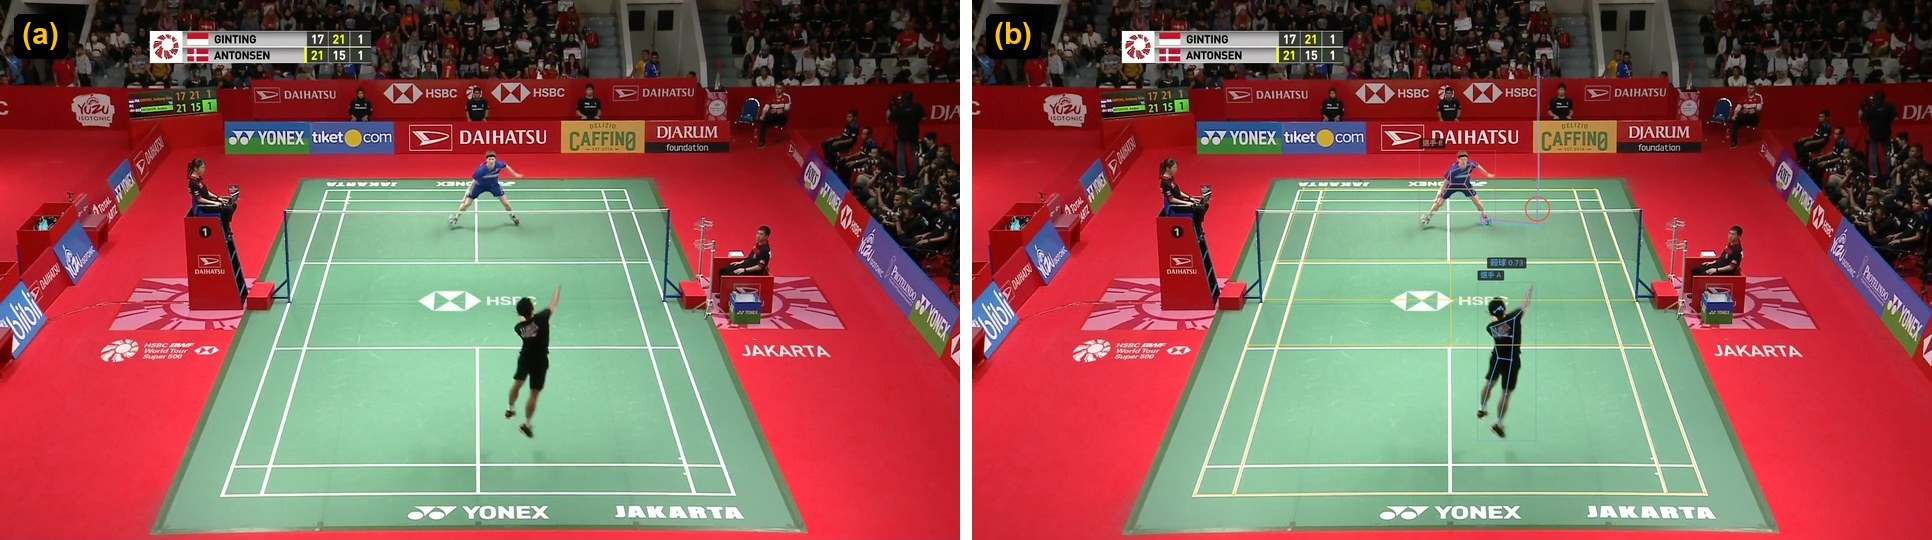
\includegraphics[width=\linewidth]{ui/overlay_layers.jpg}
  \caption{疊圖開啟前後。(a) 原始轉播畫面 (b) 開啟全部圖層}
  \label{fig:overlay-layers}
\end{figure}

\subsubsection{回合分析欄}

分析欄顯示目前回合的逐拍資訊，分為「回合」與「擊球點」兩個分頁（\figref{fig:inspector}）。

\begin{itemize}
  \item \textbf{擊球序列：}依序列出每一拍的擊球者與球種，信心度低於 0.5 的球種以淡色加問號標示。點選任一拍，影片即跳到該拍的擊球時刻。
  \item \textbf{精華標記：}精彩度排名在全場前 10\% 的回合，會在欄位頂端顯示排名徽章。
  \item \textbf{單回合賽評：}分析流程中的賽評階段只示範生成精彩排名前 3 的回合。其他回合由使用者在想看時按下「產生這回合的賽評」，每次約使用 3--4 次 Gemini 請求。產生後，回合摘要下方以「依據 \#1、\#2…」列出摘要所引用的擊球，點選即跳到該拍。逐拍賽評則附在擊球序列的每一拍下方，讓使用者能逐句對照影片確認賽評是否有所本。
  \item \textbf{擊球點：}以俯視球場標出本回合每一拍的擊球位置，依擊球順序連線，顏色區分兩名球員，可一眼看出回合中雙方的跑動與落點分布。
\end{itemize}

\begin{figure}[H]
  \centering
  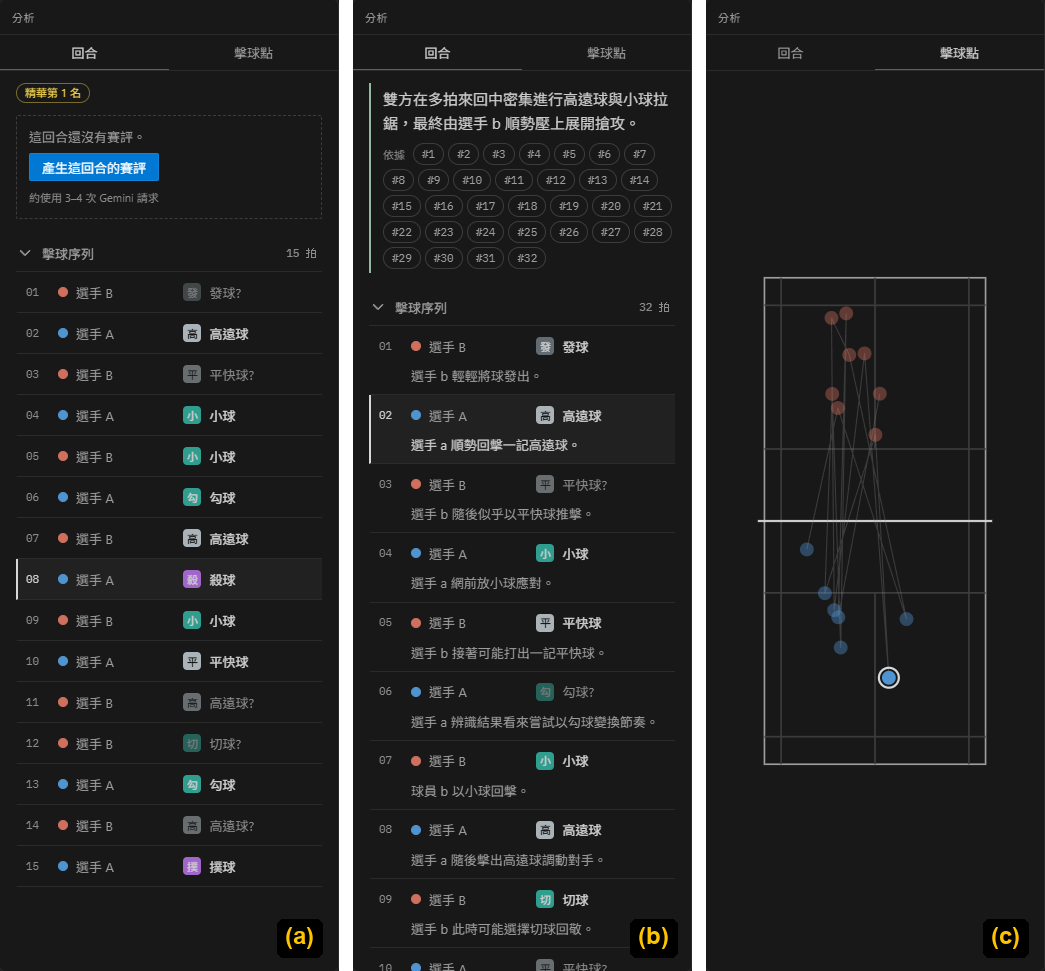
\includegraphics[width=0.950\linewidth]{ui/inspector.png}
  \caption{回合分析欄。(a) 擊球序列與精華排名 (b) 產生賽評後 (c) 擊球點分頁}
  \label{fig:inspector}
\end{figure}

\subsubsection{時間軸}

時間軸提供四種模式，各自呈現一種隨時間變化的分析結果（\figref{fig:timeline-modes}）。

\begin{itemize}
  \item \textbf{片段：}每個片段一根長條，高度為回合長度，並以 G1--G3 標示局數。
  \item \textbf{擊球：}依每片段的球種組成著色。
  \item \textbf{比分：}呈現雙方比分差距隨時間的變化，位於中線上方表示選手 A 領先、下方表示選手 B 領先。
  \item \textbf{歡呼：}顯示各片段的歡呼訊號，並以三角形與數字標示精彩度排名。
\end{itemize}

\begin{figure}[H]
  \centering
  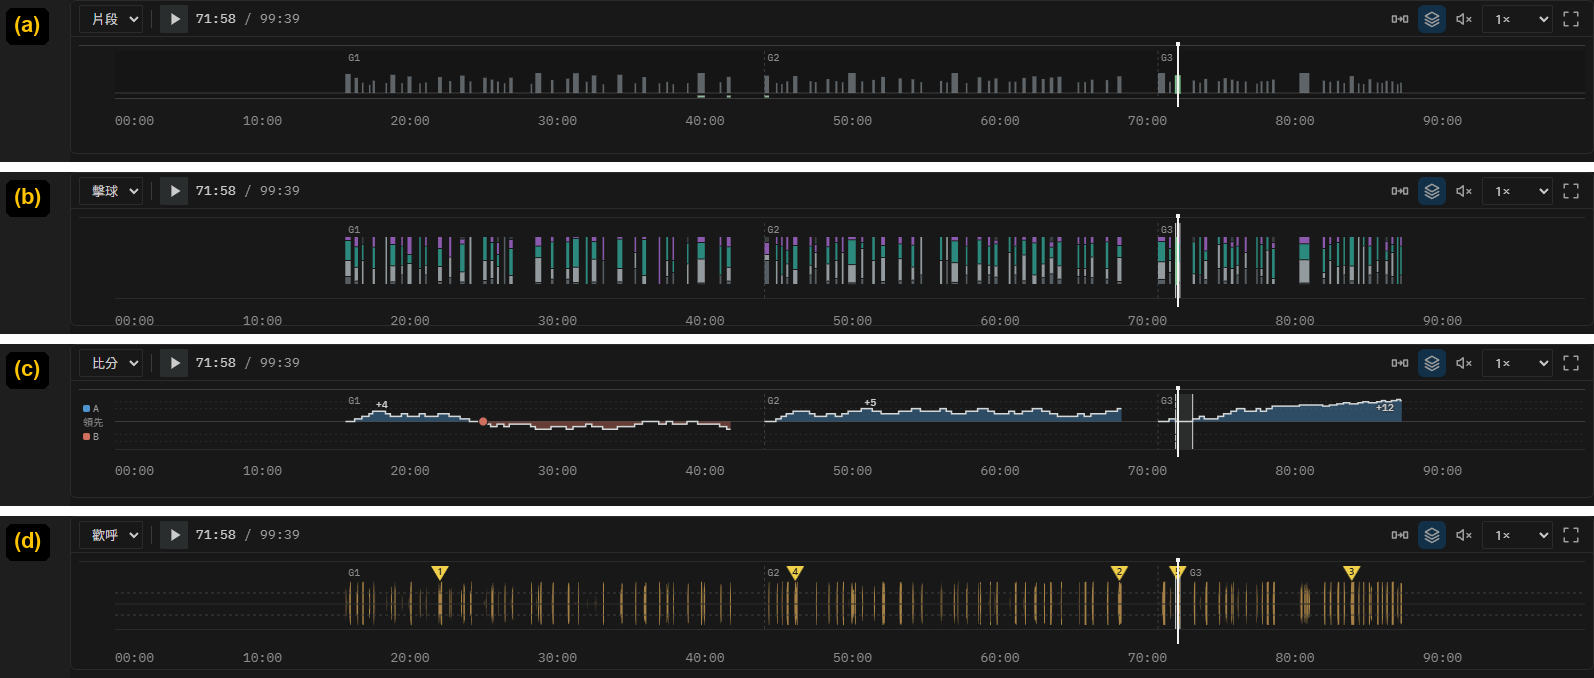
\includegraphics[width=\linewidth]{ui/timeline_modes.png}
  \caption{時間軸的四種模式（全場尺度）。(a) 片段 (b) 擊球 (c) 比分 (d) 歡呼}
  \label{fig:timeline-modes}
\end{figure}

時間軸可在「全場」與「單片段」兩種尺度間切換（\figref{fig:timeline-zoom}）。全場尺度用於掌握整場比賽的分布與走勢。雙擊任一片段即放大到該回合，此時每一拍成為一個點並標上球種縮寫，可以看出來回的節奏。

\begin{figure}[H]
  \centering
  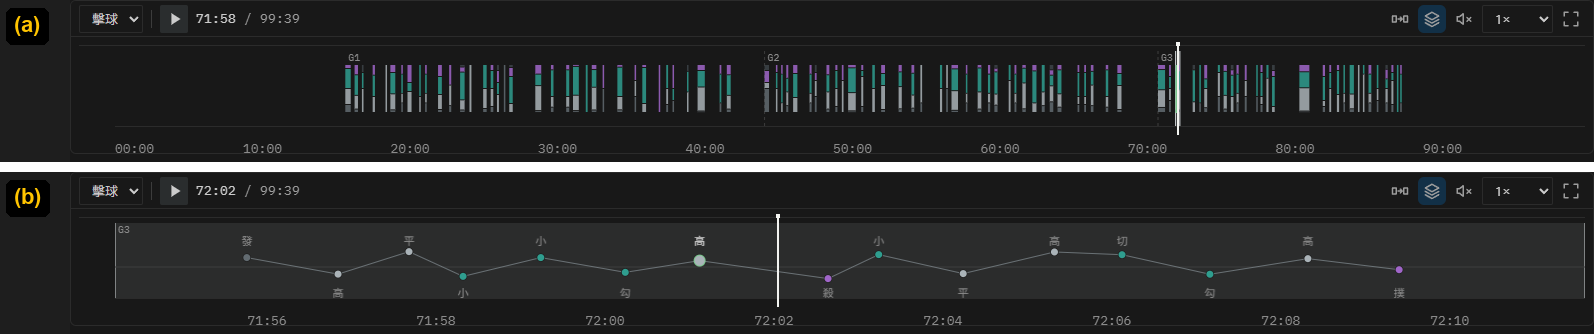
\includegraphics[width=\linewidth]{ui/timeline_zoom.png}
  \caption{擊球模式在兩種尺度下的呈現。(a) 全場 (b) 單回合}
  \label{fig:timeline-zoom}
\end{figure}

\subsection{分析任務與場地校正}

\textbf{分析計畫預覽：}使用者勾選分析項目時，介面即時列出執行計畫：哪些階段會執行、哪些沿用既有結果及其原因，以及計畫是否會呼叫 Gemini API（\figref{fig:plan-preview}）。若某些未勾選階段的上游結果會因這次分析而改變，介面也會列出這些將會過期的階段，回看時不會顯示過期的資料。

\begin{figure}[H]
  \centering
  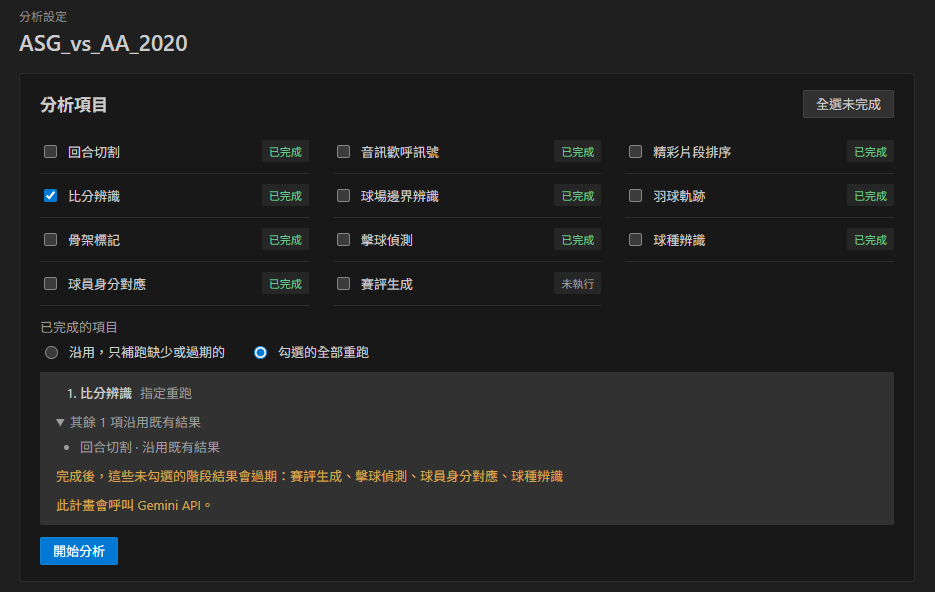
\includegraphics[width=0.850\linewidth]{ui/plan_preview.png}
  \caption{分析計畫預覽}
  \label{fig:plan-preview}
\end{figure}

\textbf{任務進度：}分析在獨立的背景程序中執行。任務頁顯示整體進度、各階段耗時與詳細記錄，使用者也可以隨時取消，取消時已完成的階段會保留，下次分析只需從中斷處繼續（\figref{fig:task-progress}）。

\begin{figure}[H]
  \centering
  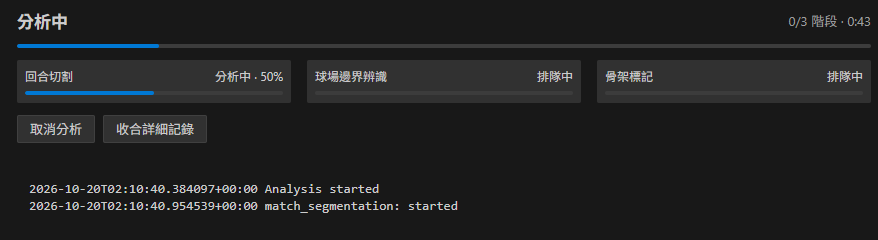
\includegraphics[width=0.798\linewidth]{ui/task_progress.png}
  \caption{任務進度，顯示整體與各階段的進度及詳細記錄}
  \label{fig:task-progress}
\end{figure}

\textbf{場地校正：}場地偵測是後續選人與站位換算的基礎，因此任務會先執行場地偵測，並把需要讀取球場的階段排到最後。球場一偵測完，介面即提示使用者檢查，分析設定頁自動展開場地預覽，其餘階段照常進行。若角點明顯偏移，使用者可直接在球場畫面上拖曳四個外角點，並以方向鍵逐像素微調（\figref{fig:court-calibration}）。保存後，尚未開始的階段直接使用新球場，已讀過舊球場的階段則自動重跑。

\begin{figure}[H]
  \centering
  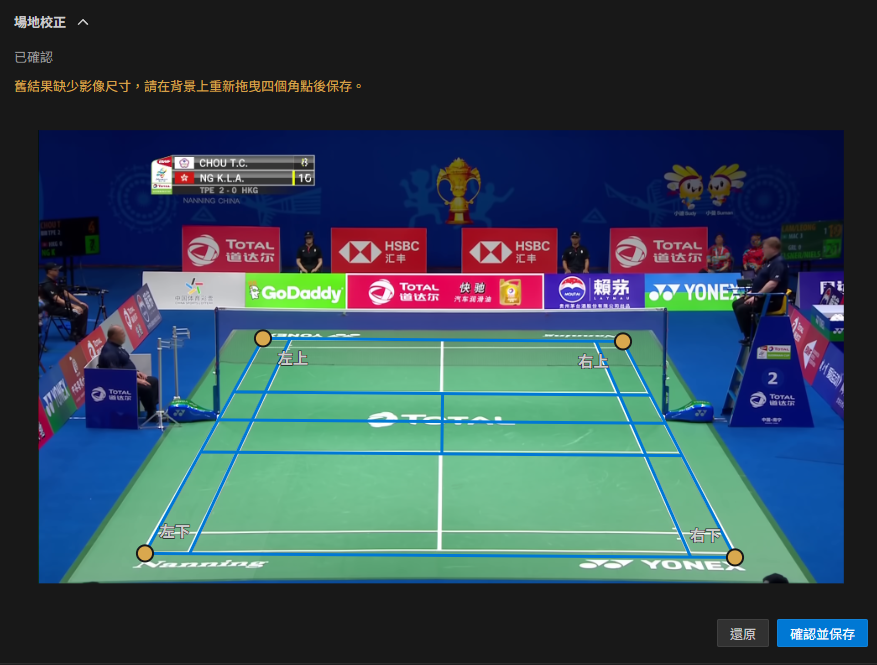
\includegraphics[width=0.797\linewidth]{ui/court_calibration.png}
  \caption{場地校正，拖曳四個外角點對齊球場邊線}
  \label{fig:court-calibration}
\end{figure}

\subsection{實作概要}

介面以 Vue 3 與 TypeScript 開發，並以 Electron 包裝為 Windows 桌面程式。分析本身仍由本機的 Python 服務執行，介面只負責送出分析任務與顯示進度。分析完成後，匯入程式會先驗證各階段的 JSON 是否完整、是否與影片相符，再整合成一份回看資料，介面只讀取這一份資料，不直接讀取各階段的原始輸出（\figref{fig:ui-architecture}）。骨架、軌跡等資料量較大的疊圖內容則按回合分開儲存，只在使用者打開疊圖時才讀取目前與下一個回合，避免開啟比賽時長時間等待。

\begin{figure}[H]
  \centering
  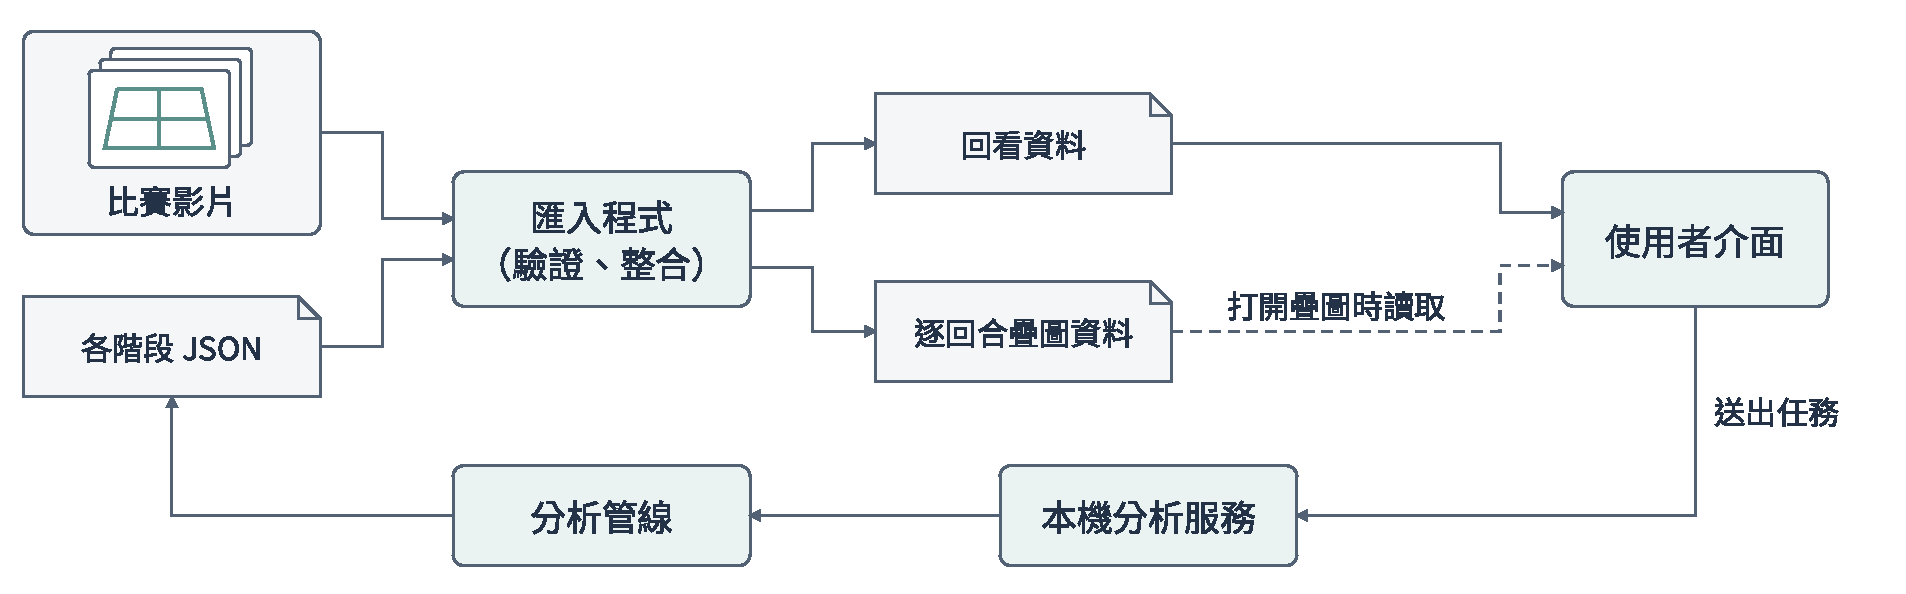
\includegraphics[scale=\flowscale]{ui-architecture.pdf}
  \caption{使用者介面實作架構}
  \label{fig:ui-architecture}
\end{figure}
